\documentclass[a4paper]{article}

\usepackage[english]{babel}
\usepackage[utf8x]{inputenc}
\hyphenation{mul-ti-lat-er-al}
\hyphenation{man-u-fac-tur-ing}

\usepackage[a4paper,top=2.5cm,bottom=2cm,left=3cm,right=3cm,marginparwidth=1.75cm]{geometry}

\usepackage{amsmath}
\usepackage{graphicx}
\usepackage[colorinlistoftodos]{todonotes}
\usepackage[colorlinks=true, allcolors=blue]{hyperref}
\usepackage{apacite}
\AtBeginDocument{\urlstyle{APACsame}}
\usepackage[section]{placeins}
\usepackage{adjustbox}
\usepackage{natbib}
\usepackage{booktabs}
\usepackage[bottom]{footmisc}  % Footnotes at bootom of page
\addto\captionsenglish{\renewcommand*\contentsname{Table of Contents}}

\title{\textbf{Patterns of Global and Regional Integration\\ in the East African Community}}
\author{Sebastian Krantz\footnote{Kiel Institute for the World Economy\\ \textit{Address:} Haus Welt-Club, Duesternbrooker Weg 148, D-24105 Kiel\\ \textit{E-mail:} sebastian.krantz@ifw-kiel.de\\\vspace{-10mm}}}
\date{July 20, 2024}

\begin{document}
\maketitle

\vspace{-5mm}
\begin{abstract} 
Using detailed global trade and novel Multi-Region Input-Output (MRIO) data, this paper examines the East African Community's (EAC) global and regional integration through trade, global, and regional value chains (GVCs and RVCs). With surgical attention to detail, the first part of the paper dissects key patterns and trends of EAC members' participation in global and regional trade and production networks at the aggregate, bilateral, sectoral, and bilateral-sectoral levels. The second part then provides causal reduced-form evidence for the economic benefits of EAC integration through trade, GVCs, and RVCs at the sector level. Findings imply that the region is moderately integrated into GVCs and RCVs but shows no overall trend towards greater integration. Regional integration is advancing in agriculture and food processing, and Kenya is becoming a more dominant regional supplier of manufactures. Integration through trade and GVCs positively affects economic development in the region, particularly deeper forward GVC linkages in manufacturing. Deepening regional trade and forward linkages yields additional economic benefits vis-a-vis global linkages. \\\\
\noindent \textbf{Keywords:} GVCs, RVCs, EAC, trade, regional integration, economic development\\
\textbf{JEL Classification:} F14; F15; O11
\end{abstract}



\section{Introduction}

Global Value Chains (GVCs), referring to the internationalization of production networks, have become a central topic in trade and development policy. With the entry into force of the African Continental Free Trade Area (AfCFTA) in May 2019 and some progress towards its full enactment, the potential of a large common market in Africa for increased GVC-related trade, both within Africa and between Africa and the world, is of great interest to economic researchers and policymakers. To gauge the potential implications and distributional side-effects of AfCFTA for trade and GVCs, it is instructive to study smaller efforts of regional integration and creation of common markets in Africa, as has been the case in East Africa with the East African Community (EAC). \newline 

(Re-)founded in 2000 by Uganda, Kenya, and Tanzania as a body to facilitate regional cooperation, the EAC quickly became a vehicle for economic integration. A customs union became operational in January 2005, with Kenya, the region's largest exporter, continuing to pay duties on some goods entering other countries on a declining scale until 2010 (EAC Customs Union Protocol, Article 11 and \citet{aloo2017free}). Rwanda and Burundi acceded in 2007, joining the customs union in 2009. The customs union expanded to a common market for goods, labor, and capital effective in 2010. In 2013, the Protocol for the Establishment of the EAC Monetary Union was signed, aiming for a monetary union within 10 years, subject to macro-fiscal convergence criteria. In 2016, the newly founded Republic of South Sudan joined the EAC, and the Democratic Republic of Congo joined in July 2022. Thus, the EAC, particularly the years following the customs union in 2005 and the common market in 2010, provides a small case study in light of AfCFTA's broader aims. \newline 

There is, by now, extensive academic and policy literature on the state, determinants, and consequences of integration into GVCs, including for countries at different income levels. As one of the first, \citet{Kummritz20162} examine patterns of GVC integration in low- and middle-income countries (LMICs) using the OECD TiVA database. They find that LMICs have become an integral part of GVCs and are driving their expansion, with a rising share in both the foreign content of global value added (VA) exports (9\% in 1995 to 24\% in 2011) and re-exported exports (9\% to 23\%). High-income economies use GVCs to outsource low-VA downstream production stages. However, over time, many developing economies move up the value chain. \newline 

The 2020 World Development Report (WDR), focusing on GVCs, classifies Africa as primarily a supplier of raw materials, with only a handful of countries (Morocco, Tunisia, Namibia, South Africa, Ethiopia, Kenya, and Tanzania) engaging in limited manufacturing \citep{world2020trading}. At the same time, GDP per capita grows most rapidly when countries enter limited manufacturing GVCs. The report estimates the average benefits from a 1 percent increase in GVC participation to boost per capita income by more than 1 percent, much more than the 0.2 percent income gain from standard trade. To enter GVCs, the report stipulates attracting FDI, improving access to finance, keeping labor costs low, trade liberalization, investments in ICT and transport infrastructure, and political stability. African economies score low in all of these dimensions. In particular, overvalued exchange rates and restrictive labor regulations raise the cost of labor: "Manufacturing labor costs in Bangladesh are in line with its per capita income, but in many African countries, labor costs are more than twice as high." \citep{world2020trading}. \newline

These policy conclusions are broadly echoed in much early and recent academic work. E.g., \citet{fernandes2022determinants}, using a panel with more than 100 countries and a novel identification strategy, show that factor endowments, geography, political stability, liberal trade policies, FDI inflows, and domestic industrial capacity are key determinants of GVC participation, whereas traditional exports are less important. The findings are commensurate with \citet{antras2020geography}, which develop a general-equilibrium framework where trade costs imply a concentration of downstream production stages in central locations/countries (close to final demand). \citet{kowalski2015participation} also find that proximity to manufacturing hubs in Europe, North America, and East Asia, domestic market size, and the level of development, are key determinants of GVC participation. \newline
  
 \citet{foster2015global} provide one of the first comprehensive analyses of GVCs in Africa, using the EORA 25 sector database over 2000-2011. They find that Africa is more involved in GVCs than many other developing regions but mainly supplies primary goods. Downstream involvement is relatively small and shows little improvement in 1995-2011. GVC involvement is also very heterogeneous across African countries, with some relatively successful countries (Tunisia, South Africa) heavily involved in (downstream) GVCs. Inner-African GVCs are also small in most African countries, with several exceptions in southern Africa. The EU is Africa's biggest GVC partner, with increasing shares of (South-)East Asia and other transition countries. \newline

\citet{kowalski2015participation} study GVC participation in Africa, the Middle East, and Asia, showing that developing countries reap important benefits from GVC participation through both forward and backward linkages, including enhanced productivity, export diversification, and sophistication. Analyzing export competitiveness, they find that Asia dominates more advanced products such as electronic equipment or motor vehicles. In contrast, African and Middle Eastern regions are competitive in agriculture, food processing, and less advanced manufacturing. While all regions have become more competitive, they find no trend towards GVC-led industrialization in Africa. \newline 

\citet{balie2019does} present a careful analysis of bilateral-sectoral GVC linkages in SSA with an emphasis on food processing GVCs and show that SSA's participation in these chains is substantial. This is driven by a handful of countries, including Kenya and Uganda, where the share of agriculture in total GVC participation is 30\%, and in Kenya, the food processing sector is at 15\%. They further show that bilateral trade policy is a key determinant in shaping SSA's GVC integration in the food sector, with high tariffs detrimental to GVC participation. They also echo \citet{foster2015global} that SSA GVC participation is high - at 40\%, comparable to China and India. Africa is also the continent with the highest forward integration - around 25\% of domestic VA (DVA) produced in SSA are inputs for other countries' exports and over 35\% in North Africa. \newline

There has also been some GVC and RVC-related work on African regional economic communities (RECs). Notably, \citet{obasaju2021regional} examine the impact of regional integration on upgrading through GVCs (proxied by DVA in exports per capita) in the EAC, Southern African Customs Union (SACU) and Economic Community of West African States (ECOWAS) in 2000-2015. They show that regional integration and FDI are not significant drivers of upgrading but lagged backward GVC participation is. They also find weak positive effects of regional integration on labor productivity in the EAC and SACU (the communities with stronger trade integration). Regional hegemons (Kenya, South Africa, and Nigeria) have weak backward linkages with other members. \newline 

\citet{tinta2017determinants} studies determinants of GVC participation in ECOWAS and finds that intra-regional trade is not a significant predictor of trade openness, but backward GVC participation is. Further, trade diversification is a key predictor of backward GVC participation. \citet{engel2016sacu} provide a detailed analysis of GVC integration, position, and performance of SACU members (Botwana, Lesotho, Namibia, South Africa and Eswatini). They show that the SACU region is moderately integrated into GVCs in relatively upstream tasks, but the scale and nature of integration vary by country, with South Africa and Namibia being the most integrated. South Africa remains a moderately important player in global trade networks and an important regional hub. Lesotho shows a rapid increase in GVC integration, Namibia a moderate increase, whereas Botswana and Eswatini appear stagnant or in decline. Overall growth in GVC participation in services is stronger than in manufacturing. South Africa is the only country with strong forward GVC integration and a major source of foreign content for the other members, which are more integrated into RVCs than GVCs. China has grown significantly as a source of foreign content, but the EU remains the predominant partner for forward GVC participation. \newline 

\citet{lwesya2022integration} studies GVC integration in the EAC with respect to economic upgrading using UNCTAD-Eora data from 2005 to 2018. This analysis is largely complementary to the one carried out in this paper. He computes measures of backward and forward integration and finds that Kenya, Tanzania, and Uganda are relatively better integrated into GVCs, with Kenya having the deepest level of integration, especially in terms of indirect VA and forward integration. Overall, the EAC's participation in GVCs is in upstream low- and middle-VA production activities. Using a cross-country panel regression framework predicting DVA in exports, which includes GVC indicators and other macroeconomic indicators, he finds that domestic credit, foreign direct investment, the quality of institutions, and foreign VA (FVA) have significant positive effects, but observes no such effects for measures of human capital, infrastructure quality, and GDP per capita. The analysis is focused on economic upgrading and does not provide a detailed bilateral and sector-level exposition of the region's integration into GVCs and RVCs. He also does not provide a detailed examination of how different forms of trade and GVC participation affect economic growth, and does not establish economic causality between any of the studied factors and DVA in exports. \newline

This paper adds to our understanding of GVCs and regional integration in the EAC in the following significant respects: (1) it uses better data, including gross trade flows data and the EMERGING MRIO tables, which include IO/SUT/SAM tables for 4 EAC countries; (2) it conducts a detailed examination of EAC members global and regional integration using both gross trade flows and VA content shares, paying close attention to specific bilateral linkages and sector-level patterns; (3) it constructs metrics to track regional integration in VA terms and uses them to measure progress in recent years; (4) It examines the positioning of EAC members and sectors in GVCs and (5) revealed comparative advantage in gross and VA terms; (6) It analyzes the effect of conventional trade, GVC, and RCV integration on GDP using a bilateral-sector-level regression framework with triple fixed effects and instrumental variables for GVC participation following \citet{Kummritz20161}. Thus, it presents a rigorous and detailed study of the region's global and regional integration through trade and value chains using the best currently available data and attempts to establish economic causality between different forms of trade and economic growth. 


\section{Data}

Most GVC analysis uses Inter-Country Input-Output tables (ICIOs), such as those published by the OECD (TiVA) or the World Input-Output Database (WIOD)  \citep{timmer2012world}. These, however, focus on OECD countries, with very limited coverage of SSA. This paper, therefore, uses two Multi-Region Input-Output (MRIO) databases that are global in scope. \newline 
 
The first is the EORA 26 Global MRIO \citep{lenzen2012mapping, lenzen2013building}, which has extensive coverage of 189 countries and 26 sectors from 1990-2015 and uses 74 country IOT/SUTs and detailed international macroeconomic and trade data as input. EORA relies on sophisticated methods to impute, harmonize, and interpolate data across countries and time and is thus less accurate than the OECD or WIOD tables. Particularly for small countries like EAC members, data can be highly distorted. The Kenya 2010 IOT is the only source of EAC national data used in EORA \citep{lenzen2013building}. A 2021 EORA update added administrative data through 2018 and WEO-based forecasts through 2021. It introduced a large structural break in the time series in 2016, with different macroeconomic totals and GVC indicators for EAC members. The analysis thus emphasizes the initial release through 2015. Since the EAC customs union only became operational in 2005, I consider EORA 26 tables from 2000 onwards. Data from 1990 shows no interesting trends in GVC engagement. EORA is denominated in thousands of current USD at basic prices\footnote{The basic price is the amount receivable by the producer from the purchaser for a unit of a good or service produced, as output minus any tax payable, and plus any subsidy receivable. It excludes any transport charges invoiced separately by the producer.}. Appendix Figure \ref{fig:EORADQMT} shows the official EORA data quality reports for 6 EAC countries\footnote{While global GDP is broadly consistent with representative estimates, the GDP of EAC countries is highly distorted. Most notably, Tanzania's GDP is decreasing in the data. The situation is better for exports, whose level and sectoral composition are roughly consistent with estimates from other sources. Thus, detailed analysis and results from EORA should be treated with great caution, particularly for Tanzania.}. Despite its shortcomings, EORA has enabled significant research on GVCs in Africa. \newline 

Due to the shortcomings of EORA in terms of accuracy and usage of national data for developing countries, I also employ the more recently introduced EMERGING (EM) MRIO tables \citep{huo2022full}. This impressive effort has created a global MRIO database covering 245 countries and territories in 135 sectors for the years 2015-2019. A recent update (v2) also provides a table for 2010. EM uses 111 national IO/SUT/SAM tables alongside detailed trade and macroeconomic data. In particular, the UN Comtrade database is utilized to the fullest extent to provide greater sectoral detail than EORA. Macroeconomic data from national statistical offices is used where available and reconciled (scaled) using World Bank data. The purpose of the MRIO is to provide greater detail and accuracy for emerging economies than EORA. From EAC countries, EM uses a SAM and sectoral GDP from Uganda up to 2016 and the same information up to 2019 for Rwanda and Kenya. For Tanzania, EM uses a SAM and an IO table up to 2017. For Burundi, Congo (DR), and South Sudan, only international data is available. Thus, EM incorporates, to the greatest extent possible, national data from these EAC countries in a harmonized global MRIO framework. EM is denominated in millions of current USD at basic prices. \newline

The WDR also provides GVC indicators using EORA 2015, and \citet{mancini2023positioning} provide corresponding GVC positioning indicators following \citet{fally2012production}, \citet{antras2012measuring} and \citet{antras2013organizing, antras2018measurement}. These pre-computed indicators are used to verify manually computed indicators. This is important because I aggregate the non-EAC World and/or sectoral resolution for different indicators to lift computational constraints\footnote{EMERGING has 245 countries/territories and 134 sectors, implying 32,830 rows and columns or 1 billion records in the transaction matrix. It is computationally infeasible for me to compute GVC indicators directly on these tables, and also the full EORA database (186 x 26 = 4836 rows and columns observed over 21 years) strains my computing resources for non-trivial GVC indicators. \vspace{-7mm}} and enable comparisons across databases. In particular, for backward GVC indicators the non-EAC World is aggregated into 11 geographic and trade regions summarised in Table \ref{tab:ctry}, and, in more detail, in Appendix Table \ref{tab:ctrydet}. 


\begin{table}[h!] \vspace{-2mm}
\centering
\caption{\label{tab:ctry}\textsc{Regional Aggregation}}
\vspace{2mm}
\begin{tabular}{llrr} \toprule
& & \multicolumn{2}{c}{\textit{Countries \& Territories}} \\
\textit{Region} & \textit{Description} & EORA & EMERGING \\ \midrule
EAC & East African Community & 7 & 7 \\
SSA & Sub-Saharan Africa (Excluding EAC) & 38 & 41 \\
EUU & European Union + UK & 28 & 29 \\
ECA & Europe and Central Asia (Non-EU) & 26 & 29 \\
MEA & Middle East and North Africa & 20 & 21\\
NAC & North America and Canada & 3 & 13 \\
LAC & Latin America and Carribean & 32 & 44 \\
ASE & ASEAN & 10 & 10 \\
SAS & South Asia & 8 & 9 \\
CHN & China & 3 & 3 \\
ROA & Rest of Asia & 7 & 14 \\
OCE & Oceania & 6 & 22 \\ \midrule
SUM: & 7 EAC Members + 11 World Regions & 188 & 245
 \\ \bottomrule
\end{tabular}
\vspace{-5mm}
\end{table}
\FloatBarrier


To verify EM, \citep{huo2022full} develop a broad sector classification of 17 sectors and mappings it to major global ICIOs (EXIOBASE3rx, OECD-TiVA, EORA, GTAP, and EM). I use these mappings to report results at the sector level. Most GVC indicators are computed at the full sector resolution using STATA's ICIO package \citep{belotti2020icio} and the default source-based exporter perspective \citep{borin2019measuring} also used in the WDR, which permits aggregation of GVC indicators across sectors. Table \ref{tab:sec} shows the 26 EORA sectors\footnote{3-character sector codes are assigned and used throughout the paper based on the authors discretion, but not provided in the raw data. These codes are purely descriptive and do not correspond to any formal classification.} and their mapping to broad sectors. Appendix Table \ref{tab:EMSec} shows the mapping for EM. 
 
 
\begin{table}[h!]
\centering
\caption{\textsc{EORA 26 Sectors and Mapping to Broad Sectors}}
\label{tab:sec}
\vspace{2mm}
\resizebox{\textwidth}{!}{
\begin{tabular}{llll}
  \toprule
Code & EORA 26 Sector Definition & Code & Broad Sector Definition of \citet{huo2022full} \\ 
  \midrule
AGR & Agriculture & AFF & Agriculture, Hunting, Forestry \& Fishing \\ 
  FIS & Fishing & AFF & Agriculture, Hunting, Forestry \& Fishing \\ 
  MIN & Mining and Quarrying & MIN & Mining \& Quarrying \\ 
  FBE & Foods \& Beverages & FBE & Food Production, Beverages \& Tobacco \\ 
  TEX & Textiles and Wearing Apparel & TEX & Textiles, Leather \& Wearing Apparel \\ 
  WAP & Wood and Paper & WAP & Wood, Paper \& Publishing \\ 
  PCM & Petroleum, Chemical and Non-Metallic Mineral Products & PCM & Petroleum, Chemicals \& Non-Metallic Mineral Products \\ 
  MPR & Metal Products & MPR & Metal \& Metal Products \\ 
  ELM & Electrical and Machinery & ELM & Electrical \& Machinery \\ 
  TEQ & Transport Equipment & TEQ & Transport Equipment \\ 
  MAN & Other Manufacturing & MAN & Manufacturing \& Recycling \\ 
  REC & Recycling & MAN & Manufacturing \& Recycling \\ 
  EGW & Electricity, Gas and Water & EGW & Electricity, Gas \& Water \\ 
  CON & Construction & CON & Construction \\ 
  MRE & Maintenance and Repair & SMH & Sale, Maintenance \& Repair of Vehicles; Fuel; Trade; Hotels \& Restaurants \\ 
  WTR & Wholesale Trade & SMH & Sale, Maintenance \& Repair of Vehicles; Fuel; Trade; Hotels \& Restaurants \\ 
  RTR & Retail Trade & SMH & Sale, Maintenance \& Repair of Vehicles; Fuel; Trade; Hotels \& Restaurants \\ 
  AFS & Hotels and Restraurants & SMH & Sale, Maintenance \& Repair of Vehicles; Fuel; Trade; Hotels \& Restaurants \\ 
  TRA & Transport & TRA & Transport \\ 
  PTE & Post and Telecommunications & PTE & Post \& Telecommunications \\ 
  FIB & Finacial Intermediation and Business Activities & FIB & Financial Intermediation \& Business Activity \\ 
  PAD & Public Administration & PAO & Public Administration; Education; Health; Recreation; Other Services \\ 
  EHO & Education, Health and Other Services & PAO & Public Administration; Education; Health; Recreation; Other Services \\ 
  PHH & Private Households & PAO & Public Administration; Education; Health; Recreation; Other Services \\ 
  OTH & Others & PAO & Public Administration; Education; Health; Recreation; Other Services \\ 
  REI & Re-Export \& Re-Import & PAO & Public Administration; Education; Health; Recreation; Other Services \\ 
   \bottomrule
\end{tabular}
}
\end{table}
\FloatBarrier

To complement and verify MRIO table results, I also use gross trade flow data from CEPII's BACI \citep{CEPIIBACI} (HS 1996 version) and the IMF's Direction of Trade Statistics (DOTS) \citep{IMFDOTS}. EM's goods-producing sectors are identical to the 2-digit HS codes so that BACI can be aggregated to match the MRIO databases using the mapping in Table \ref{tab:EMSec}. The DOTS database only records aggregate bilateral trade, with imports denominated in Cost Insurance Freight (CIF) terms (including transport and insurance costs).  


\section{Trade}

In light of the known macroeconomic inconsistencies in EORA for EAC countries and that VA flows are estimated from gross flows, I begin by examining EAC integration through trade using BACI, DOTS, and gross total and intermediate flows from the EORA and EM MRIO tables. 

\subsection{Gross Trade Flows}

Figure \ref{fig:MIG} shows diagrams of EAC trade flows averaged over 2010-2019. All databases emphasize Kenya as regional trading hegemon, followed by Uganda and Tanzania, but EORA gives disproportional weight to Kenya and shrinks the other countries, whereas EM overemphasizes Rwanda and Uganda a bit and also shrinks Congo. Notably, the large exports from Congo to Tanzania are not reflected in either EORA or EM. An examination of BACI reveals that 88\% of this 550 million USD flow is copper and 7.4\% precious metals. Congo does not trade with other EAC members to a similar extent. \newline

 The bottom half of Figure \ref{fig:MIG} includes the rest of the world (ROW) as a trading partner. In all databases, trade with ROW dwarfs inner-EAC trade. According to BACI, inner EAC trade is 15 times smaller than EAC trade with ROW, in DOTS 14.9 times, in EORA 17.5 times, and in EM it is 22.9 times smaller. When excluding South Sudan and Congo, the ratios increase to 18.6 (BACI), 19.5 (DOTS), 14.9 (EORA (decrease)), and 19.7 (EM). \newline

\begin{figure}[h!] 
\centering
\centering
\caption{\label{fig:MIG}\textsc{Average Gross Trade Flows from 2010-2019: 4 Databases: USD Billions}}
\vspace{2mm}
\resizebox{\textwidth}{!}{
\begin{tabular}{cccc}
CEPII BACI & IMF DOTS & EORA (Basic Prices) & EMERGING (Basic Prices) \\
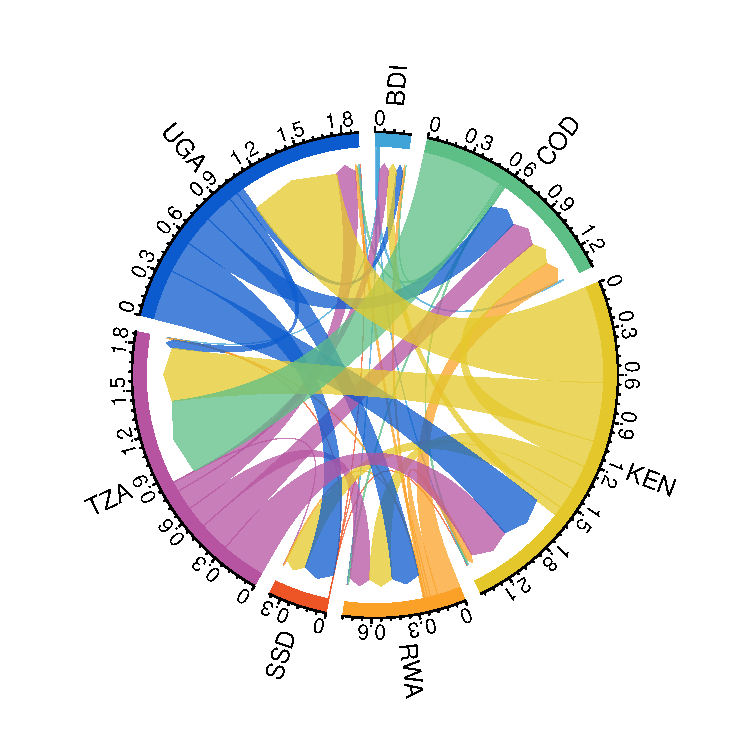
\includegraphics[width=0.4\textwidth, trim= {1.3cm 0.8cm 1.1cm 1cm}, clip]{"../Figures/REV/BACI_MIG_2010_19.pdf"} & 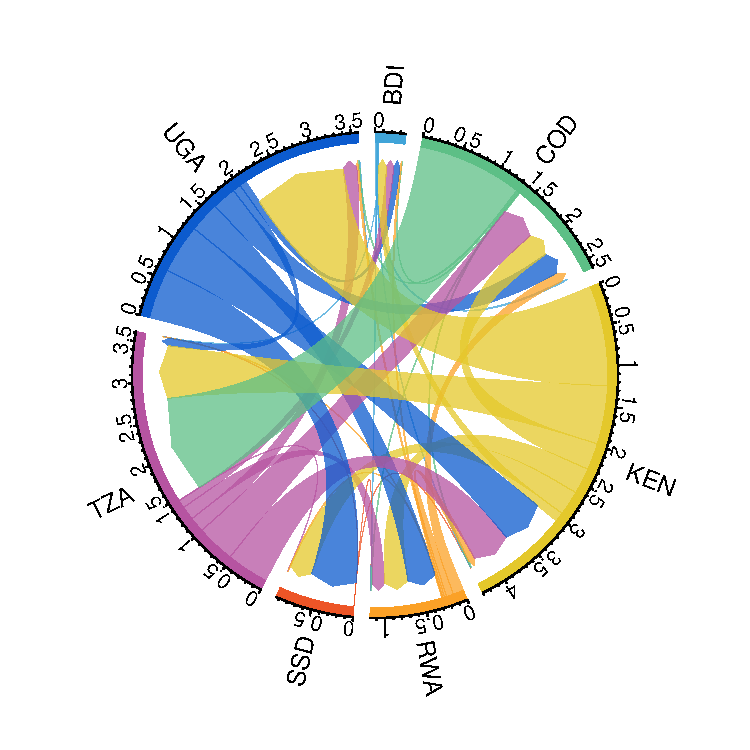
\includegraphics[width=0.4\textwidth, trim= {1.3cm 0.8cm 1.1cm 1cm}, clip]{"../Figures/REV/DOT_MIG_2010_19.pdf"} &
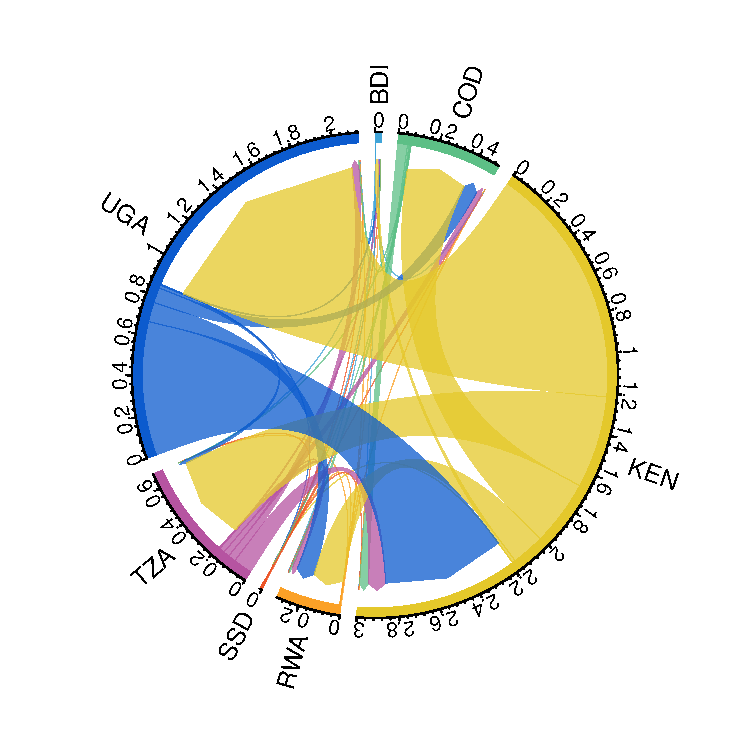
\includegraphics[width=0.4\textwidth, trim= {1.3cm 0.8cm 1.1cm 1cm}, clip]{"../Figures/REV/EORA_MIG_2010_19.pdf"} & 
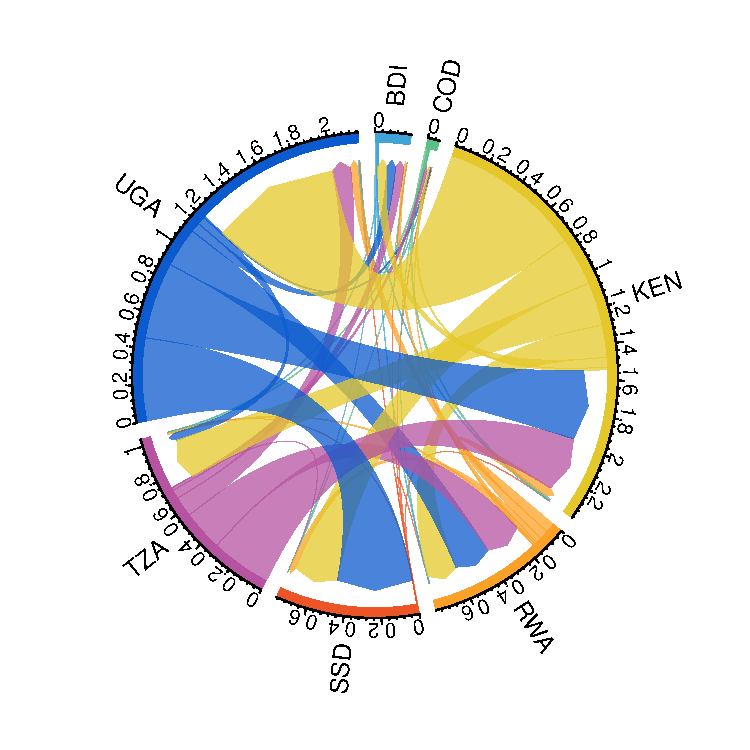
\includegraphics[width=0.4\textwidth, trim= {1.3cm 0.8cm 1.1cm 1cm}, clip]{"../Figures/REV/EM_MIG_2010_19.pdf"} \\
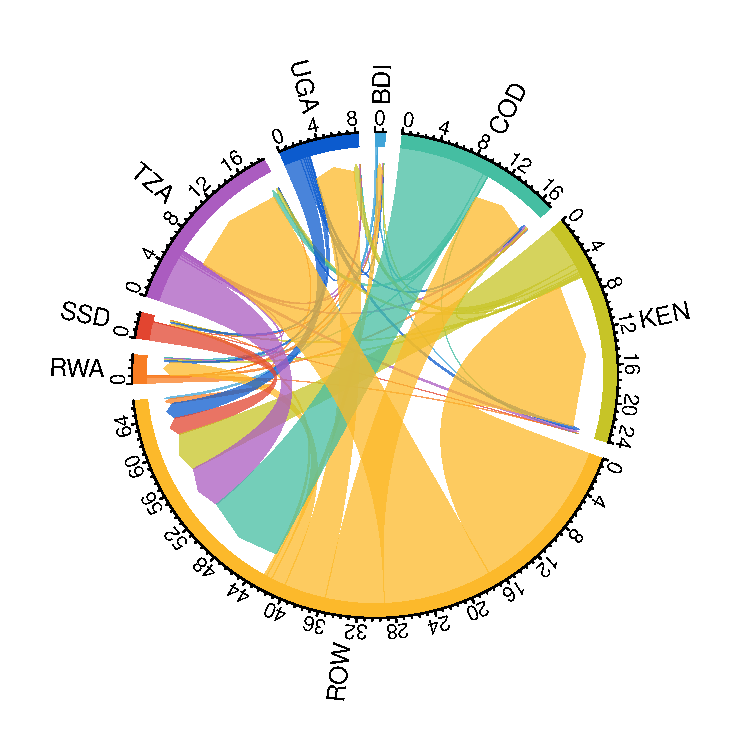
\includegraphics[width=0.4\textwidth, trim= {0.85cm 0.8cm 1cm 1cm}, clip]{"../Figures/REV/BACI_MIG_2010_19_ROW.pdf"} & 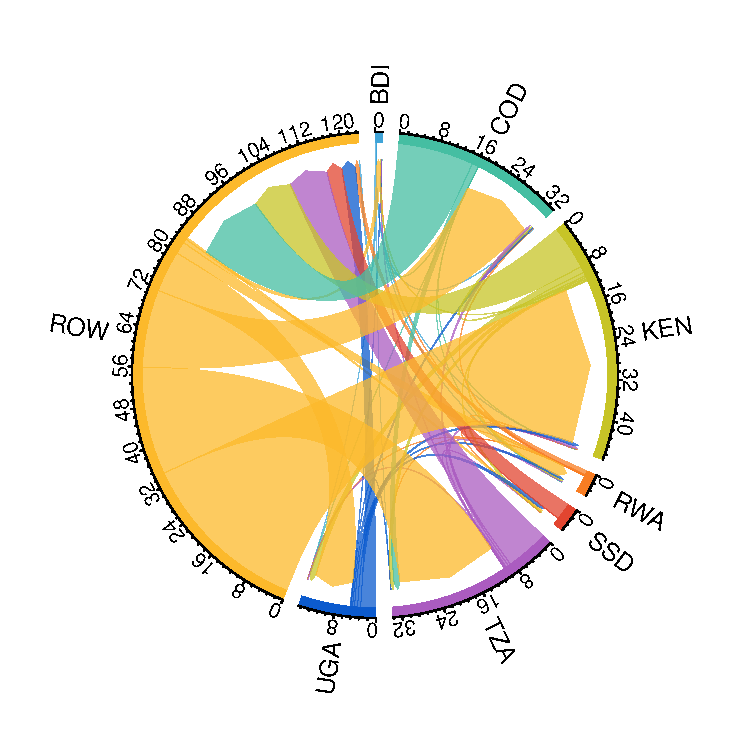
\includegraphics[width=0.4\textwidth, trim= {0.8cm 0.8cm 1cm 1cm}, clip]{"../Figures/REV/DOT_MIG_2010_19_ROW.pdf"} &
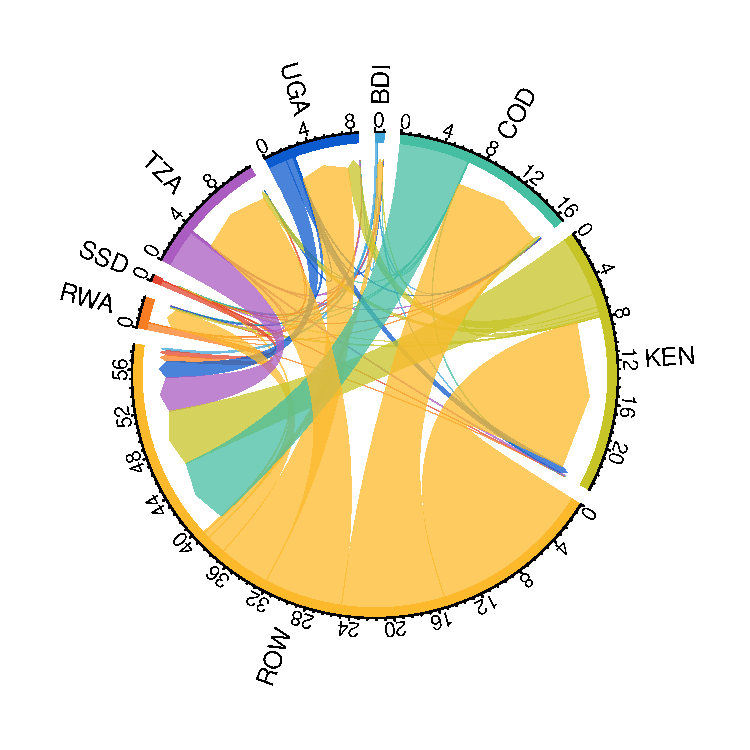
\includegraphics[width=0.4\textwidth, trim= {1cm 0.8cm 0.9cm 1cm}, clip]{"../Figures/REV/EORA_MIG_2010_19_ROW.pdf"} &
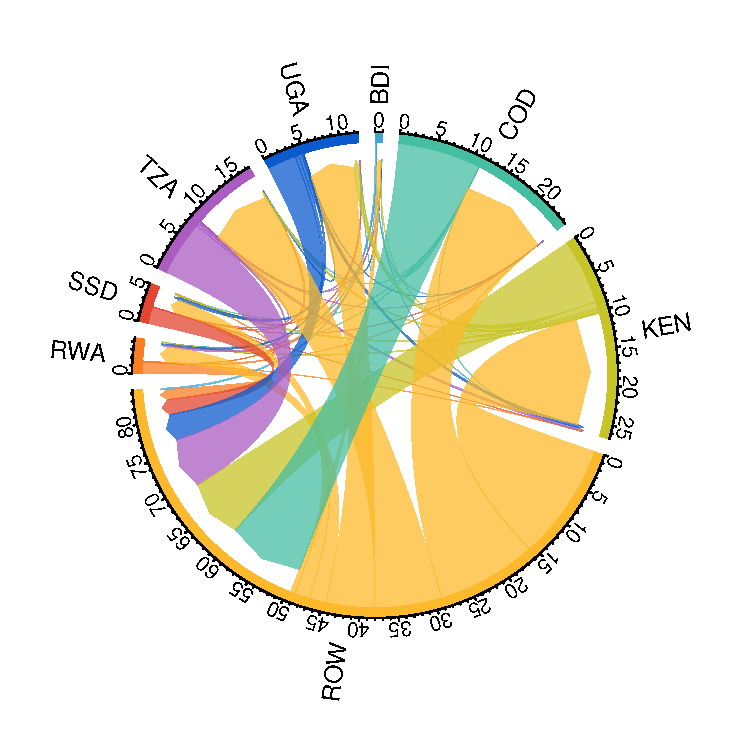
\includegraphics[width=0.4\textwidth, trim= {0.8cm 0.8cm 1cm 1cm}, clip]{"../Figures/REV/EM_MIG_2010_19_ROW.pdf"}
\end{tabular}
}
\raggedright
\scriptsize 
\emph{Notes:} Figure shows the mean of bilateral gross trade flows over years 2010-19 recorded in billions of current USD. The top panel shows inner-EAC flows; the bottom panel includes ROW as a trading partner. The circular axis records the total flows (exports + imports) for each partner. Produced using the \emph{migest} R package \citep{rmigest}.
\end{figure}
\FloatBarrier

Figure \ref{fig:EAC_ROW_Ratios} shows the evolution of this ratio for the five early EAC members (EAC5), smoothed using a backward-looking 5-year moving average (MA). Up to 2017, trade with ROW has grown faster than inner-EAC5 trade. However, in 2018 and 2019, trade with ROW slowed a bit, and in 2020, the COVID-19 shock strengthened regional trading again. This can be disaggregated further by exports and imports, also considering individual members' EAC5 trade shares. \newline 

\begin{figure}[h!] 
\centering
\caption{\label{fig:EAC_ROW_Ratios} \textsc{Gross ROW-EAC5 Trade to Inner EAC5 Trade Ratio}}
\vspace{2mm}
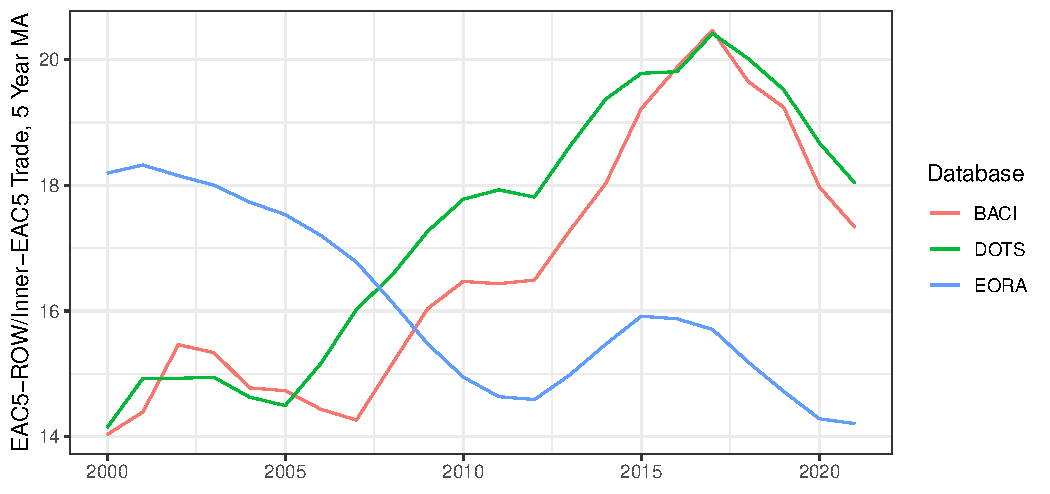
\includegraphics[width = 0.8\textwidth]{"../Figures/REV/ROW_EAC5_Trade_Ratios_5YMA.pdf"} \\
\raggedright
\scriptsize 
\emph{Notes:} Figure shows the ratio of EAC5 $\Leftrightarrow$ ROW to inner-EAC5 trade (exports + imports), smoothed using a backward-looking 5-year MA. The EAC5 includes Tanzania, Kenya, Uganda, Rwanda and Burundi.
\end{figure}
\FloatBarrier


Figure \ref{fig:GTEACshares} shows the EAC5 share in members and total EAC5 exports and imports. Uganda substantially increased the share of its exports destined to EAC5 partners, reaching 28\% in 2016 and falling again in recent years. Tanzania also increased its EAC5 export share from about 7\% in 2000 to 15\% in 2021. Kenya, on the other hand, decreased its EAC export share from 25\% in 2000 to 20\% in 2021. Rwanda shows a declining trend in both export and import share since 2012. In Burundi, the EAC5 share is constant since 2005. The total EAC5 shows a slight decline in regional export share from 2010 (18\%) to 2020 (16\%), and a clear decline in the import share from 10\% in 2000 to 7.5\% in 2020. Both shares slightly increased thereafter, consistent with Figure \ref{fig:EAC_ROW_Ratios}. The imports decline is driven by Uganda and Tanzania, while Kenya increased its EAC5 import share from 1\% in 2000 to 4\% in 2020. The aggregate pattern echoes \citet{obasaju2021regional}'s observation that the regional hegemon (Kenya) has weak backward linkages (imports) with other REC members. Also, as documented by \citet{engel2016sacu}, the hegemon has strong regional forward linkages (exports), whereas smaller economies (Rwanda, Burundi) are more regionally focused, particularly through high import shares. Over time, this pattern has weakened slightly, but trade integration has not improved in overall terms. 

\begin{figure}[h!] 
\centering
\caption{\label{fig:GTEACshares}\textsc{EAC5 Share in Members Gross Trade Flows}}
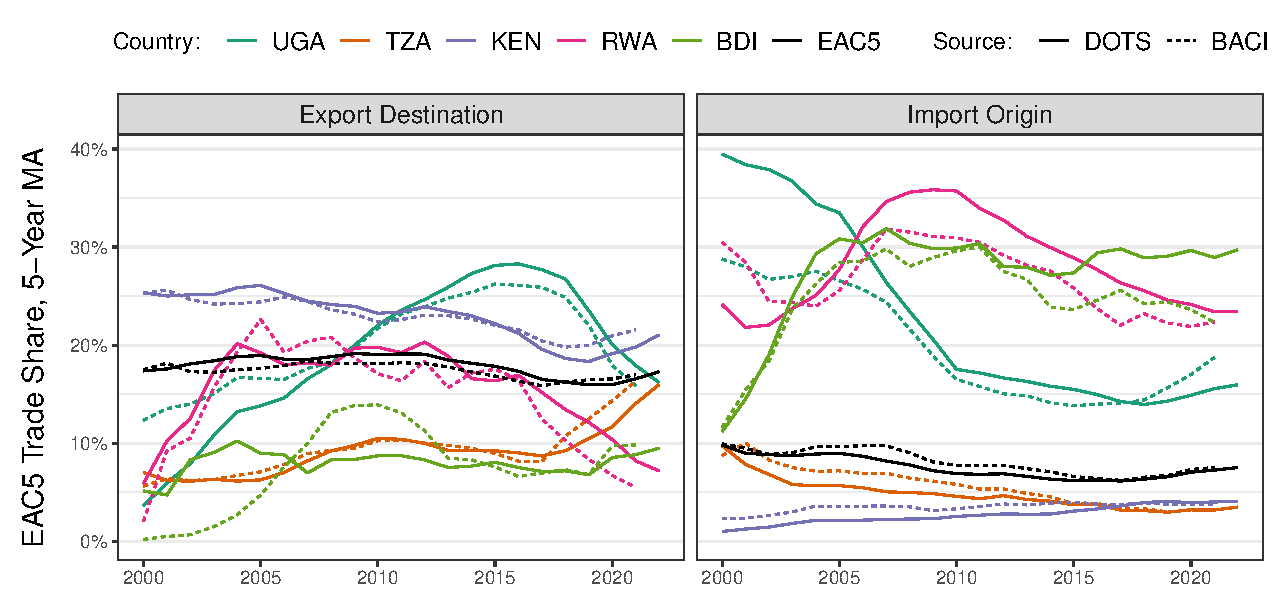
\includegraphics[width=0.9\textwidth, trim= {0 0 0 0}, clip]{"../Figures/REV/GT_EAC5_shares_ts.pdf"} \\ 
\raggedright
\scriptsize 
\emph{Notes:} Figure shows the EAC5 share in members total exports and imports, smoothed using a backward-looking 5-year MA. The black line also shows the EAC5's total share of exports and imports with itself.
\end{figure}
\FloatBarrier

When dividing trade flows broadly into agricultural products (AFF), processed foods and beverages (FBE), and manufactured goods, some further heterogeneity emerges. Figure \ref{fig:MIG_SEC_BACI} shows these flows using BACI, Appendix Figures \ref{fig:MIG_SEC_EORA} and \ref{fig:MIG_SEC_EM} using EORA and EM, respectively. \newline 

\begin{figure}[h!] 
\centering
\caption{\label{fig:MIG_SEC_BACI}\textsc{Average 2010-2019 BACI Trade Flows by Broad Sector: USD Billions}}
\vspace{2mm}
\resizebox{\textwidth}{!}{
\begin{tabular}{ccc}
Agriculture \& Livestock & Foods \& Beverages & Manufactured Goods \\
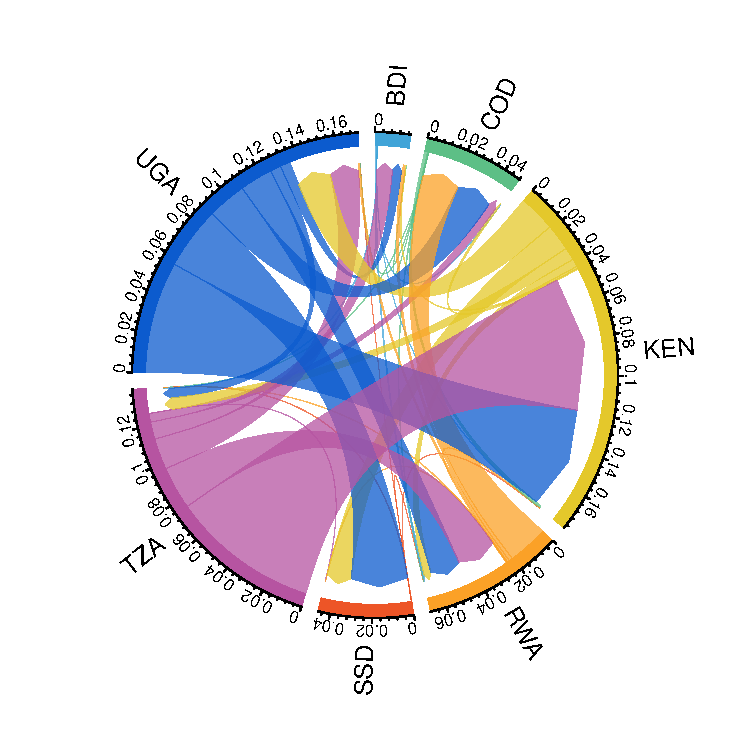
\includegraphics[width=0.4\textwidth, trim= {1.3cm 0.8cm 0.95cm 1cm}, clip]{"../Figures/REV/BACI_MIG_AGR_2010_19.pdf"} & 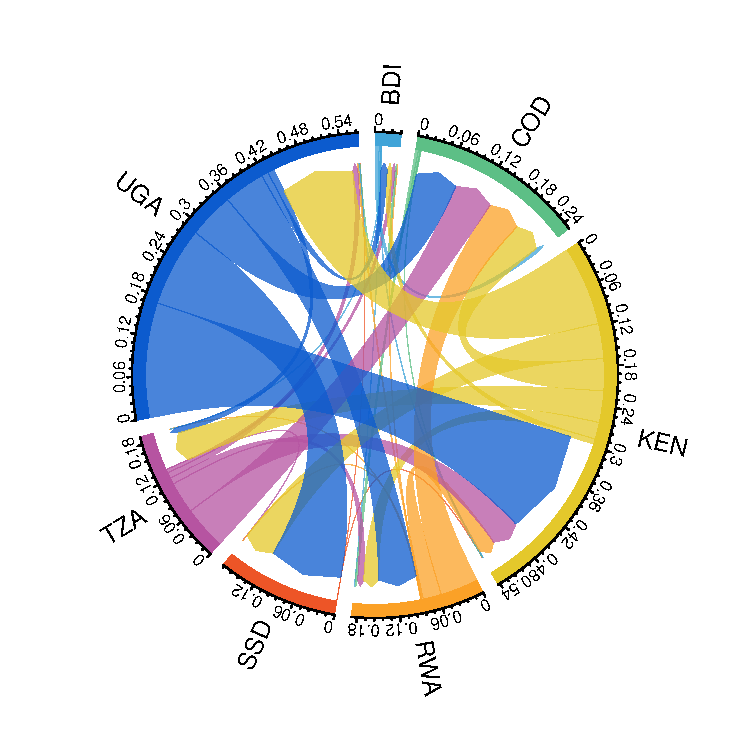
\includegraphics[width=0.4\textwidth, trim= {1.3cm 0.8cm 1cm 1cm}, clip]{"../Figures/REV/BACI_MIG_FBE_2010_19.pdf"} &
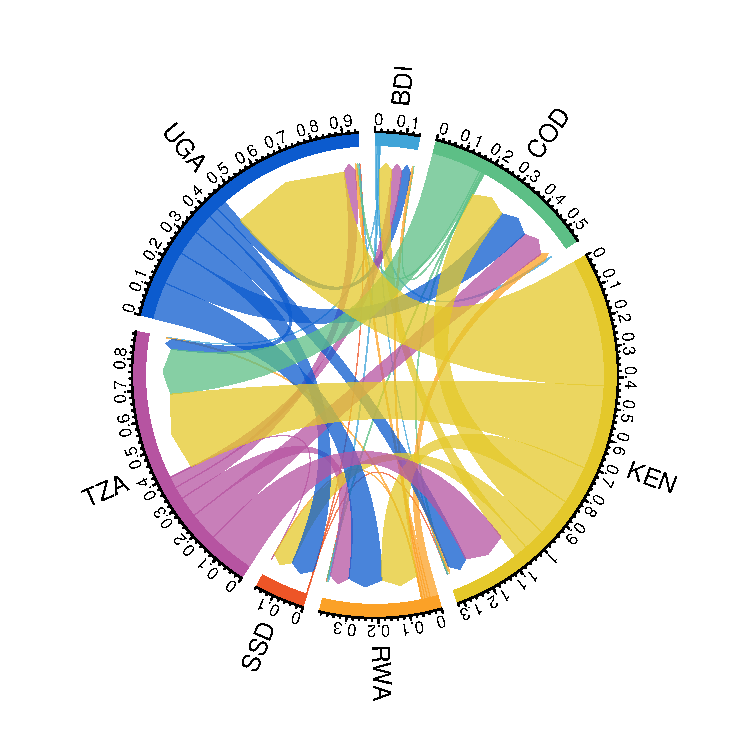
\includegraphics[width=0.4\textwidth, trim= {1.3cm 0.8cm 1.1cm 1cm}, clip]{"../Figures/REV/BACI_MIG_MAN_2010_19.pdf"} \\
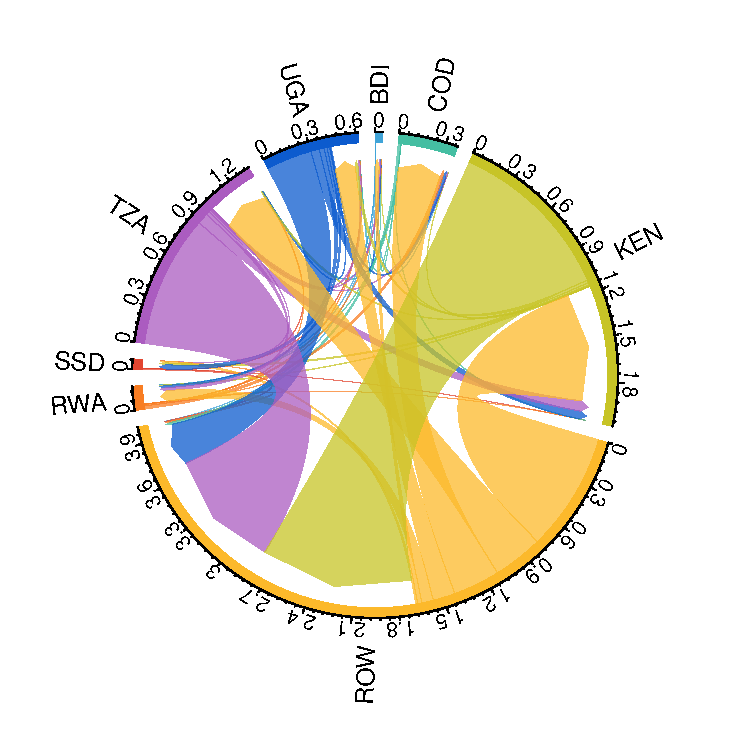
\includegraphics[width=0.4\textwidth, trim= {0.85cm 0.8cm 1.1cm 1cm}, clip]{"../Figures/REV/BACI_MIG_AGR_2010_19_ROW.pdf"} & 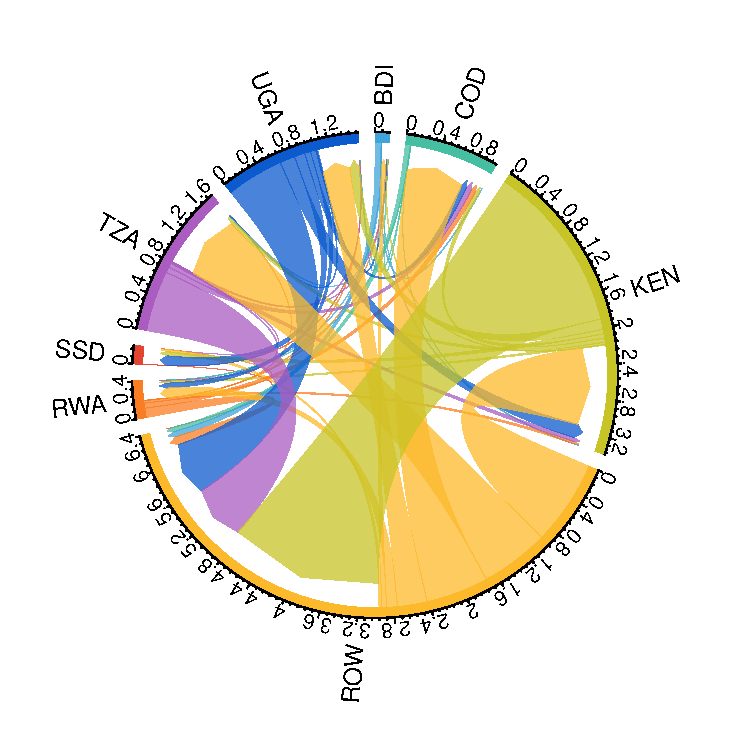
\includegraphics[width=0.4\textwidth, trim= {0.85cm 0.8cm 1.1cm 1cm}, clip]{"../Figures/REV/BACI_MIG_FBE_2010_19_ROW.pdf"} &
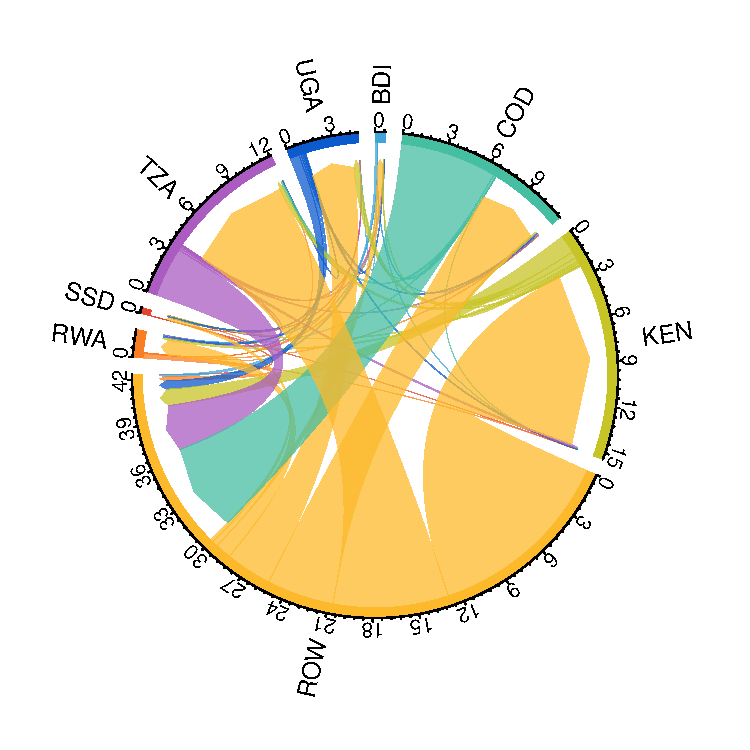
\includegraphics[width=0.4\textwidth, trim= {0.85cm 0.8cm 1cm 1cm}, clip]{"../Figures/REV/BACI_MIG_MAN_2010_19_ROW.pdf"} \\
\end{tabular}
}
\raggedright
\scriptsize 
\emph{Notes:} Figure shows the mean of bilateral gross trade flows over the years 2010-19 recorded in billions of current USD according to CEPII BACI. The top panel shows inner-EAC flows; the bottom panel includes ROW as a trading partner. The circular axis records the total flows (exports + imports) for each partner. The broad sectors shown are AFF (left), FBE (middle), and TEX-MAN (right) in Table \ref{tab:sec}. Produced using the \emph{migest} R package \citep{rmigest}.
\end{figure}
\FloatBarrier

According to all databases, Uganda and Tanzania are large regional suppliers of agricultural produce. All countries have some stakes in FBE, with Uganda supplying the most, followed by Kenya. In manufacturing, Kenya has a distinct lead, followed by Tanzania and Uganda. With ROW, all EAC countries are large agricultural exporters and importers of manufactured products. Kenya is the largest EAC supplier of both agriculture and processed foods to ROW, whereas it only plays a minor supplier role in the EAC. Tanzania supplies large amounts of gold, and Congo large amounts of minerals to ROW, which are subsumed under MPR and PCM in Table \ref{tab:sec}, making Kenya also the largest EAC exporter of manufactures. The data thus expound differences in the nature of trade both within the EAC and with ROW. Shared capacities exist for FBE, which has also been the focus of policymakers and regional studies. For example \citet{Daly2017RVCs} show that Uganda exports diary and maize produce to Kenya for processing, but has also received FDI and begun to upgrade its own food processing sector. The Ugandan Ministry of Finance and Planning \citep{EGF21}, IGC Uganda \citep{fowler2019agro} and IFPRI \citep{van2020institutional} have identified agro-industrialization as an important pillar of growth for the country. \newline


Figure \ref{fig:EAC_ROW_Ratios_Sec} shows corresponding ratios of EAC5-ROW to inner-EAC5 trade, indicating that regional trade in agriculture and, to a lesser extent, FBE, assumes increasing shares of overall EAC trade in these sectors. According to BACI, in 2020, the inner-EAC5 trade in agricultural products was 10 times smaller than EAC5-ROW trade, down from almost 40 times smaller in 2000. Similarly, FBE inner-EAC5 trade was 11 times smaller in 2020, compared to 16 times smaller in 2000. In contrast, the ratio in manufacturing shows an oscillating increase from 15 in 2000 to 20 in 2020. These developments are also reflected in the MRIO databases. \newline

\begin{figure}[h!]
\centering
\caption{\label{fig:EAC_ROW_Ratios_Sec} Gross ROW-EAC5 Trade to Inner EAC5 Trade Ratio by Broad Sector}
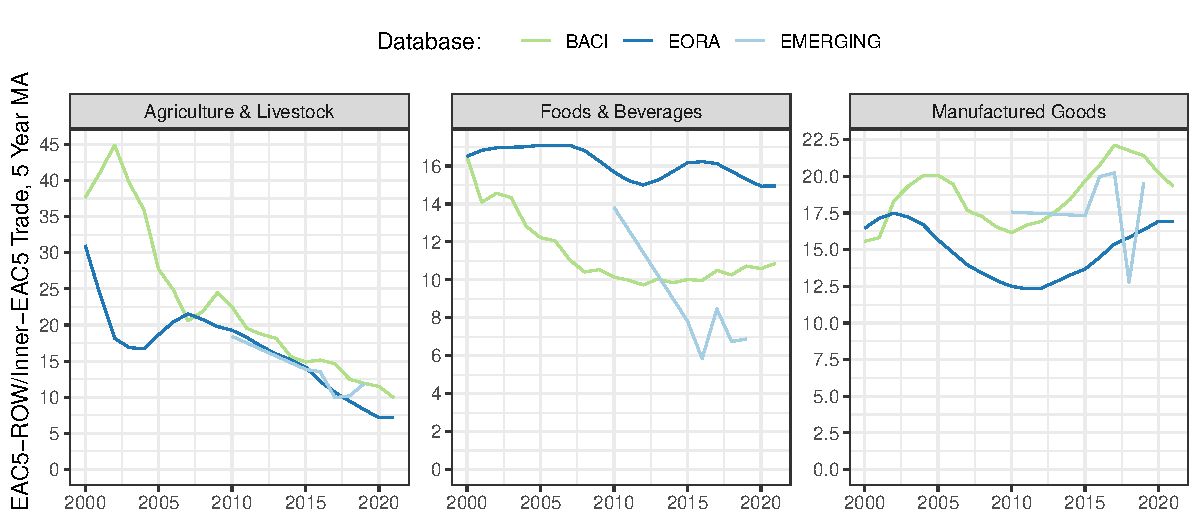
\includegraphics[width = \textwidth]{"../Figures/REV/ROW_EAC_Trade_Ratios_Sec_5YMA.pdf"}
\raggedright
\scriptsize 
\emph{Notes:} Figure shows the ratio of EAC5 $\Leftrightarrow$ ROW to inner-EAC5 trade (exports + imports), smoothed using a backward-looking 5-year MA. The EAC5 includes Tanzania, Kenya, Uganda, Rwanda and Burundi. The broad sectors shown are AFF (left), FBE (middle), and TEX-MAN (right) in Table \ref{tab:sec}.
\end{figure}

Figure \ref{fig:GTEACsharesSec} again provides a detailed breakdown by exports/imports and individual members. In agriculture, export and import shares both increased: in 2015-20, the EAC5 exported 12.6\% of agricultural exports to itself, up from 4.6\% in 1995-2000, and imported 19.3\%, up from 9.3\% in 1995-2000. The FBE export shares also rose from 7.8\% to 13.7\%, whereas the import share remained constant around 20\%. In manufacturing, the opposite is the case, with the EAC5 exports share declining from 32\% to 18.6\% and the import share remaining roughly constant at around 7\%. At the country level, Uganda significantly increased its EAC5 share as an exporter and importer of both agricultural produce and FBE. This development is mirrored, to a lesser extent, by Kenya, which additionally maintains a very high EAC5 share in manufactured exports of around 40\%, down from nearly 50\% in 2000. This stands in stark contrast to a very small EAC5 import share of less than 1\%. Tanzania increased its export share to the EAC5 in all 3 broad sectors while further decreasing its already low import shares in foods and manufactures to around 5\%. Rwanda and Burundi have high export and import EAC5 shares in all sectors apart from manufacturing exports. Rwanda strongly decreased its EAC5 agriculture and foods export shares since 2007, approaching the levels of Kenya in 2020, whereas Burundi strongly increased its agricultural export share from almost 0\% in 2005 to 60\% in 2020, while decreasing its import share from 70\% to 30\%. \newline 

\begin{figure}[h!] 
\centering
\caption{\label{fig:GTEACsharesSec}\textsc{EAC5 Share in Members Gross Trade by Sector using BACI Data}}
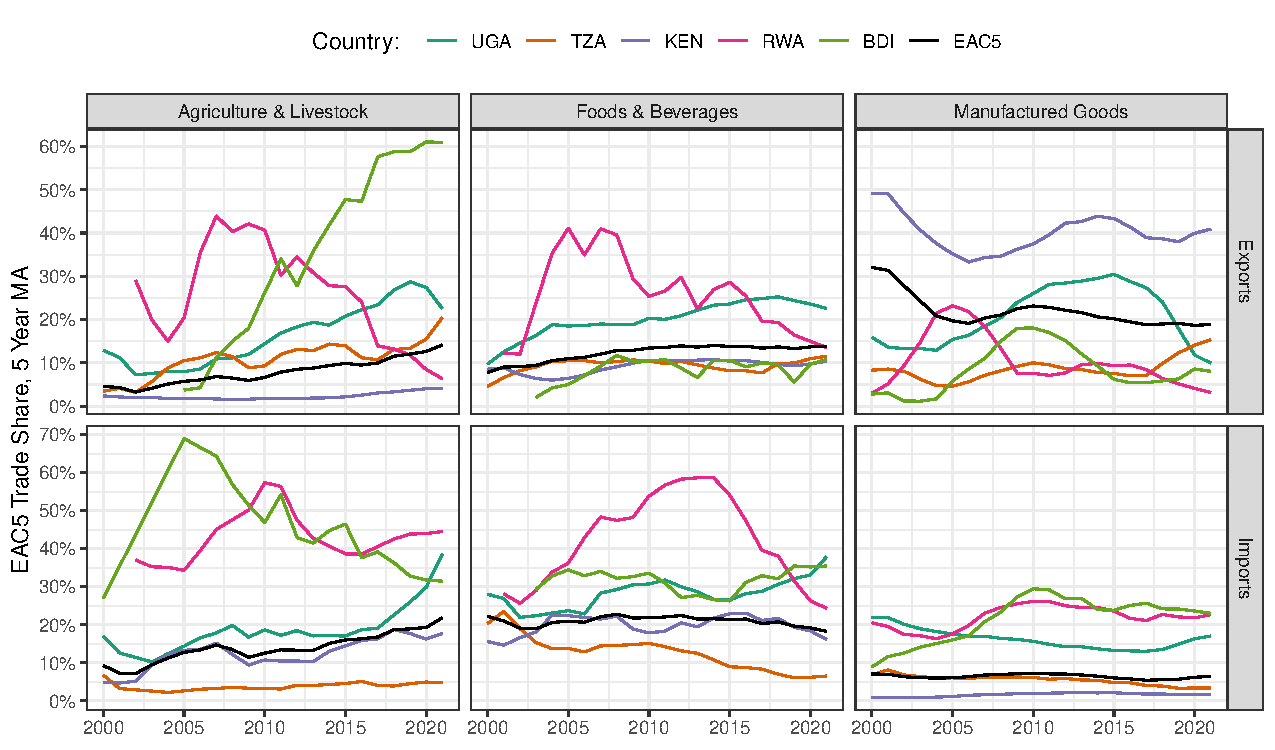
\includegraphics[width=\textwidth, trim= {0 0 0 0}, clip]{"../Figures/REV/GT_EAC5_shares_sec_ts.pdf"} \raggedright
\scriptsize 
\emph{Notes:} Figure shows the EAC5 share in members' total exports and imports, smoothed using a backward-looking 5-year MA. The broad sectors shown are AFF (left), FBE (middle), and TEX-MAN (right) in Table \ref{tab:sec}.
\end{figure}
\FloatBarrier

Considering their different levels of development, this suggests that countries first become regional agricultural exporters and later suppliers of manufactured goods. However, it seems like these manufactures do not cater very well to other members' demands, as evidenced by the declining EAC5 shares in both exports and imports, and thus fail to become a driver of regional integration. The hegemonic position of Kenya as a supplier of manufactures may also crowd out other countries' attempts to increase their regional supply. Thus, gross trade data suggests that EAC regional integration through trade is asymmetric, has progressed mainly via agriculture and FBE, and is stronger in exports. Particularly, the larger economies of Tanzania and Kenya import much more from ROW. Among the EAC5, Tanzania is overall least integrated into regional trading. 

\subsection{Intermediate Flows}

An advantage of MRIO databases is that they record gross trade in both intermediates and final goods. Due to its greater accuracy, I only examine such flows using the EM database, averaged across 2015-2019 to smooth temporal variation. Figure \ref{fig:wld} provides an aggregate intermediate flows table. The columns indicate intermediate inputs required by each country or region from each row country or region. Conversely, the rows indicate intermediate quantities supplied. \newline  

Among the EAC countries, the table shows a significant supplier role of Kenya, supplying $10^{2.72} = 524$ million USD to Uganda, $10^{2.22} = 168$ million USD to Tanzania and  $10^{1.96} = 91$ million USD to Rwanda. Uganda/Tanzania also supplies 258/228 million to Kenya and 90/70 million to Rwanda. Tanzania supplies 56 million to Uganda, Rwanda 54 million to Kenya, and all other inner-EAC intermediate trade is below 35 million.\footnote{Exempting South Sudan, subsumed in SSA because of data quality concerns, which receives 385 million in intermediates from Uganda and 223 million from Kenya.} EM estimates intermediate trade with ROW to be 27.3 times greater than inner-EAC trade, composed of intermediate inputs from ROW summing to 15.6 times EAC intermediates trade and EAC inputs to ROW summing to 11.8 times EAC intermediates trade. The largest supplier of intermediates is China, supplying 831m to Uganda, 1937m to Tanzania, and 2704m to Kenya, followed by South Asia supplying 601/1066/1562, respectively, and the EU supplying 620/844/1462. Compared with these, the rest of SSA is relatively insignificant at 184/325/514. In terms of demand for EAC intermediates, the EU is the largest importer, importing 552/828/1402, followed by the Middle East and North Africa (769/352/503), South Asia (101/683/618), the rest of SSA (105/716/462) and China (148/631/340). China, notably, supplies 4.9 times more intermediates than it demands from these three economies. The supply and demand of intermediates with the EU, NAC, and SSA are quite balanced. Overall, Uganda, Tanzania, and Kenya combined demand 1.7 times more inputs from ROW than they supply. It should be noted that Congo, while not really integrated with other EAC members in terms of intermediates, has large and surprisingly balanced intermediate flows with ROW, demanding/supplying 2598/2636 with the EU and 1199/1375 with China. 

\begin{figure}[h!] 
\centering
\caption{\label{fig:wld}\textsc{Aggregated EMERGING MRIO Table: 2015-2019 Average}}
\small{\textit{Log10 Millions of Current USD at Basic Prices}}
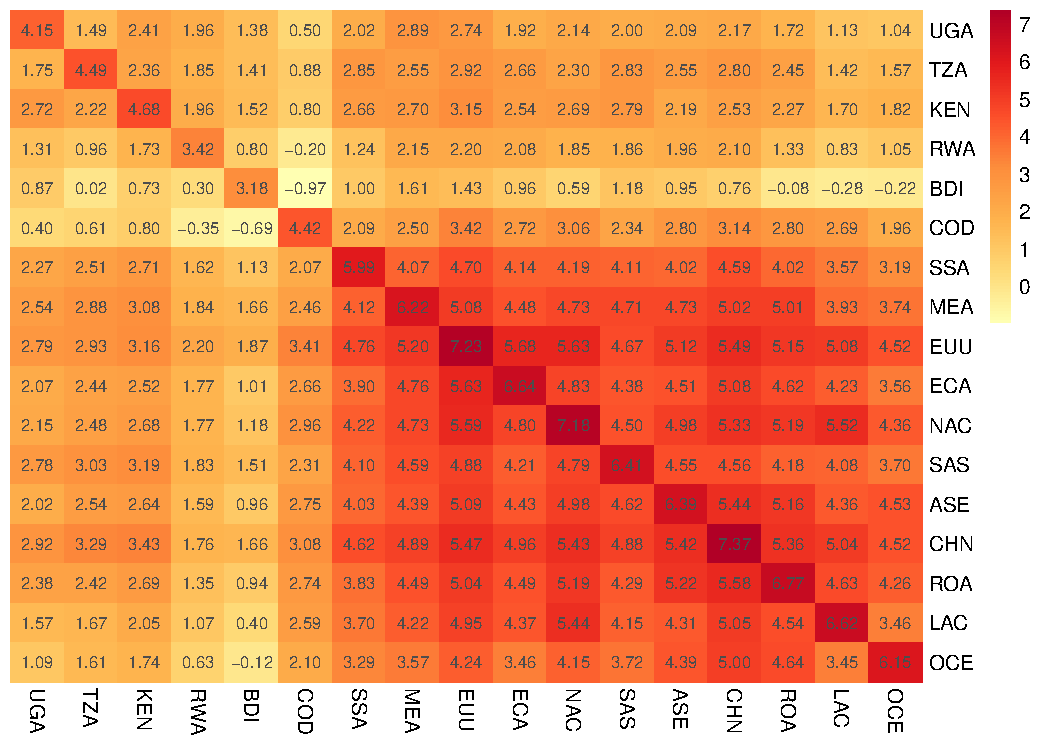
\includegraphics[width=1\textwidth, trim= {0 0 0 0}, clip]{"../Figures/REV/EM_heatmap_2015_19_AG.pdf"} \\ 
\raggedright
\scriptsize
\emph{Notes:} Figure shows gross intermediate input flows in log10 USD millions. Rows indicate the sources, and columns the destinations of intermediates. The diagonal sums the domestic IO/regional ICIO table. 
\end{figure}
\FloatBarrier

Despite its high use of foreign inputs, domestic intermediate inputs corresponding to the diagonal entries are, on average, 4.1 times greater than foreign inputs in EAC countries and 6.3 times greater than EAC inputs to other countries. For the region as a whole, these figures are 4.6 and 6.13, respectively. This is low compared to other major regions, which produce and trade a lot more within themselves. For example, in the EU and North America, own inputs are around 10 times greater than foreign inputs. For China, it is 14 times. \newline

To provide some sector-level detail, Appendix Table \ref{tab:weaclfl} records the 50 largest sector-level intermediate flows (excl. Congo). Both with ROW and inside the EAC, the largest intermediate flows are in manufacturing and, in particular, in petrochemicals (PCM), FBE, and, to a lesser extent, textiles (TEX). Kenya is a significant EAC supplier of manufacturing inputs, particularly for PCM, FBE, and metal product (MPR) industries. Kenya also supplies large transport (TRA) (including travel and tourism) intermediates to EU TRA services and agricultural inputs to EU FBE industries. It also supplies large inputs for FBE industries in South Asia. These flows are, on average, 3-4 times larger than its regional intermediate supplies. Uganda supplies PCM to ROW, and FBE and agriculture to Kenyan FBE and TRA industries. 


\subsection{Aggregate Structure of Production and Trade}

Figure \ref{fig:shares_ag} compactly summarizes the structure of production and trade in the EAC. VA is around 60\% of output in all EAC members, apart from Rwanda, where it is 73\%. The other components of output are domestic and imported intermediates, of which, as the second plot shows, between 17 and 24\% are imported by different EAC members. Gross output is then either consumed or exported for either intermediate or final use. The RHS of Figure \ref{fig:shares_ag} shows that between 5 and 16\% of gross output is exported by EAC members. 

\begin{figure}[h!] 
\centering
\caption{\label{fig:shares_ag}\textsc{Gross Decomposition of EAC Production and Trade}}
\vspace{2mm}
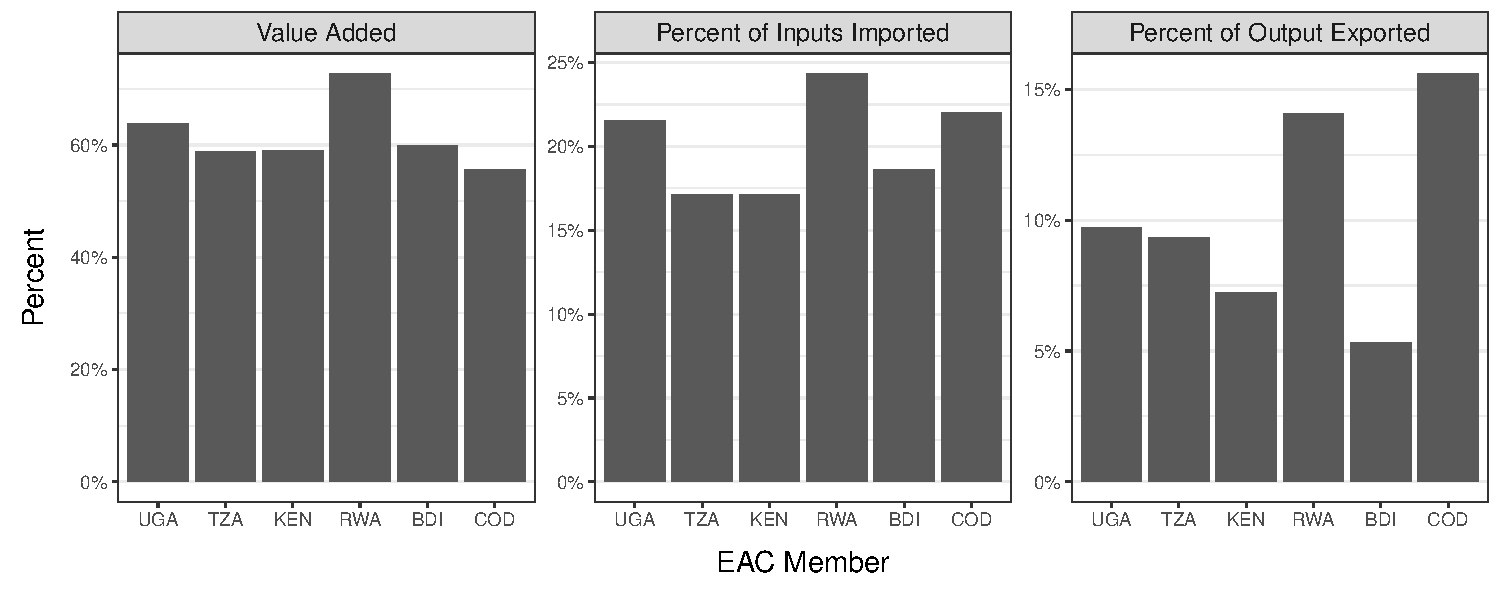
\includegraphics[width=1\textwidth, trim= {0 1cm 0 0}, clip]{"../Figures/REV/EM_gross_shares_ag.pdf"} 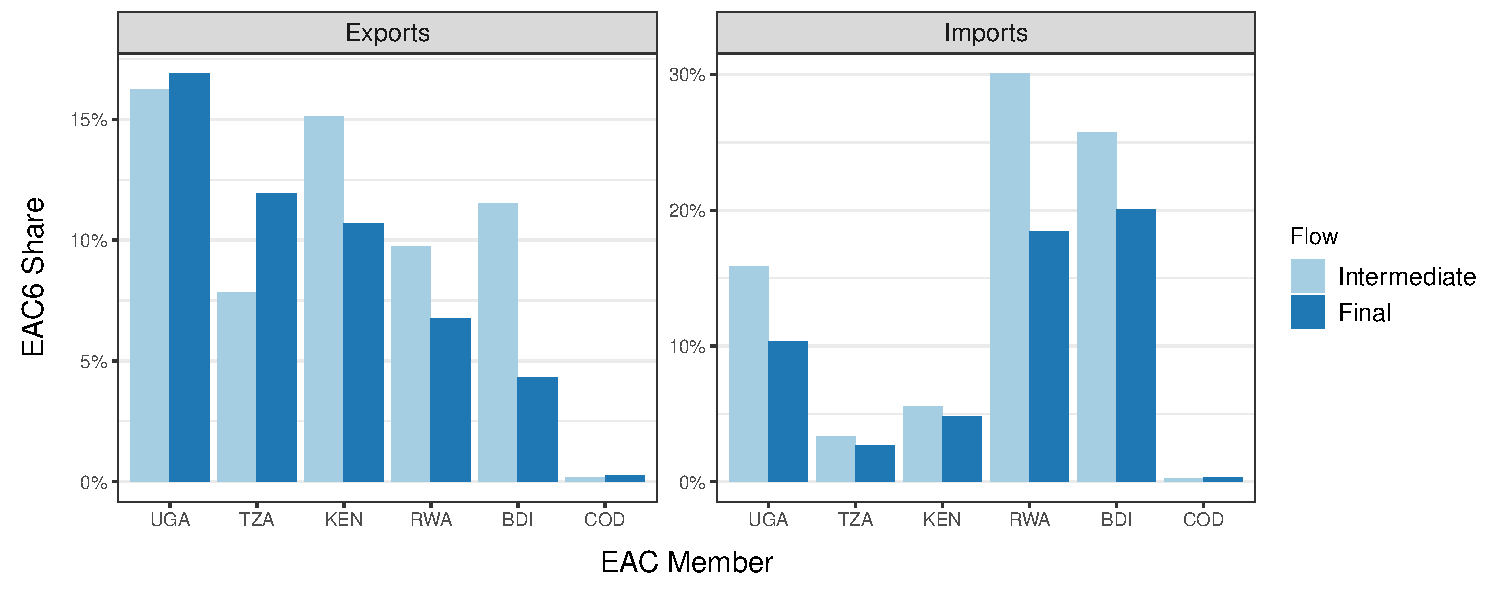
\includegraphics[width=1\textwidth, trim= {0 0 0 0}, clip]{"../Figures/REV/EM_gross_trade_shares_ag.pdf"} \\
\raggedright
\scriptsize
\emph{Notes:} Based on EMERGING and computed using an 2015-2019 average MRIO table. 
\end{figure}
\FloatBarrier

The bottom panel of Figure \ref{fig:shares_ag} decomposes exports and imports by type of flow. It shows that Uganda, Rwanda, and Burundi have significant export and import shares with the EAC for both intermediate and final products. Kenya and Tanzania, on the other hand, export significant amounts to the EAC but only import small shares. With the exception of Tanzanian and Ugandan exports, inner-EAC trade in intermediates is slightly larger than trade in final goods. 



\section{Value Chains}

While gross intermediate flows provide useful information about direct productive relationships, they do not reveal how much of the value was added in the supplying country-industry and previous production stages performed by other country-industries. The Leontief decomposition solves this problem by reallocating the value of intermediate inputs to the original producers \citep{Kummritz2014}. To guide the further discussion of VA trade flows, I begin with some formal derivations and introduce a consistent notation used throughout this paper. \newline

Let $\textbf{A}$ be a normalized ICIO table where each element $a_{oi,uj}$ gives the units of origin country $o$ and sector $i$'s (row) output required for the production of one unit of using country $u$ and sector $j$'s (column) output, $\textbf{x}$ the vector of outputs of each country-sector, and $\textbf{d}$ a vector of final demand (FD) such that the following productive relationship holds
%
\begin{equation} \label{eq:io_model}
\textbf{x} = \textbf{A}\textbf{x} + \textbf{d}.
\end{equation}
%
\citet{leontief1936quantitative}'s insight was that one could solve this equation for $\textbf{x}$ to get the amount of output each country-sector should produce given a certain amount of FD
%
\begin{equation} \label{eq:leontief}
\textbf{x} = (\textbf{I}-\textbf{A})^{-1} \textbf{d} = \textbf{B}\textbf{d},
\end{equation}
%
\noindent where the Leontief Inverse in denoted $\textbf{B} = (\textbf{I}-\textbf{A})^{-1}$. This matrix is also often called the total requirement matrix since it gives the total productive input requirement from each sector to produce one unit of final output\footnote{Specifically each element in $b_{oi,uj}$ in \textbf{B} gives the output required from country-sector $oi$ for the production of one unit of the final good in $uj$. Thus, the first column of \textbf{B} gives all the productive input required from all sectors for the production of one unit of the final good in sector 1, and the first row of \textbf{B} gives all the input required from sector 1 to produce one unit of the final good in each sector. \vspace{-5mm}}. The direct VA share of each country-sector is given by
%
\begin{equation}
\textbf{v} = \textbf{1} - \textbf{A}'\textbf{1},
\end{equation}
%
where $\textbf{1} = (1, 1, 1, ..., 1)'$ is a column-vector of 1's. Let \textbf{V} be the matrix with \textbf{v} along the diagonal and 0's in the off-diagonal elements. Multiplying Eq. \ref{eq:leontief} with $\textbf{V}$ then gives VA in each country-sector
%
\begin{equation} \label{eq:VB}
\textbf{V}\textbf{x} = \textbf{V}(\textbf{I}-\textbf{A})^{-1} \textbf{d} = \textbf{VBd}.
\end{equation}
%
The term $\textbf{VB} = \textbf{V}(\textbf{I}-\textbf{A})^{-1}$ is known as the matrix of VA multipliers or VA shares, which can be used to obtain the amount of VA generated in each sector (\textbf{Vx}) when producing to satisfy FD (\textbf{d}). More specifically, the matrix $\textbf{VB}$ contains the amount of VA by each country-sector (row) to the production of one unit of each country-sector's (column's) output. 


\subsection{Backward GVC Participation}

The FVA share in domestic production and exports, termed 'Vertical Specialization' (VS) by \citet{hummels2001nature}, is the most widely used measure of backward GVC integration. Consider \textbf{VB} with elements vb$_{oi,uj}$, then VS for a particular country-sector may be expressed as
%
\begin{equation} \label{eq:VS}
\text{VS}_{uj} = \sum_{oi,\ o \neq  u} \text{vb}_{oi, uj}\ \ \forall uj.
\end{equation}
%
Figure \ref{fig:EACVB_ag_ts} shows a time series of VS according to different data sources. The calculated VS measure using EORA21 is identical to the WDR one. The extension of EORA through 2021, as mentioned, introduces a large structural break in 2016, which, in some cases such as Tanzania where VS drops to zero or Burundi where VS rises to above 50\% (truncated in Figure \ref{fig:EACVB_ag_ts}) is highly unrealistic. EM is the more reliable database for these countries and indicates that for all EAC members, between 8\% and 30\% of production/exports is foreign content. Furthermore, EM suggests that the smaller economies Burundi, Rwanda, and Uganda have increased their VS, especially in 2015-2019, whereas Kenya and Congo have seen a decline in VS. In Tanzania, VS appears stagnant at $\sim$16\%. 

\begin{figure}[h!] 
\centering
\caption{\label{fig:EACVB_ag_ts}\textsc{EAC Backward GVC Participation}}
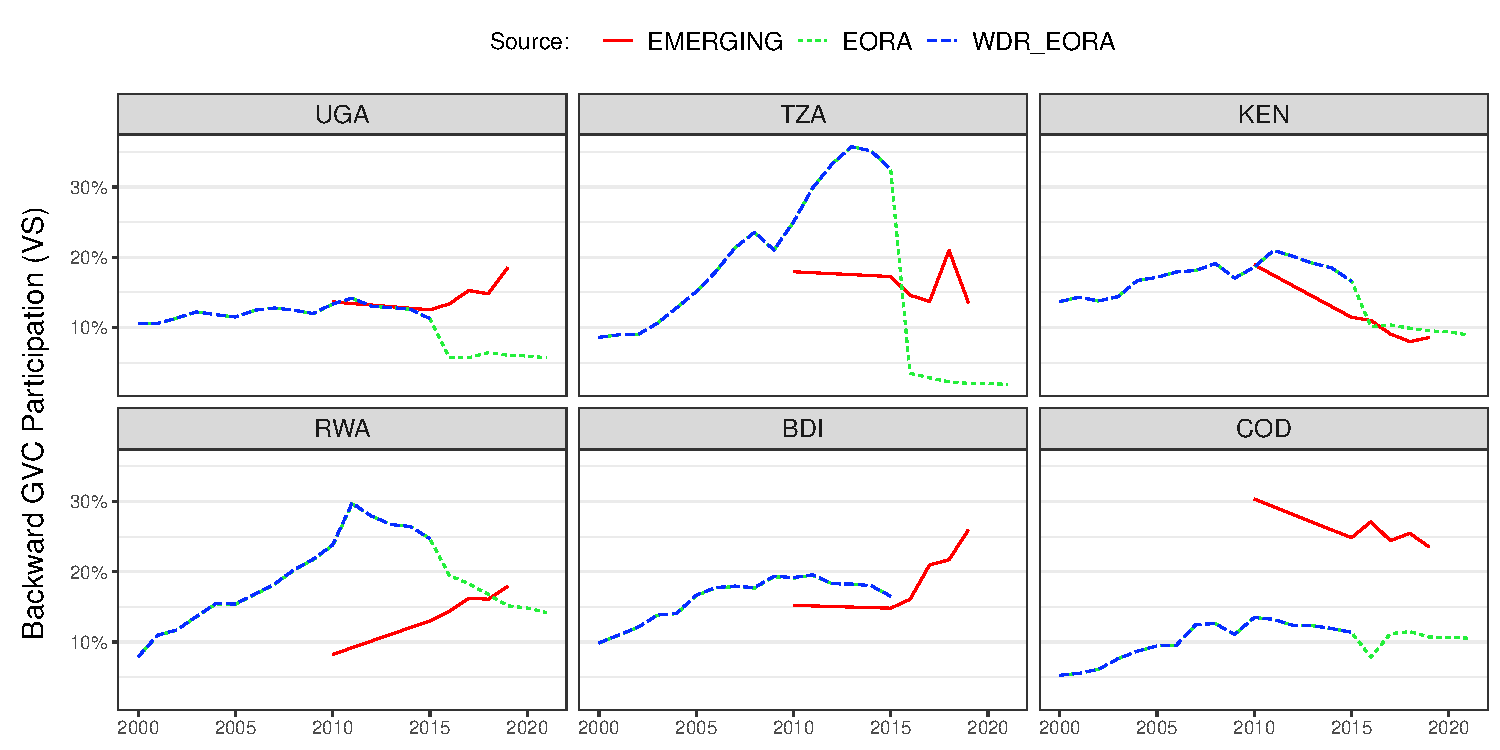
\includegraphics[width=1\textwidth, trim= {0 0 0 0}, clip]{"../Figures/REV/VA_shares_ag_ts.pdf"} \raggedright
\scriptsize
\emph{Notes:} \citet{hummels2001nature}'s index of Vertical Specialization (VS) is the FVA share in gross output and exports. 
\end{figure}
\FloatBarrier

Apart from its overall size, the composition of VS is of interest. Figure \ref{fig:EACVB_ctry} shows a breakdown of VS by source country/region, averaged, for EORA between 2010 and 2015 and for EM between 2015 and 2019. Congruent to the EAC import share shown in the bottom right panel of Figure \ref{fig:shares_ag}, only Rwanda, Burundi, and Uganda source a significant fraction of foreign inputs from EAC partners. According to EM, Kenya supplies 11.5\% of the foreign content in Ugandan exports, 9.8\% in Rwanda, and 8\% in Burundi. Uganda also supplies 9.3\% of the foreign content in Rwandan exports and 5.5\% in Burundi. In absolute values, Uganda supplies slightly more to Kenyan export production (around 23 million USD according to EM, vs. 20.7 million to Rwanda). This is dwarfed by the 115 million that Kenya adds to Ugandan exports. \newline 

In total, the EU and China have the greatest shares in EAC VS. The EU supplies 33\% of the foreign content of Congolese exports, 23\% in Burundi, 21\% in Rwanda, 17\%, 16\%, 15\% in Uganda, Kenya, and Tanzania, respectively. China supplies 27\% of the foreign content of Kenyan and Tanzanian exports (approx. 300 million USD in both cases), 21\% in Uganda, and 16\% in Congo. Thus, overall, EAC exports have modest amounts of foreign content, and most of this VS, particularly for major exporters Congo, Kenya, and Tanzania, originates in the EU or China. 


\begin{figure}[h!]
\centering
\caption{\label{fig:EACVB_ctry}\textsc{EAC Backward GVC Participation: Sources of Foreign Content}}
\small{\textit{Average EMERGING 2015-2019 Foreign Content Share in Parentheses}}
\vspace{2mm}
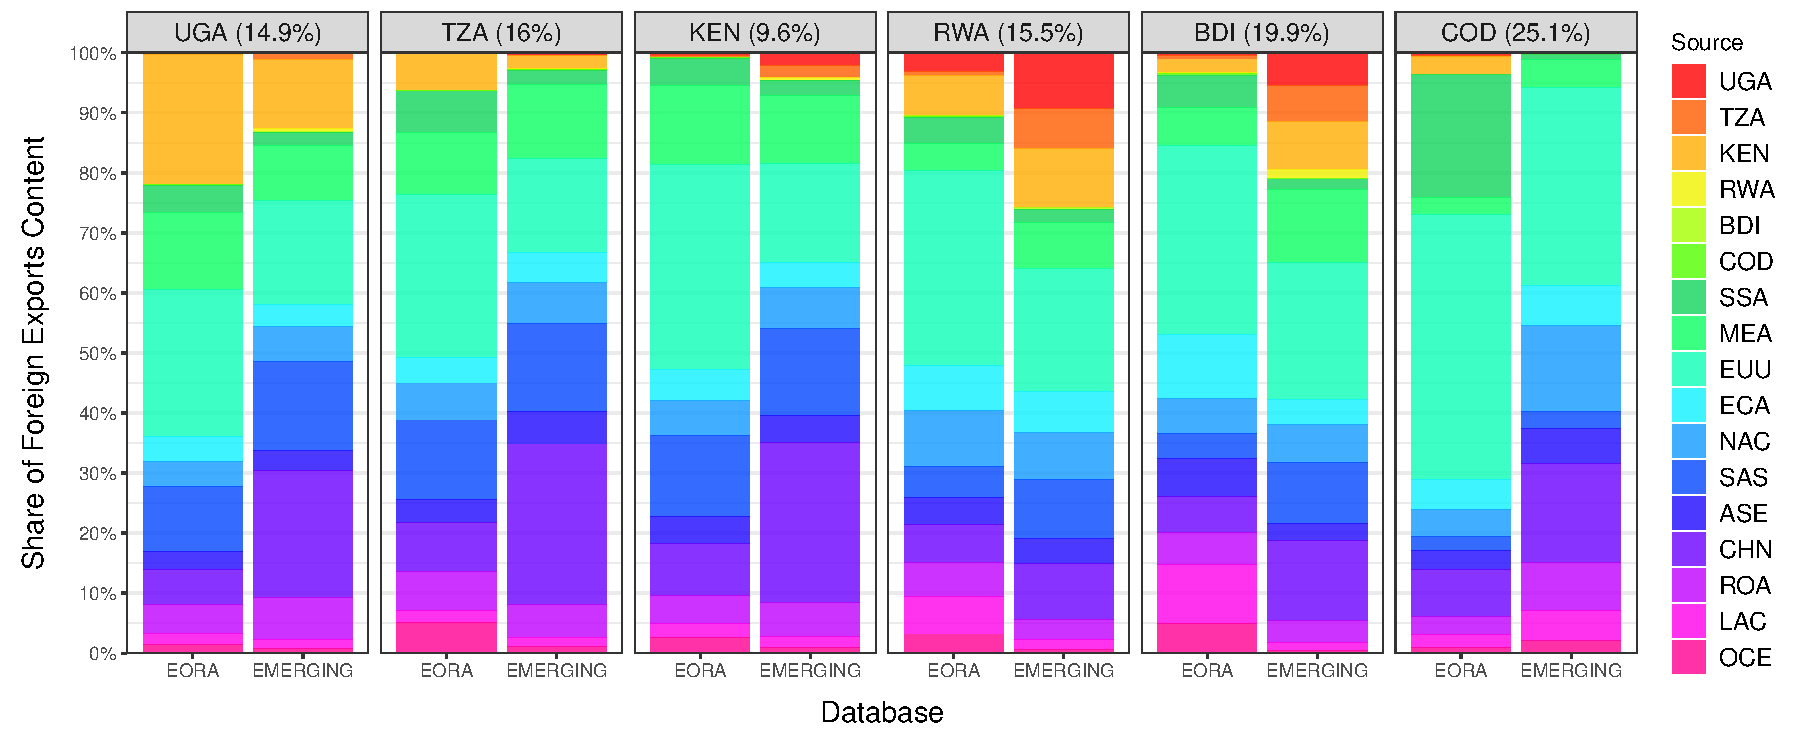
\includegraphics[width=1\textwidth, trim= {0 2mm 0 0}, clip]{"../Figures/REV/VA_shares_ctry.pdf"} \\ \raggedright
\scriptsize
\vspace{-2mm}
\emph{Notes:} Figure shows a breakdown of VS by source country according to EORA (2010-2015) and EM (2015-2019) averages. 
\end{figure}
\FloatBarrier

Sectors exhibit great heterogeneity, both in terms of overall foreign content and its composition. Table \ref{tab:EACVB_sec} shows overall VS content shares according to EM. In general, manufacturing sectors have higher foreign content, a pattern emphasized in the WDR, which also notes that a handful of sectors, including electrical machinery (ELM) and transport equipment (TEQ), have driven GVC expansion since 1995. In the average EAC country, these manufacturing sectors have more than 20\% foreign content, but there is marked heterogeneity across countries. Notably, in Rwanda, manufacturing sectors have less than 15\% foreign content. The highest foreign content sectors by country are ELM in Tanzania (42\%), wood and paper (WAP) in Kenya (40\%), mining (MIN) and textiles (TEX) in Uganda (29\%), sales and repairs (SMH) in Rwanda (25\%), petrochemicals (PCM) in Burundi (47\%) and TEQ in Congo (36\%). Since Burundi and Congo have no IO table, these figures need to be taken with caution. The final columns of Table \ref{tab:EACVB_sec} give FVA in overall sectoral exports by EAC members, including value addition by other members, with and without Congo. These resemble a classical VS distribution centering around ELM and TEQ at $\sim$ 35\%. \newline

\begin{table}[ht!] 
\centering
\caption{\label{tab:EACVB_sec}\textsc{EAC Backward GVC Participation: Sectoral Heterogeneity}}
\small{\textit{Average EMERGING 2015-2019 Foreign Content Shares (\%)}} \\
\vspace{1mm}
\begin{tabular}{lrrrrrrrrrr}
  \toprule
sector & UGA & TZA & KEN & RWA & BDI & COD & Mean & Median & EAC6 & EAC5 \\ 
  \midrule
AFF & 5.9 & 4.1 & 3.7 & 5.8 & 15.2 & 3.3 & 6.3 & 5.0 & 4.2 & 4.4\\ 
  MIN & 29.2 & 5.5 & 0.0 & 2.0 & 17.0 & 4.7 & 9.7 & 5.1 & 4.6 & 6.8\\ 
  FBE & 22.7 & 7.6 & 3.1 & 20.6 & 19.3 & 13.6 & 14.5 & 16.4 & 11.1 & 10.7\\ 
  TEX & 29.6 & 17.1 & 25.2 & 8.3 & 8.5 & 28.6 & 19.6 & 21.2 & 26.1 & 24.1\\ 
  WAP & 13.7 & 22.7 & 39.5 & 1.4 & 5.9 & 20.1 & 17.2 & 16.9 & 24.8 & 29.2\\ 
  PCM & 23.9 & 19.8 & 19.5 & 10.2 & 47.1 & 20.6 & 23.5 & 20.2 & 20.0 & 19.7\\ 
  MPR & 27.0 & 26.9 & 16.2 & 10.2 & 39.7 & 25.0 & 24.2 & 26.0 & 24.3 & 23.6\\ 
  ELM & 18.7 & 41.9 & 30.7 & 5.2 & 27.4 & 34.9 & 26.5 & 29.1 & 34.9 & 35.2\\ 
  TEQ & 22.7 & 17.1 & 19.7 & 0.0 & 32.8 & 36.4 & 21.4 & 21.2 & 34.6 & 23.9\\ 
  MAN & 23.3 & 21.8 & 27.3 & 0.8 & 0.4 & 24.5 & 16.3 & 22.6 & 25.3 & 25.6\\ 
  EGW & 28.2 & 3.1 & 26.2 & 0.0 &  & 2.1 & 11.9 & 3.1 & 16.9 & 27.1\\ 
  CON & 15.6 & 13.1 & 16.2 & 7.4 & 5.3 & 30.6 & 14.7 & 14.3 & 12.9 & 12.9\\ 
  SMH & 5.6 & 11.7 & 9.4 & 25.2 & 14.1 & 15.3 & 13.5 & 12.9 & 10.9 & 10.9\\ 
  TRA & 7.6 & 18.5 & 6.6 & 4.7 & 0.1 & 4.3 & 7.0 & 5.7 & 11.0 & 11.0\\ 
  PTE & 11.0 & 21.7 & 5.4 & 0.0 & 0.0 & 2.5 & 6.8 & 4.0 & 11.9 & 12.0\\ 
  FIB & 0.4 & 8.2 & 0.3 & 1.9 & 0.0 & 4.5 & 2.5 & 1.1 & 1.1 & 0.9\\ 
  PAO & 5.0 & 2.2 & 8.0 & 0.0 & 0.0 & 4.5 & 3.3 & 3.4 & 6.8 & 7.0\\ 
   \bottomrule  \\ [-0.9em]
\multicolumn{11}{l}{\parbox{0.85\textwidth}{\scriptsize
\textit{Notes:} Table reports total foreign content shares (VS) according to the EM 2015-2019 average in percentage terms. These shares are reported for each EAC6 country and for the EAC6 and EAC5 as a whole, which also counts VA by members among each other as FVA, i.e., these are export-weighted averages of individual members VS. The 'Mean' and 'Median' give unweighted EAC6 averages.}}
\end{tabular}
\end{table}
% \FloatBarrier

 Figure \ref{fig:EACVB_ctry_sec} breaks down the origin of total EAC5 VS and thus provides a sector-level perspective of EAC regional integration. The sectors with the highest EAC5 share are SMH at 14.5\% and FBE at 14\%. Other sectors with sizeable regional shares are PCM at 8.6\%, TEX at 7.4\%, AFF at 7.2\%, electricity (EGW) at 6.3\% and TEQ at 6.2\%. This quantitatively highlights the potential of the FBE sector for regional integration but also indicates a failure of regional integration in many core manufacturing sectors. For example, ELM, which has a VS of around 35\% according to Table \ref{tab:EACVB_sec}, only has a 2.8\% regional share. Multiplying these percentages yields that only 1\% of the gross exports (and output) in EAC ELM is regional FVA, compared to 1.5\% for FBE. \footnote{Due to the lower FVA share of 11\% in the FBE sector. \vspace{-3mm}} Figure \ref{fig:EACVB_ctry_sec} thus indicates great potential and challenges in developing regional manufacturing value chains. 

\begin{figure}[h!] 
\centering
\caption{\label{fig:EACVB_ctry_sec}\textsc{EAC5 Backward GVC Participation: Sources of VS by Sector}}
\small{\textit{Based on Average EMERGING 2015-2019 EAC Exports (Excl. Congo)}}
\vspace{2mm}
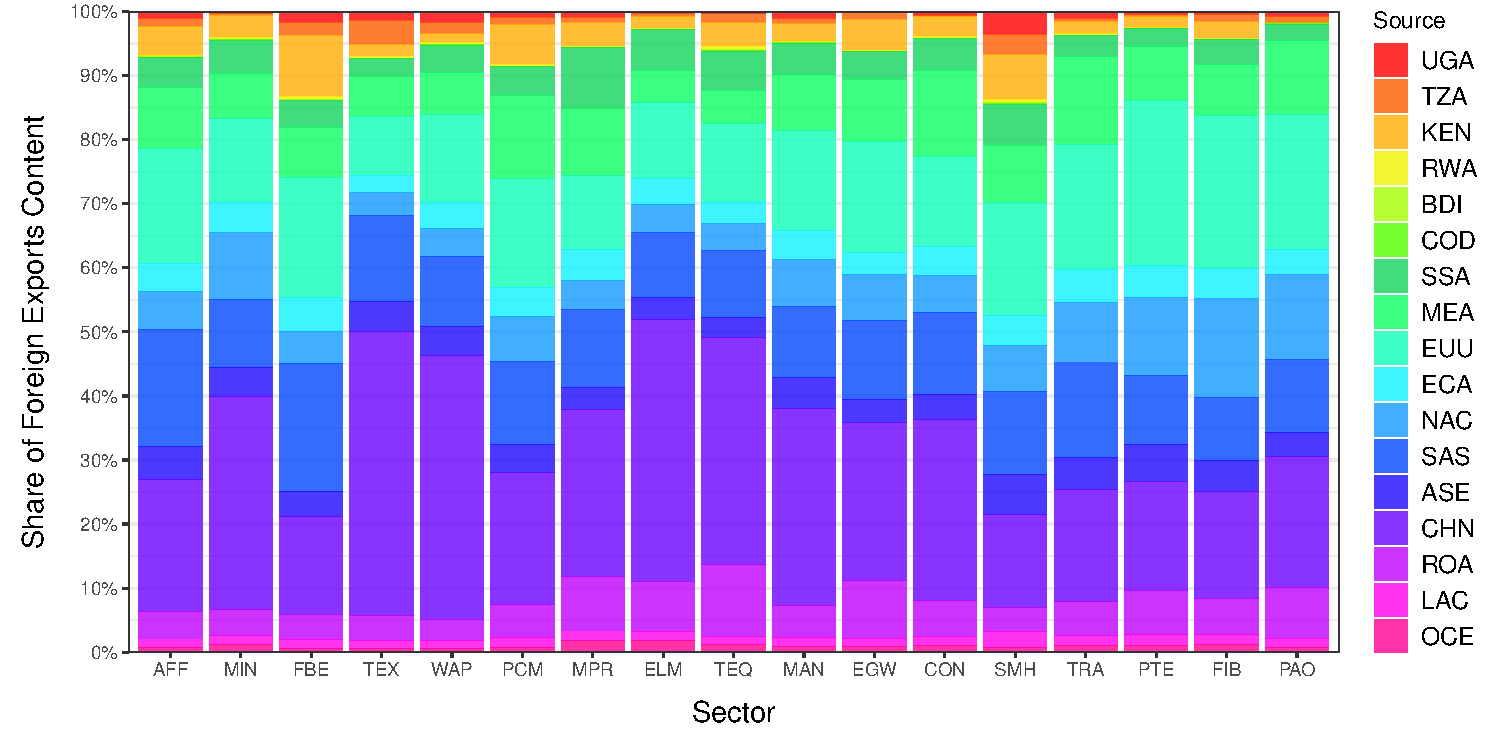
\includegraphics[width=1\textwidth, trim= {0 0 0 0}, clip]{"../Figures/REV/VA_shares_sec_ctry.pdf"} \\ 
\raggedright
\scriptsize
\vspace{-3mm}
\emph{Notes:} Figure shows a sector-level breakdown of total EAC5 VS by source country, according to EM (2015-2019) averages. 
\end{figure}
\FloatBarrier 




\subsection{Forward GVC Participation}

Apart from VS, which measures backward GVC integration, \citet{hummels2001nature}, and more formally \citet{daudin2011produces}, introduced the share of domestic exports that enter foreign countries' exports, termed VS1, as a measure of forward GVC Integration. It is defined as\footnote{For completeness I note that VS can be defined in an analogous way as $\text{VS}_{uj} = \frac{1}{E_{uj}} \sum_{oi, o \neq  u} \text{vbe}_{oi, uj}\ \ \forall\ uj$, however, since $\sum_{oi} \text{vb}_{oi, uj} = 1\ \forall\ uj$, the exports cancel out and the equation reduces to Eq. \ref{eq:VS}. \vspace{-4mm}}
%
\begin{equation} \label{eq:VS1}
\text{VS1}_{oi} = \frac{1}{E_{oi}} \sum_{uj, u \neq  o} \text{vbe}_{oi, uj}\ \ \forall\ oi,
\end{equation}
%
\noindent where $E_{oi}$ are the gross exports of country-sector $oi$ used to normalize the sum along the rows of \textbf{VBE} (excluding domestic sectors, \textbf{E} is a diagonal gross exports matrix) which capture the use of VA from a domestic sector $oi$ in the exports of all foreign sectors $uj$. \citet{borin2019measuring} show that this measure is biased because it contains double-counted components. They propose (DVA - DAVAX)/E, which is the ratio of DVA (excl. double-counted items) minus directly absorbed DVA in exports (DAVAX) to gross exports as a refined measure of forward GVC participation. \newline 

Accurate computation of forward GVC participation requires a full country-level ICIO database. Due to computational constraints, I reduce the number of sectors to 5: AFF, FIB, MIN, MAN (combining 7 manufacturing sectors), and SRV (all other sectors) while preserving the full number of countries and territories (187 for EORA and 245 for EM). Figure \ref{fig:EAC_E2R_ag_ts} shows the corrected measure of forward GVC participation following \citet{borin2019measuring}. Evidently, a reduction of the sectoral dimension attenuates aggregate VS1 indicators a bit, but the trends are broadly preserved. All indicators show that commodity exporters such as Congo and Burundi have greater forward GVC integration. EM measures suggest that VS1 has increased slightly in Congo and decreased slightly in Kenya, Rwanda, and Tanzania since 2010, suggesting a slight shift away from commodities in the latter three economies. 

\begin{figure}[h!] 
\centering
\caption{\label{fig:EAC_E2R_ag_ts}\textsc{EAC Forward GVC Participation}}
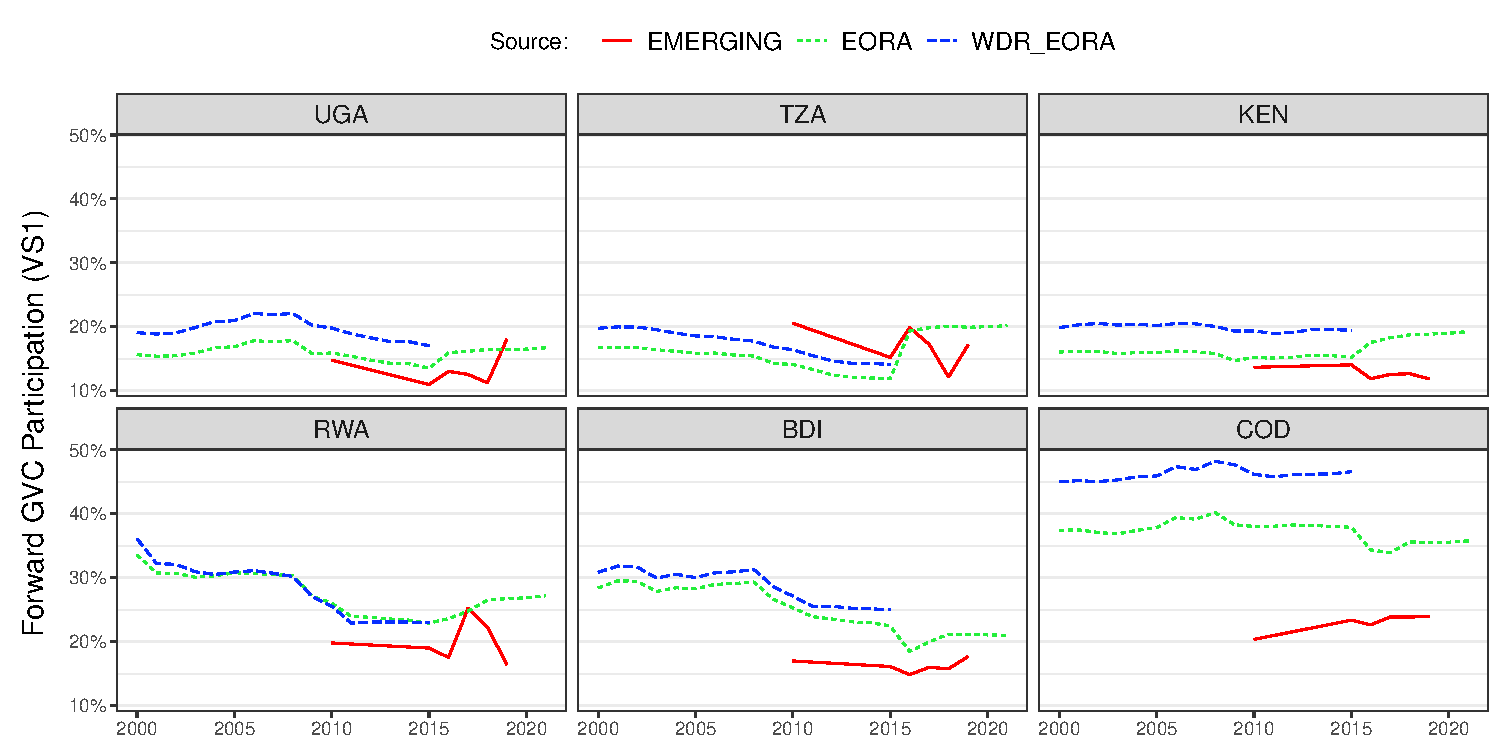
\includegraphics[width=1\textwidth]{"../Figures/REV/GVCF_shares_ag_ts.pdf"} \\ \raggedright
\scriptsize
\emph{Notes:} \citet{borin2019measuring}'s index of forward GVC integration (VS1) is the (non-double counted) DVA in exports that is not directly absorbed by the direct importer, divided by gross exports: (DVA - DAVAX)/E. 
\end{figure}
\FloatBarrier

Since even with 5-sector ICIO tables, bilateral GVC indicators using \citet{belotti2020icio}'s ICIO STATA package are extremely time-consuming, I compute the simple VS1 measure following Eq. \ref{eq:VS1} (also called exports to re-exports (E2R) by \citet{baldwin2015supply}) to examine bilateral relationships. Figure \ref{fig:EACVS1_ctry} offers a breakdown of VS1 by GVC partner. The headers indicate that E2R (Eq. \ref{eq:VS1}) is indeed upward biased vis-a-vis the corrected measure of \citet{borin2019measuring} (BM), but this does not necessitate bias in the GVC partner shares. According to EM, 4.4\% of Kenya's VS1 was re-exported by Uganda, and 3.2\% of Ugandan VS1 is re-exported by Kenya. Other EAC countries also re-export a small share of their VS1 through Kenya: Burundi (1.25\%), Rwanda (1.5\%), and Tanzania (1.5\%). Burundi and Rwanda export 2.4\% and 0.8\% of their VS1 through Uganda, respectively. Forward GVC linkages in the EAC are almost an order of magnitude smaller than backward linkages. The major GVC partner for EAC countries is the EU, accounting for 43\% of Kenyan and Congolese VS1 and close to 30\% of VS1 in the other EAC members. The early literature (e.g., \citet{foster2015global}, \citet{Kummritz20161}) associates increased VS1 with productive upgrading, which, according to Figure \ref{fig:EACVS1_ctry}, is still in its infancy in EAC RVCs. \newline

\begin{figure}[h!]
\centering
\caption{\label{fig:EACVS1_ctry}\textsc{EAC Forward GVC Participation: Re-Exporting GVC Partners}}
\small{\textit{Average EMERGING 2015-2019 Re-Exported Content Shares (VS1)}}
\vspace{2mm}
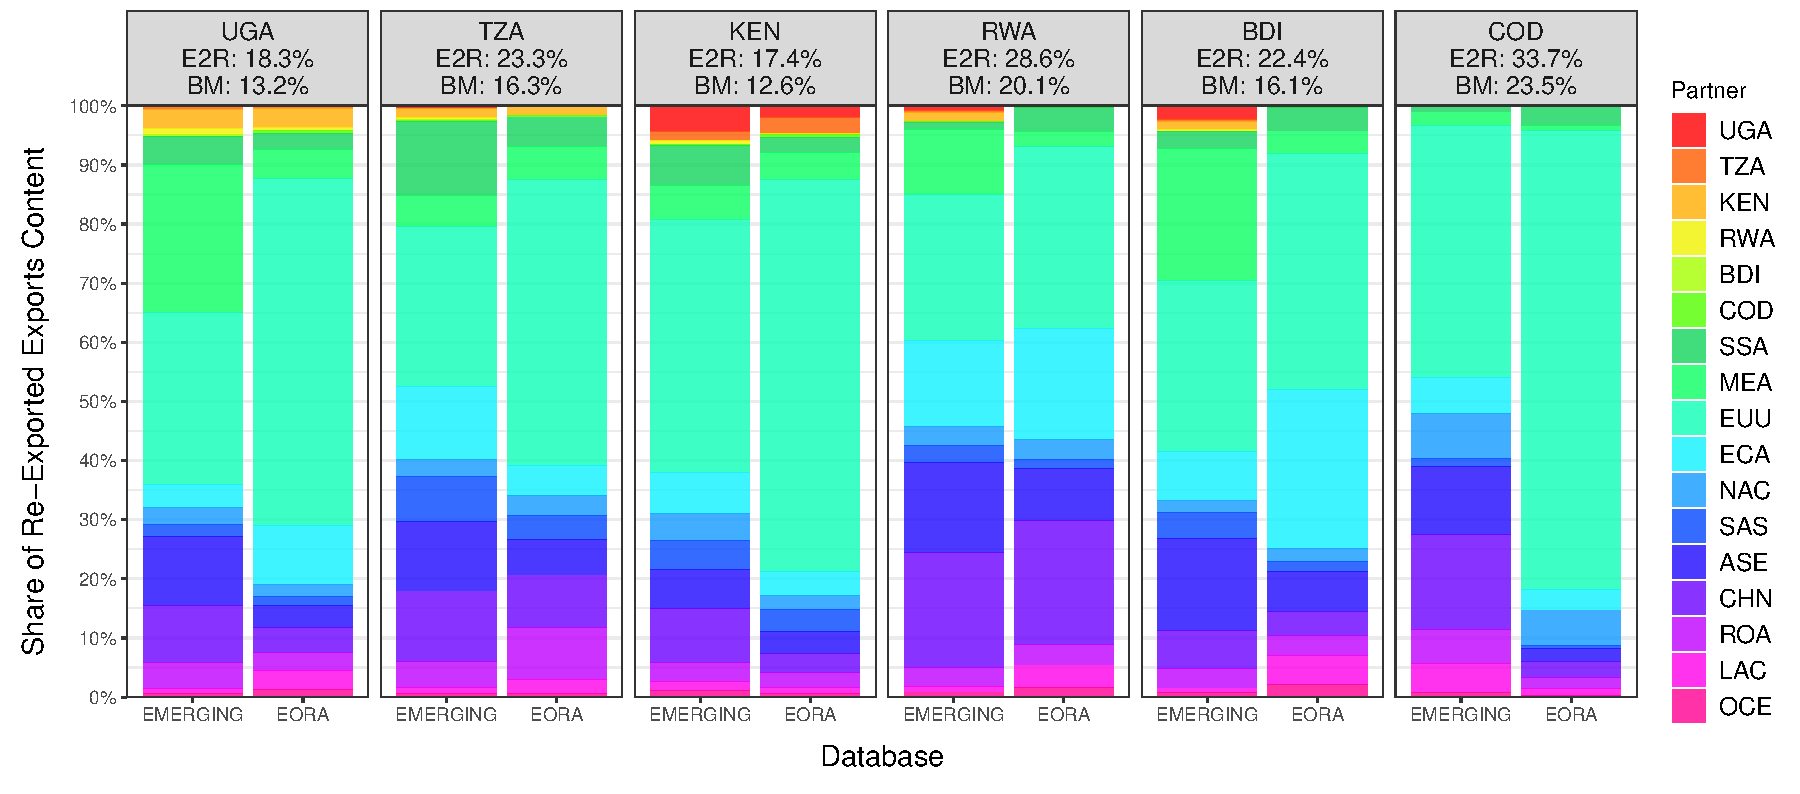
\includegraphics[width=1\textwidth]{"../Figures/REV/VS1_shares_ctry.pdf"} \\ \raggedright
\scriptsize
\vspace{-3mm}
\emph{Notes:} Figure shows a breakdown of forward GVC integration by GVC partner according to EM 2015-2019 averages. The classical VS1 measure of \citet{daudin2011produces} (Eq. \ref{eq:VS1}, also termed E2R) is used to determine each partner's share in total VS1. The headers provide overall VS1 using both E2R and the corrected measure by \citet{borin2019measuring}. 
\end{figure}
% \FloatBarrier

Table \ref{tab:EACVS1_sec} shows total forward GVC participation by sector, similar to Table \ref{tab:EACVB_sec} for backward GVC participation, and highlights considerable heterogeneity across EAC countries and sectors. In the EAC5 (excl. Congo), around 21\% of gross exports in agriculture and manufactured products are re-exported as part of GVCs. \newline

\begin{table}[h]  
\centering
\caption{\label{tab:EACVS1_sec}\textsc{EAC Forward GVC Participation: Sectoral Heterogeneity}}
\small{\textit{Average EMERGING 2015-2019 Re-Exported Content Share (\%) (VS1 following BM)}} \\
\vspace{1mm}
\begin{tabular}{lrrrrrrrrrr}
  \toprule
sector & UGA & TZA & KEN & RWA & BDI & COD & Mean & Median & EAC6 & EAC5 \\ 
  \midrule
AFF & 16.1 & 17.0 & 27.8 & 13.5 & 21.0 & 21.8 & 19.5 & 19.0 & 21.3 & 21.2\\ 
  MIN & 28.1 & 14.3 & 15.7 & 3.4 & 6.8 & 31.1 & 16.6 & 15.0 & 30.7 & 14.7\\ 
  FBE & 11.3 & 19.3 & 11.4 & 13.2 & 19.2 & 15.6 & 15.0 & 14.4 & 13.3 & 12.9\\ 
  MAN & 22.0 & 23.4 & 11.9 & 42.8 & 21.6 & 23.7 & 24.2 & 22.7 & 22.5 & 21.0\\ 
  SRV & 7.8 & 10.2 & 10.0 & 7.6 & 8.3 & 12.1 & 9.3 & 9.2 & 9.6 & 9.5\\
   \bottomrule \\ [-0.9em]
\multicolumn{11}{l}{\parbox{0.85\textwidth}{\scriptsize
\textit{Notes:} Table reports total forward GVC participation (VS1) following  \citet{borin2019measuring} using the EM 2015-2019 average in percentage terms. These shares are reported for each EAC6 country and for the EAC6 and EAC5 as a whole, which includes re-exported VA by EAC members among each other. They are thus export-weighted averages. The 'Mean' and 'Median' columns give unweighted EAC6 averages.}}
\end{tabular}
\end{table}
% \FloatBarrier

Since EAC forward GVC integration focuses on Uganda and Kenya, I also examine this link at the sector level. Based on EM 2015-19 averages, Kenya exports 81 million USD through Uganda, which amounted to 4.4\% of Kenya's VS1 and 0.76\% of its gross exports. 54\% of these 81 million are manufactured goods, 20\% are services, and 17\% are agricultural products. Uganda, on the other hand, exports 30 million USD through Kenya, which amounts to 3.2\% of Ugandan VS1 and 0.58\% of Ugandan gross exports. Of these 30 million, 45\% are agricultural products, 22\% services, 16\% FBE, and 18\% other manufacturing. The links between these two countries account for the bulk of EAC forward GVC integration, summarized compactly by Table \ref{tab:EACVS1_ctry_sec}. Of particular interest in this table is the EAC share in sectoral VS1, which is high at 20.7\% for Kenyan manufactures, indicating that about 1/5th of re-exported VA in Kenyan manufacturing is exported by its EAC partners. Other notable figures are the 41\%/29\% EAC shares in re-exported Rwandan/Kenyan mining exports, which are, however, very small in value. \newline

\begin{table}[h!] 
\centering
\caption{\label{tab:EACVS1_ctry_sec}\textsc{EAC Forward GVC Integration at the Sector Level}}
\small{\textit{Average EMERGING 2015-2019 Traditional VS1 Estimates \citep{daudin2011produces}  }} \\ \vspace{1mm}
\resizebox{\textwidth}{!}{
\begin{tabular}{lrrrrrrrrrrrrr}
  \toprule
  & \multicolumn{5}{c}{VS1 (Re-Exported By EAC Partners)} & \multicolumn{3}{c}{Total + EAC Shares} & \multicolumn{5}{c}{EAC Share in Sectoral VS1} \\
Country & AFF & FBE & MAN & MIN & SRV & SUM & VS1 & EXP & AFF & FBE & MAN & MIN & SRV \\ 
  \midrule
UGA & 18.23 & 6.05 & 13.52 & 0.00 & 11.98 & 49.78 & 5.60 & 0.95 & 6.36 & 9.05 & 6.37 & 6.79 & 4.12 \\ 
  TZA & 11.06 & 9.20 & 12.40 & 1.15 & 17.64 & 51.45 & 2.80 & 0.61 & 3.44 & 5.89 & 3.03 & 8.91 & 1.91 \\ 
  KEN & 19.58 & 9.24 & 65.88 & 0.98 & 28.33 & 124.01 & 6.83 & 1.17 & 3.22 & 6.50 & 20.74 & 28.73 & 3.86 \\ 
  RWA & 3.63 & 3.08 & 3.39 & 0.00 & 3.59 & 13.69 & 2.86 & 0.80 & 13.98 & 12.99 & 1.21 & 41.04 & 2.27 \\ 
  BDI & 0.37 & 1.27 & 0.38 & 0.01 & 0.33 & 2.37 & 4.37 & 0.97 & 5.49 & 7.49 & 2.98 & 3.01 & 2.24 \\ 
  COD & 0.22 & 0.10 & 1.33 & 0.46 & 0.34 & 2.45 & 0.06 & 0.02 & 0.07 & 0.08 & 0.06 & 0.05 & 0.07 \\ 
   \bottomrule \\ [-0.9em]
\multicolumn{14}{l}{\parbox{1.05\textwidth}{\scriptsize
\textit{Notes:} VS1 is recorded in million USD, shares in percentage terms. Column 'SUM' gives total country VS1 through EAC partners, and columns 'VS1' and 'EXP' give the share of this in the country's total VS1 and gross exports, respectively.}}  \vspace{-1mm}
\end{tabular}
}
\end{table}
% \FloatBarrier

To complete the picture, Figure \ref{fig:EACVS1_ctry_sec} shows the sector-level shares in forward GVC partners for the EAC5 (Excl. Congo). The EAC share is highest in mining at 13\%, but, Congo being excluded, mining VS1 comprises only 13 million USD, compared to 2.8/3 billion in AFF/FBE, 7.8 billion in manufacturing, and 5.6 billion in services re-exports. Among these, the EAC has a share of 4\% in AFF and 6.7\% in both FBE and MAN, indicating that manufacturing accounts for the bulk of GVC forward regional integration. The biggest forward GVC partner in all sectors remains the EU, at shares between 47\% for AFF and 16\% for MIN and MAN. 

\begin{figure}[h!] 
\centering
\caption{\label{fig:EACVS1_ctry_sec}\textsc{EAC Forward GVC Participation: GVC Partners by Sector}}
\small{\textit{Based on Average EMERGING 2015-2019 EAC Exports (Excl. Congo)}} \\
\vspace{1mm}
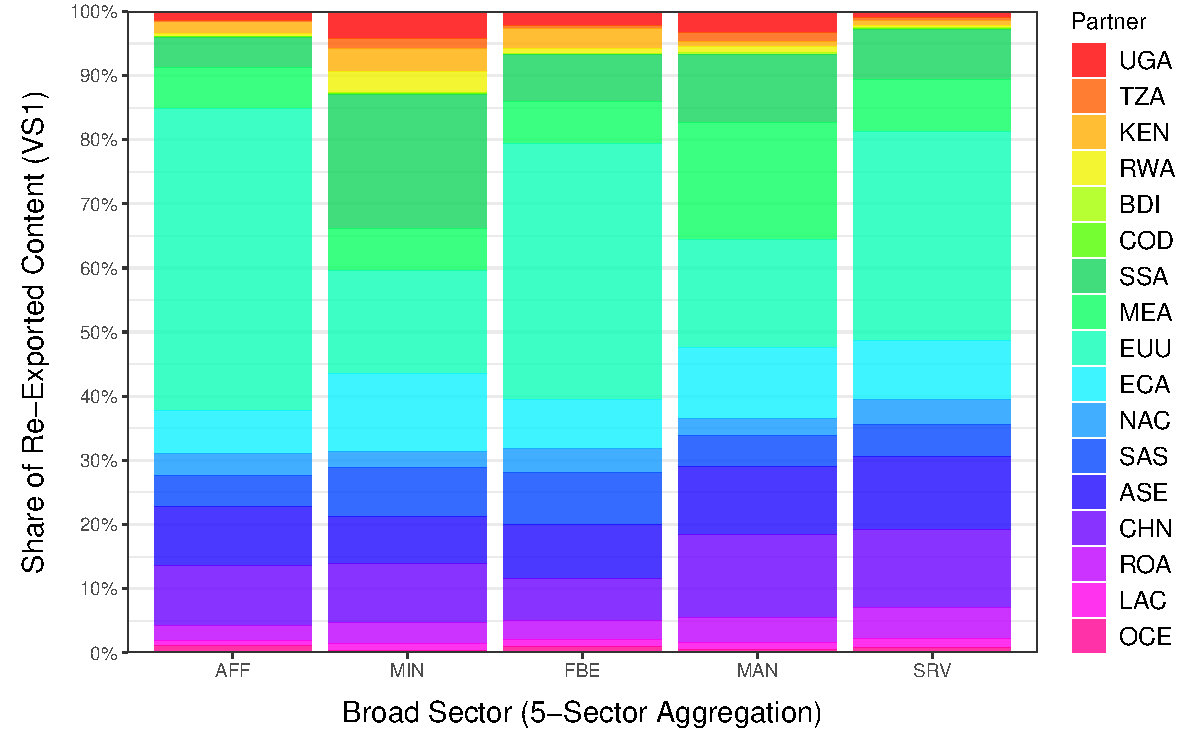
\includegraphics[width=0.7\textwidth]{"../Figures/REV/VS1_shares_sec_ctry.pdf"} \\ \raggedright
\scriptsize
\vspace{-1mm}
\emph{Notes:} Figure shows a sector-level breakdown of total EAC5 VS1 (E2R) by GVC partner using EM (2015-2019) averages. % \\ \vspace{-5mm}
\end{figure}
\FloatBarrier



\subsection{Trends in EAC Regional Integration in Value Added Terms}

While overall EAC GVC integration appears relatively stable, exempting an increase in VS in the smaller economies and a gradual decline in VS1, there may be stronger trends in regional integration relative to overall trade and GVC integration - as evident in gross trade flows. In this section, I thus introduce four metrics to track EAC regional integration through VA in supply chains relative to the members' overall GVC participation. The first metric is the share of FVA in a member's production/exports accounted for by its EAC neighbours. It is defined as 
%
\begin{equation} \label{eq:VS_EAC}
\text{VS}_{uj}^\text{EAC} = \frac{1}{\text{VS}_{uj}}  \sum_{oi \in \text{EAC},\ o \neq  u} \text{vb}_{oi, uj}   \ \ \forall\ uj \in \text{EAC},
\end{equation} 
%
\noindent where VS$_{uj}$ is defined as in Eq. \ref{eq:VS}. VS$^\text{EAC}$ is thus a relative measure tracking the EAC share in VS, as shown also in Figure \ref{fig:EACVB_ctry}, such that the overall EAC VA share in domestic production/exports can be computed as VS$_{uj}^\text{EAC} \times \text{VS}_{uj} \ \forall\ uj$. I define an analogous measure for VS1 as the proportion of DVA in re-exported exports exported by EAC partner states, also visible in Figure \ref{fig:EACVS1_ctry}
%
\begin{equation} \label{eq:VS1_EAC}
\text{VS1}_{oi}^\text{EAC} =  \sum_{uj \in \text{EAC}, u \neq  o} \text{vbe}_{oi, uj} \bigg/ \sum_{uj, u \neq  o} \text{vbe}_{oi, uj}\ \ \forall\ oi \in \text{EAC}.
\end{equation}
%
These two metrics effectively track the role of the EAC in members' GVC participation. They, however, do not account for the import side, i.e., the EAC's role in providing goods and services to members' relative to ROW. I thus compute two additional metrics to capture this aspect of regional integration. The first is the share of EAC VA in members' imports, which I denote by VAI$^\text{EAC}$. Consider $\textbf{e}_u$ the vector of gross exports to EAC using country $u \in \text{EAC}$ from each country-sector. I then compute the VA origins of these exports to country $u$ as 
%
\begin{equation}
\textbf{e}_u^\text{VA} = \textbf{VBe}_u,
\end{equation}
%
\noindent where $\textbf{e}_u^\text{VA}$ denotes the vector, with elements $e_{oi, u}^\text{VA}$, of VA supplied by each country-sector ($oi$) in these imports of country $u$. From  $\textbf{e}_u^\text{VA}$, the share of EAC VA is easily computed as 
%
\begin{equation}
\text{VAI}_u^\text{EAC} = \sum_{oi \in \text{EAC}, o \neq u}  e_{oi, u}^\text{VA}  \bigg/ \sum_{oi, o \neq u}  e_{oi, u}^\text{VA}.  
\end{equation}
%
VAI$_u^\text{EAC}$ is thus a country-level measure of EAC VA in the import mix. It may include intermediates of goods being exported. To single out the EAC share in imported consumption goods, I also consider only exports for final consumption. Let $\textbf{fe}_u$ be the final exports to country $u$ from each country-sector. Then $\textbf{fe}_u^\text{VA} = \textbf{VBfe}_u$ denotes these exports in VA terms, and I define
%
\begin{equation} \label{eq:VAFI_EAC}
\text{VAFI}_{u}^\text{EAC} = \sum_{oi \in \text{EAC}, o \neq u}  \textbf{fe}_{oi, u}^\text{VA}  \bigg/ \sum_{oi, o \neq u}  \textbf{fe}_{oi, u}^\text{VA}
\end{equation}
%
\noindent as the EAC VA share in final goods exported to a particular member $u$. I compute these metrics using the MRIO tables with reduced country dimension, except for $\text{VS1}_{oi}^\text{EAC}$, where I use the tables with reduced sectoral dimension. Figure \ref{fig:VAEACshares} plots all metrics, including a weighted linear trend.\footnote{All observations receive a weight of 1, except for EM 2010 obs. which receive a weight of 2 because no further data is observed until 2015, and EORA 2016-21 obs. receive a weight of 0.1 due to the stark structural break. \vspace{-4mm}}

\begin{figure}[h!] 
\centering
\caption{\label{fig:VAEACshares}\textsc{EAC5 VA Shares in Members VS, VS1, Imports and Final Imports}}
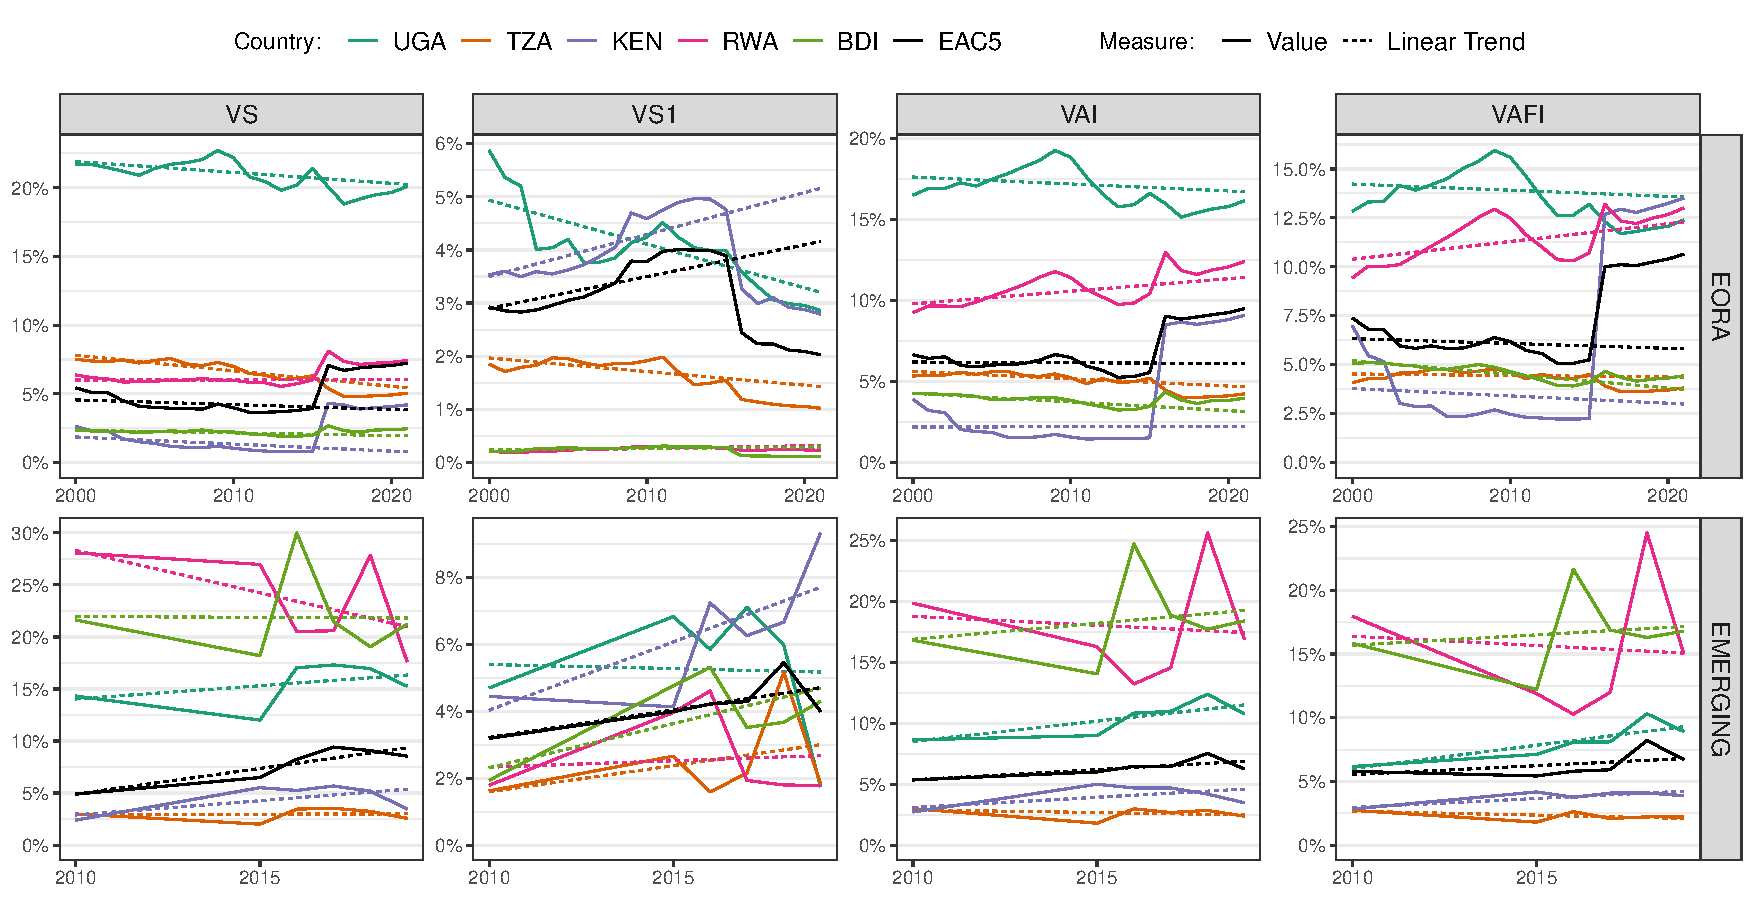
\includegraphics[width=1\textwidth, trim= {0 0 0 0}, clip]{"../Figures/REV/VA_EAC5_shares_ts.pdf"} \\ 
\raggedright
\scriptsize
\emph{Notes:} Figure shows regional EAC regional integration metrics following Eqns. \ref{eq:VS_EAC}-\ref{eq:VAFI_EAC}, including a (weighted) linear trend. 
\end{figure}
\FloatBarrier

Both databases agree that EAC shares in members' VS1 are substantially lower than in VS, VAI, and VAFI but increased over the period, mainly driven by Kenya. They also agree that the larger economies drive EAC forward linkages, and smaller economies (Rwanda and Burundi) are more important in backward linkages (VS) and as importers of final goods (VAFI). Otherwise, there is not much agreement regarding the direction of the trend. Figure \ref{fig:VAEACshares_bar} plots the slope coefficients.


\begin{figure}[h!] \vspace{-1mm}
\centering
\caption{\label{fig:VAEACshares_bar}\textsc{Weighted Slope Estimates Measuring the Speed of Regional Integration}}
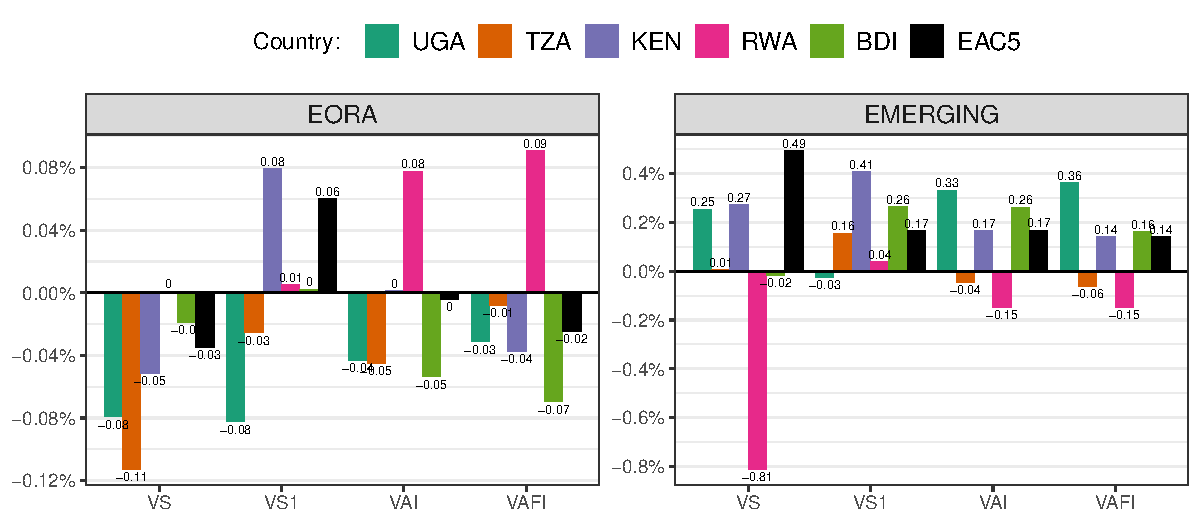
\includegraphics[width=1\textwidth, trim= {0 0 0 0}, clip]{"../Figures/REV/VA_EAC5_shares_slope_bar.pdf"} \\ 
\raggedright
\scriptsize
\emph{Notes:} Figure shows (weighted) linear slopes (dotted lines in Figure \ref{fig:VAEACshares}). In the estimation, all obs. received a weight of $w=1$, except for EM 2010 ($w=2$) and EORA $>$ 2015 ($w=0.1$). These weights reflect data availability and quality.  
 \vspace{-4mm}
\end{figure}
\FloatBarrier

 The more reliable EM database suggests that, with few exceptions, EAC regional integration in VA terms is increasing in most countries. Considering the EAC5 as a whole, the coefficients suggest that $\text{VS}^\text{EAC}$ is increasing by 0.5 percentage points (pp.) per year, and the EAC shares in EAC VS1, VAI, and VAFI are increasing at a slower rate of around 0.15 pp. per year. These trends mildly contrast those in gross trade (Figure \ref{fig:GTEACshares}). \newline

As with gross trade, the weak aggregate signal indicates that there may be more substantial sectoral developments. I thus recompute all 4 indicators at the sector level using the EM database with full country dimension but only 5 broad sectors. Figure \ref{fig:VAEACshares_bar_sec} shows weighted linear slope estimates at the sector level (excluding mining), using again a weight of $2$ for 2010 estimates. 

\begin{figure}[h!] 
\centering
\caption{\label{fig:VAEACshares_bar_sec}\textsc{Weighted Slope Estimates of Members Sectoral Integration Speed}}
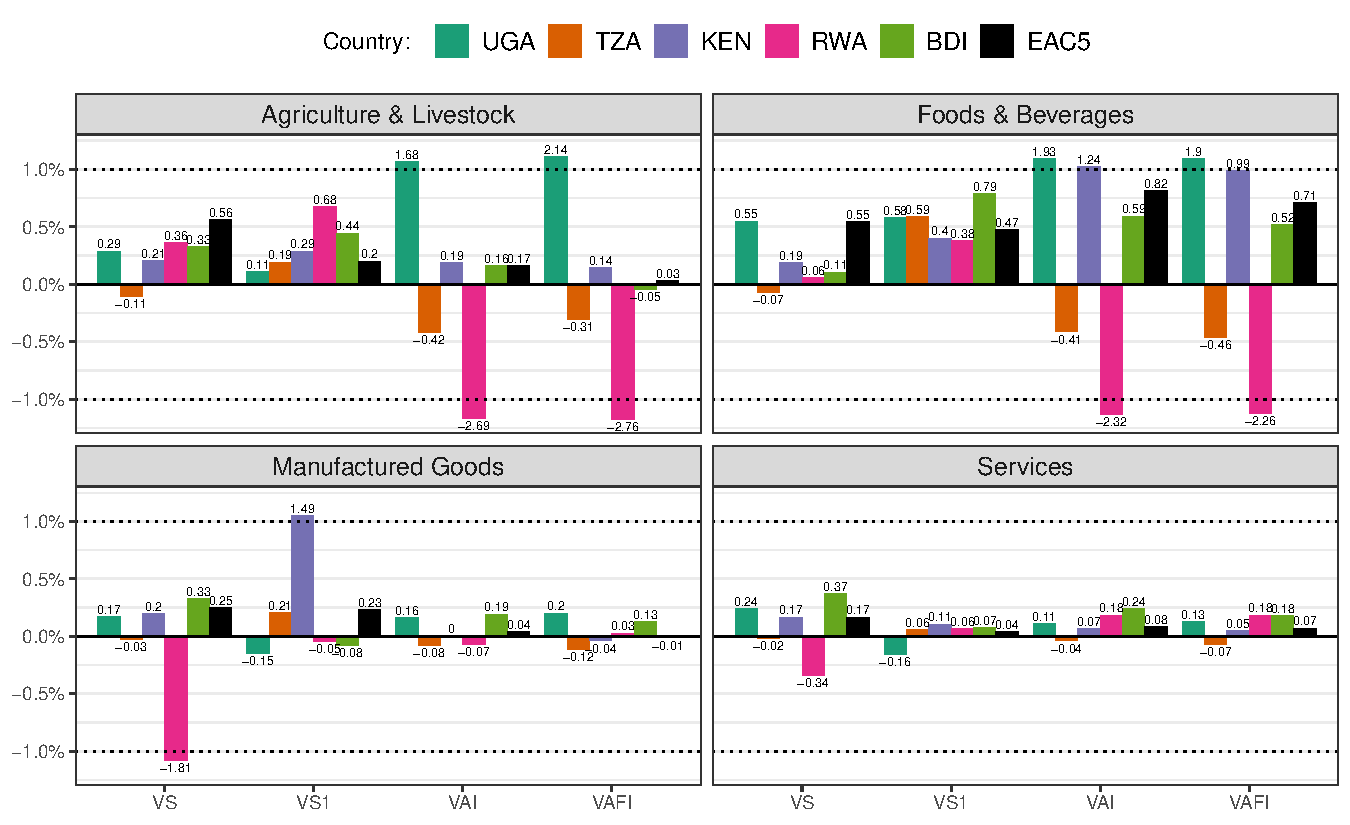
\includegraphics[width=1\textwidth, trim= {0 0 0 0}, clip]{"../Figures/REV/EM_VA_EAC5_shares_slope_bar_sec.pdf"} \\ \raggedright
\scriptsize
\emph{Notes:} Figure shows (weighted) linear slopes estimating the speed of regional integration (pp. per year) at the 5-sector level (excl. mining) based on EM (2010-2019). All obs. received a weight of $w=1$, except for EM 2010 ($w=2$).  
\end{figure}
\FloatBarrier

Regional integration in goods-producing sectors proceeds substantially faster than in services. The aggregate pattern from Figure \ref{fig:VAEACshares_bar}, with faster integration through $\text{VS}^\text{EAC}$, is reflected in agriculture, manufacturing, and services. The FBE sector, on the other hand, experienced stronger integration through forward linkages ($\text{VS1}^\text{EAC}$) and imports ($\text{VAI}^\text{EAC}$, $\text{VAFI}^\text{EAC}$) at greater speeds ($\geq 0.5$ pp. per year on all metrics). Uganda and Kenya are driving these developments. The regional integration in FBE through $\text{VS1}^\text{EAC}$ is driven by all 5 members at almost equal shares, whereas the manufacturing expansion through $\text{VS1}^\text{EAC}$, proceeding at about half the speed as FBE, is driven almost completely by Kenya, with Tanzania contributing a little bit, and other members experiencing declining $\text{VS1}^\text{EAC}$. This analysis of regional integration in VA terms thus complements Figures \ref{fig:EAC_ROW_Ratios_Sec} and \ref{fig:GTEACsharesSec}, indicating that there is some momentum in regional integration through agriculture and FBE, but equitable integration in manufacturing is difficult, and Kenya is strengthening its already favourable trading position through forward GVC linkages. 


\subsection{EAC Positioning in GVCs}

Following \citet{antras2012measuring, antras2022global}, a common measure of upstreamness $U_{oi} \ \in \ $ \textbf{u} is obtained by iterating forward the IO model in Eq. \ref{eq:io_model}, multiplying terms by the number of production stages needed to obtain them, and normalizing by gross output. In matrix notation: 
%
\begin{equation} \label{eq:upstreamness}
\textbf{u}\textbf{x} = \textbf{d} + 2\textbf{Ad} + 3\textbf{AAd} + 4\textbf{AAAd} + \cdots = (\textbf{I}-\textbf{A})^{-2}\textbf{d}.
\end{equation}
%
The index is, by definition, greater than 1, and \citet{antras2012measuring} state that it can be interpreted as the dollar amount by which the output of all country-sectors combined increases following a one-dollar increase in the VA of sector $i$ in country $o$. Intuitively, it measures the distance of the production stage performed by sector $i$ in country $o$ to the finally demanded product (\textbf{d}).\footnote{\label{fn:ds} An equivalent measure of downstreamness (\textbf{d}) can be computed measuring the distance to VA instead of FD \citep{antras2022global, miller2017output, mancini2023positioning}, but, for the sake of brevity, this is omitted. The simplest way of computing this index is as $\textbf{d}=\textbf{1}'\textbf{B}$, i.e., it is the column-sum of the Leontief inverse matrix \citep{miller2017output, antras2022global}. It can be interpreted as the total increase in gross output in the world economy that a unit increase in FD in the respective country-sector would generate. At the world level \textbf{u} and \textbf{d} are identical and measure the length of GVCs \citep{mancini2023positioning}.} \citet{antras2012measuring} further find that $U$ is positively correlated with physical capital intensity and negatively correlated with skill intensity across US industries, and negatively correlated with rule of law, private credit to GDP, and education across a sample of OECD countries. Figure \ref{fig:EACUS_ag_ts} shows aggregate upstreamness for the EAC, calculated using the regional MRIO tables with the full sector dimension, where sector-level $U_{oi}$ estimates were averaged using gross export weights. 

\begin{figure}[h!]
\centering
\caption{\label{fig:EACUS_ag_ts}\textsc{Upstreamness Index for EAC Countries}}
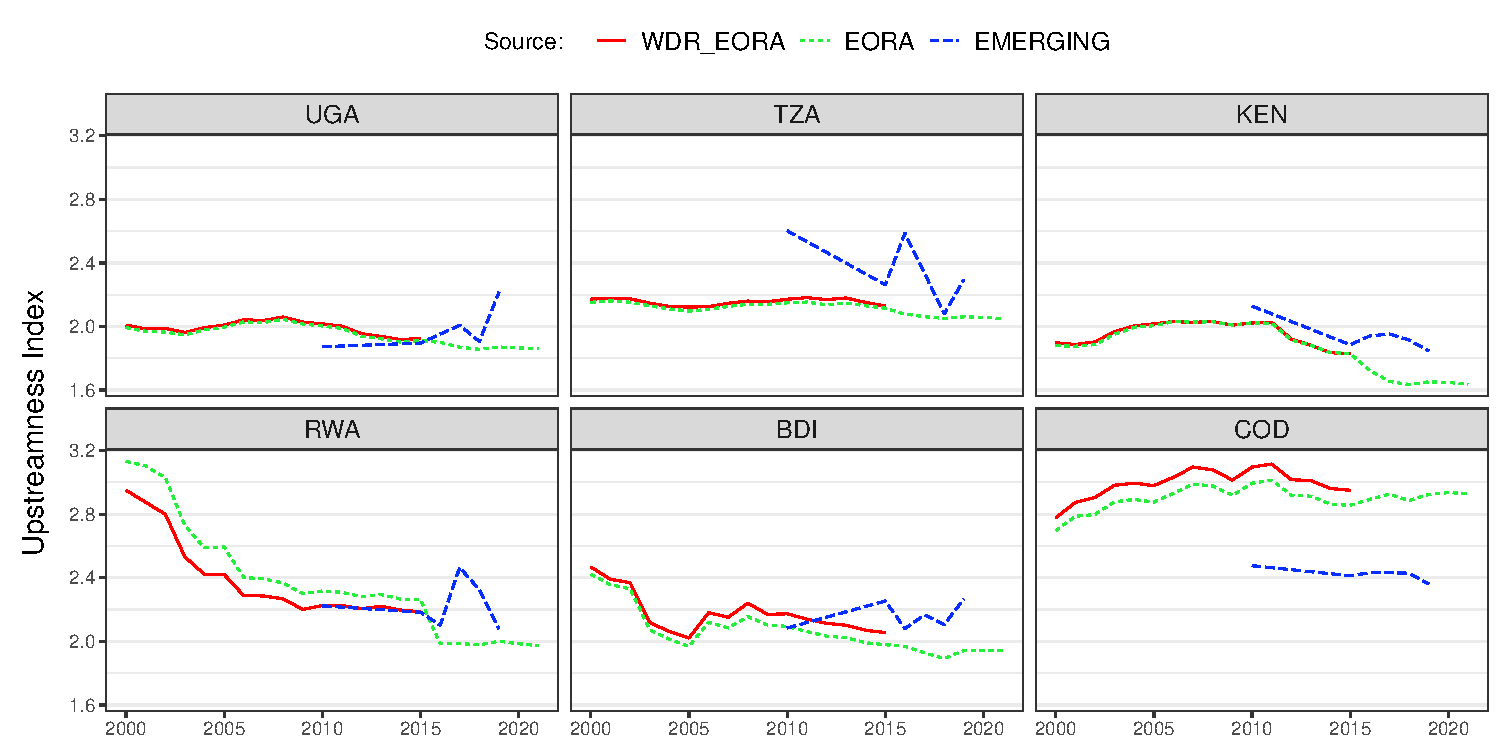
\includegraphics[width=1\textwidth]{"../Figures/REV/Upstreamness_ag_ts.pdf"} \\ \raggedright
\scriptsize
\emph{Notes:} Figure shows upstreamness index following \citet{antras2012measuring}, computed at the sector level and averaged across sectors using sectoral gross exports as weights. The EORA and EM MRIOs have EAC + 11 regions and all sectors.  
\end{figure}
\FloatBarrier

Figure \ref{fig:EACUS_ag_ts} shows that the computed $U$ index closely tracks the version computed by \citet{mancini2023positioning} using the full EORA 26 database and also performing an inventories adjustment following \citet{antras2018measurement}. The data suggest that Congo, as a large commodity exporter, is very upstream, while other members apart from Uganda and Burundi, where EM suggests a slight increase, have moved more downstream since 2010. Rwanda also shows an impressive downstream shift in 2000-2010, but this trend must be scrutinized as EORA lacks a Rwandan IO table. \newline

To investigate developments at the sector level, I aggregate $U$ to broad sectors using export weights, combining all manufacturing sectors apart from FBE and all service sectors into broad categories. I also aggregate the time dimension over two intervals, 2010-2014 and 2015-2019, using the median to obtain a robust estimate. Table \ref{tab:U_BSEC} reports the results, including an estimate of the growth rate of $U$ between the two intervals and an export-weighted EAC5 average. \newline 

 The most upstream sector, according to both databases, is MIN, where $U>3$ implies more than 3 production stages on average before final use. This is followed by MAN with $2 <U <3$ in most members, FBE and primary AFF with $1.5 <U <2.5$, and SRV with $1 <U <2$. Except for SRV, this is broadly in line with the world average sectoral upstreamness pattern of, according to EM 2015-19, 3.32 (MIN), 2.86 (MAN), 2.62 (AFF), 2.25 (SRV) and 2.18 (FBE). The $U$ values of around 2/2.5 for EAC FBE/MAN indicate that these sectors are located at least one step before final use. For FBE, where more than 90\% of VS1 is through non-EAC GVC partners (Figure \ref{fig:EACVS1_ctry_sec}), this implies that more processing steps could still be undertaken regionally to export products closer to FD. The change between the two intervals indicates a downstream shift in almost all country-sectors. It is particularly pronounced in AFF, MAN, and FBE, but also in SRV. The shift suggests that all production processes are moving closer to FD. The world average growth rate in $U$ between these intervals, according to EM, was 3.3\% for AFF, 2.1\% for MIN, 0.85/0.82\% for FBE/MAN, and -0.5\% for SRV, revealing that, except for SRV, EAC developments run against a global trend towards longer manufacturing GVCs \citep{antras2018measurement}. 

\begin{table}[h!] 
\centering
\caption{\label{tab:U_BSEC} EAC5 Trends in Upstreamness by Broad Sector (Aggregated)}
\vspace{2mm}
\resizebox{\textwidth}{!}{
\begin{tabular}{llrrrrrrrrrrrr}
  \toprule
  && \multicolumn{6}{c}{WDR Estimates using EORA 2015} & \multicolumn{6}{c}{EMERGING Estimates} \\
\\Sector & Year & UGA & TZA & KEN & RWA & BDI & EAC5 & UGA & TZA & KEN & RWA & BDI & EAC5 \\ 
  \midrule
  AFF & 2010-2014 & 2.17 & 2.38 & 1.56 & 2.36 & 3.49 & 1.81 & 1.86 & 1.88 & 2.30 & 1.80 & 1.98 & 2.09 \\ 
  AFF & 2015-2019 & 2.13 & 2.36 & 1.49 & 2.35 & 3.33 & 1.76 & 1.91 & 1.84 & 1.83 & 1.28 & 1.77 & 1.84 \\ 
  AFF & Growth Rate & -1.72 & -0.94 & -4.11 & -0.49 & -4.75 & -2.68 & 2.85 & -2.08 & -20.64 & -29.25 & -10.73 & -12.06 \\ 
  MIN & 2010-2014 & 3.07 & 3.53 & 3.49 & 3.39 & 2.89 & 3.48 & 2.13 & 3.23 & 3.28 & 3.29 &  & 3.25 \\ 
  MIN & 2015-2019 & 3.02 & 3.37 & 3.45 & 3.32 & 2.81 & 3.41 & 3.22 & 3.28 & 3.12 & 1.54 & 1.63 & 3.17 \\ 
  MIN & Growth Rate & -1.62 & -4.46 & -1.40 & -2.23 & -2.81 & -2.08 & 51.20 & 1.56 & -5.02 & -53.27 &  & -2.44 \\ 
  FBE & 2010-2014 & 1.47 & 1.58 & 1.41 & 1.39 & 1.50 & 1.45 & 2.23 & 2.04 & 2.34 & 2.57 & 2.32 & 2.26 \\ 
  FBE & 2015-2019 & 1.44 & 1.57 & 1.34 & 1.36 & 1.45 & 1.38 & 2.15 & 2.12 & 2.18 & 2.35 & 2.41 & 2.13 \\ 
  FBE & Growth Rate & -2.26 & -0.88 & -5.32 & -1.87 & -2.81 & -4.37 & -3.21 & 3.81 & -6.57 & -8.54 & 4.25 & -5.59 \\ 
  MAN & 2010-2014 & 2.20 & 2.09 & 2.30 & 2.19 & 2.03 & 2.25 & 2.38 & 3.28 & 2.41 & 3.84 & 3.17 & 2.89 \\ 
  MAN & 2015-2019 & 2.14 & 2.06 & 2.18 & 2.15 & 1.97 & 2.15 & 2.47 & 2.89 & 2.24 & 3.16 & 2.73 & 2.63 \\ 
  MAN & Growth Rate & -2.62 & -1.57 & -5.34 & -1.68 & -3.15 & -4.42 & 3.81 & -11.79 & -7.11 & -17.74 & -13.96 & -9.02 \\ 
  SRV & 2010-2014 & 1.73 & 1.89 & 1.77 & 1.70 & 1.79 & 1.78 & 1.35 & 2.19 & 1.83 & 1.40 & 1.47 & 1.82 \\ 
  SRV & 2015-2019 & 1.70 & 1.85 & 1.64 & 1.67 & 1.74 & 1.69 & 1.52 & 2.09 & 1.65 & 1.61 & 1.41 & 1.77 \\ 
  SRV & Growth Rate & -1.40 & -1.89 & -7.02 & -1.78 & -2.85 & -4.82 & 12.27 & -4.84 & -9.75 & 15.11 & -4.01 & -2.66 \\ 
   \bottomrule \\ [-0.9em]
\multicolumn{14}{l}{\parbox{1.24\textwidth}{\scriptsize
\textit{Notes:} Table shows median upstreamness ($U$) following \citet{antras2012measuring} across 2010-14 and 2015-19, and the growth rate in percentage terms between these medians. MAN and SRV are broad categories combining sectors TEX-MAN and EGW-PAO in Table \ref{tab:sec}, respectively, via an export-weighted average. The EAC5 is an export-weighted average across the 5 countries (excl. COD) computed annually before taking the median.  }}
\end{tabular}
}
\end{table}
\FloatBarrier

This appears to be good news for all sectors apart from MAN and SRV, indicating that exports are closer to FD and more local value is added. For MAN, it suggests a shift towards processing trade, which is generally not associated with industrial upgrading. The effect of SRV moving downstream is more ambiguous and depends very much on the type of service.\footnote{For transport/tourism (TRA), a downstream shift could indicate more local value addition, whereas for telecommunications (PTE) and financial intermediation (FIB), downstream shifts might signify the insufficient quality of these services to be used as intermediates in more complicated production processes. EAC data on these sectors are likely of questionable quality, yet a brief disaggregated appraisal using EM yields, notably, 28\% upstream/downstream shifts in FIB in Rwanda/Tanzania (EAC5 average is 5.3\% downstream), a 9.5/5.9\% downstream shift in PTE in Kenya/Rwanda (EAC5 average is 3\% downstream) and a 10.2/7.4\% downstream shift in TRA in Kenya/Burundi, while other members saw a slight upstream shift (EAC5 average is 1.4\% downstream). }


\section{(New) Revealed Comparative Advantage}

In international trade, including GVC-related trade, competitiveness is closely related to the concept of comparative advantage\footnote{A widely accepted theory of international trade developed by David Ricardo in 1817 stipulating that countries specialize in sectors where their productivity relative to the international average is greatest.}. 
A popular way to quantify Ricardo's concept of comparative advantage is \citet{balassa1965trade}'s measure of revealed comparative advantage, defined as the share of a sector in gross country exports divided by the share of that sector in gross world exports
%
\begin{equation}
\text{RCA}_{oi} = \frac{E_{oi}}{\sum_i E_{oi}} \Bigg/ \frac{\sum_j E_{ji}}{\sum_{ji} E_{ji}}.
\end{equation}
%
$\text{RCA}_{oi}>1$ signifies a revealed comparative advantage of country $o$ in sector $i$. The traditional index based on gross exports, however, does not account for GVCs and double counting in exports. \citet{koopman2014tracing}, therefore, propose a new index based on the DVA in gross exports. \citet{borin2019measuring} show that the decomposition of \citet{koopman2014tracing} is inexact in allocating DVA and foreign double-counted items and propose refinements. Appendix Figure \ref{fig:KWW} shows the refined breakdown following \citet{borin2019measuring}, and Appendix Figure \ref{fig:KWW_fill_ts} plots the decomposition of gross exports for each of the EAC members.\footnote{To connect this to the aggregate measures of GVC integration VS and VS1 discussed so far: VS is (DVA $-$ GX)/GX, or (DDC $+$ FVA $+$ FDC)/GX, VS1 is (DVA $-$ DAVAX)/GX or (NDAVAX $+$ REF)/GX. \vspace{-5mm}} DVA is the sum of DAVAX, NDAVAX, and REF. According to EM 2015-19, in the average EAC member, DAVAX accounts for 71\% of gross exports, NDAVAX for 12\%, FVA for 14\%, and FDC for 3\%. REF and DDC are close to 0 in all EAC countries, implying that the GVCs these countries engage in are relatively short. DVA $=$ E $-$ (DDC $+$ FVA $+$ FDC), yielding an average 17\% downward adjustment of gross exports. This may appear small, but, as Table \ref{tab:EACVB_sec} shows, manufacturing sectors have higher VS of up to 50\%. \newline
 
For comparison, I compute both classical RCA using gross exports (GX) and NRCA using DVA in exports (VAX) based on all available databases, including BACI (only available for goods-producing sectors) and the WDR GVC indicators based on EORA 2015. Figure \ref{fig:NRCA} shows median (N)RCA estimates across years 2010-19 for the EAC5. Appendix Tables \ref{tab:NRCA} and \ref{tab:NRCA_corr} contain the corresponding values and correlations among different estimates, respectively. Whereas EORA-based estimates correlate around 0.57 with the BACI estimates, EM estimates have a strong correlation of 0.93, confirming that these IO tables are very close to official trade data. In all IO tables, RCA and NRCA estimates are also highly correlated ($r > 0.96$), suggesting that the foreign content shares in exported goods within a sector are quite similar across different countries.

\begin{figure}[h!] 
\centering
\caption{\label{fig:NRCA}\textsc{(New) Revealed Comparative Advantage: 2010-19 Median}}
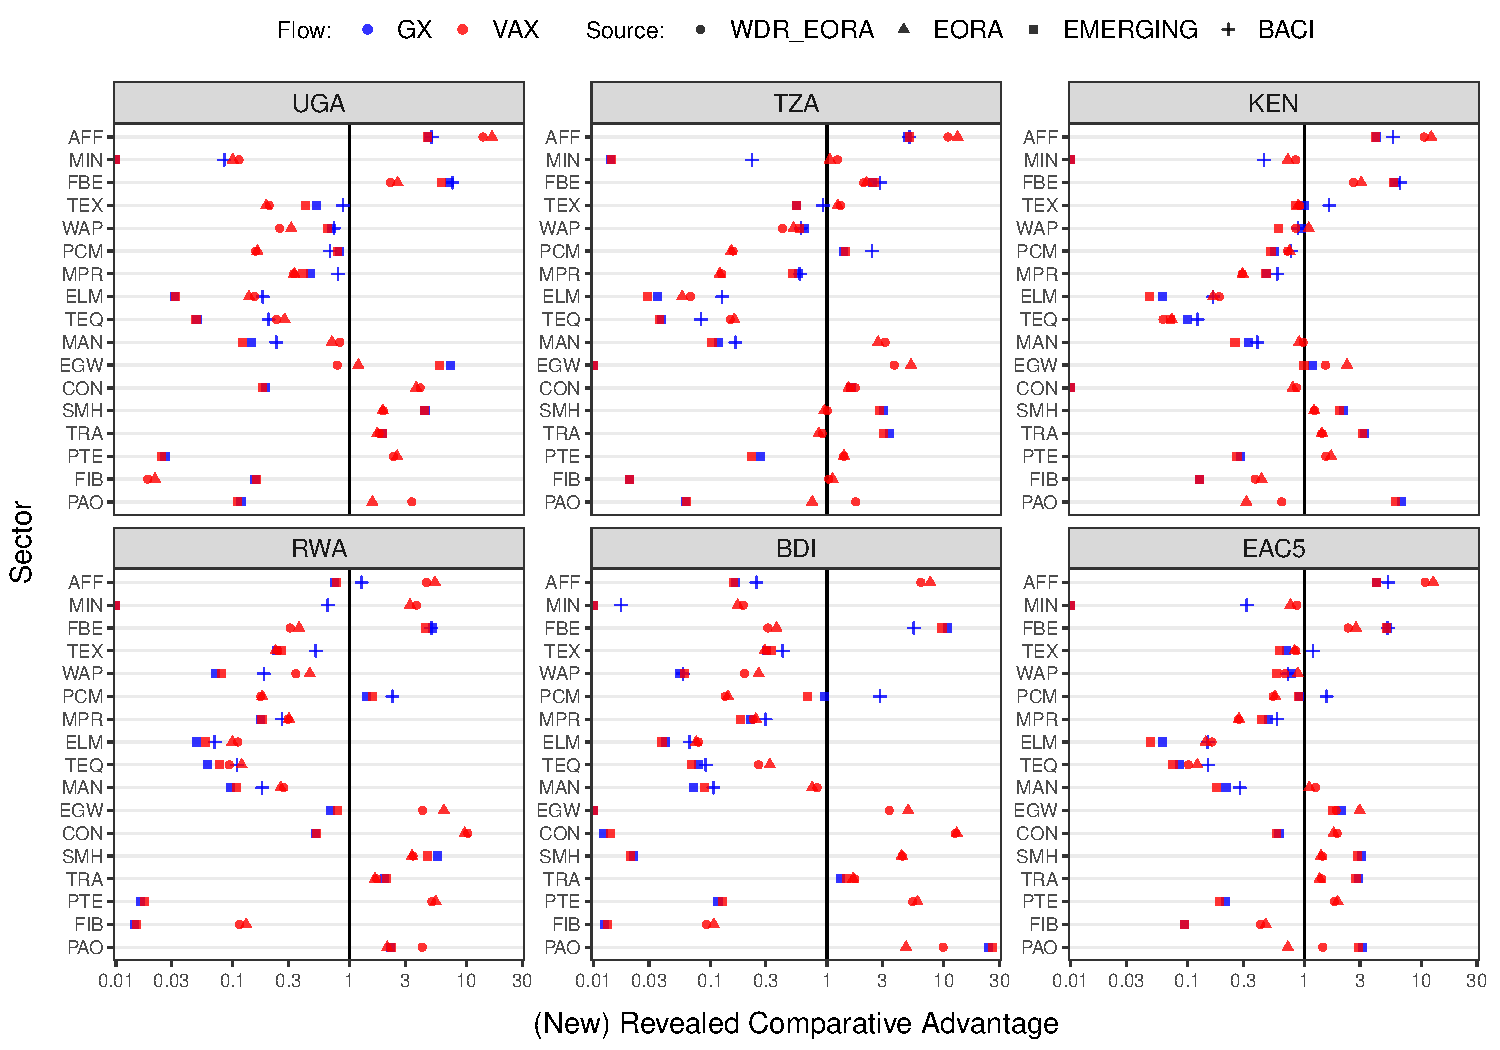
\includegraphics[width=1\textwidth]{"../Figures/REV/NRCA_EAC5_ALL.pdf"} \\
\raggedright
\scriptsize
\emph{Notes:} Figure shows median 2010-19 (N)RCA indices based on DVA/gross exports according to different databases. DVA is computed following \citet{borin2019measuring}. Appendix Table \ref{tab:NRCA} contains the values and Table \ref{tab:NRCA_corr} their correlations. To not overcrowd the figure, GX-based estimates using (WDR\_)EORA are not shown. 
\end{figure}
\FloatBarrier

All estimates show that the EAC5 as a whole, and, according to EM/BACI, also all the 5 countries individually, have a succinct (N)RCA in agriculture and food processing of, according to the EM NCRA estimates, 4.17 (AFF) and 5.01 (FBE). Similarly, all countries have a sizeable disadvantage in all core manufacturing sectors except for textiles and petrochemicals. Especially ELM (0.05) and TEQ (0.08), core drivers of GVC expansion according to the WDR, have a strong revealed disadvantage. On the services side, all members have a (N)RCA in TRA (2.77, incl. tourism), particularly Kenya (3.12) and Tanzania (3.02), and all members apart from Burundi have a (N)RCA in SMH (2.84), particularly Uganda (4.36) and Rwanda (4.64). Furthermore, with its powerful dams, Uganda has a large (N)RCA in EGW (5.87). EAC members thus exhibit similar patterns of (N)RCA in agriculture, food processing, and tourism, and a disadvantage in core manufacturing sectors. This is constitutive to forming a common trade block, supported by a monetary union as planned, and deepening regional tourism and food processing value chains. Yet, comparing the EAC with ROW masks rivalries and differences in (N)RCA between members. 



\subsection{NRCA Relative to the EAC and in Inner-EAC Trade}

To uncover these differences, I compute (N)RCA relative to the EAC5 as the share of a sector in country exports to its share in EAC5 exports. Furthermore, regional trading reveals comparative advantages that can foster or block deeper RVCs. Thus, I also compute (N)RCA w.r.t. intraregional exports. Figure \ref{fig:EAC_NRCA} presents both estimates and Appendix Table \ref{tab:EAC_NRCA} the corresponding values. 

\begin{figure}[h!]
\centering
\caption{\label{fig:EAC_NRCA}\textsc{NRCA Relative to EAC5}}
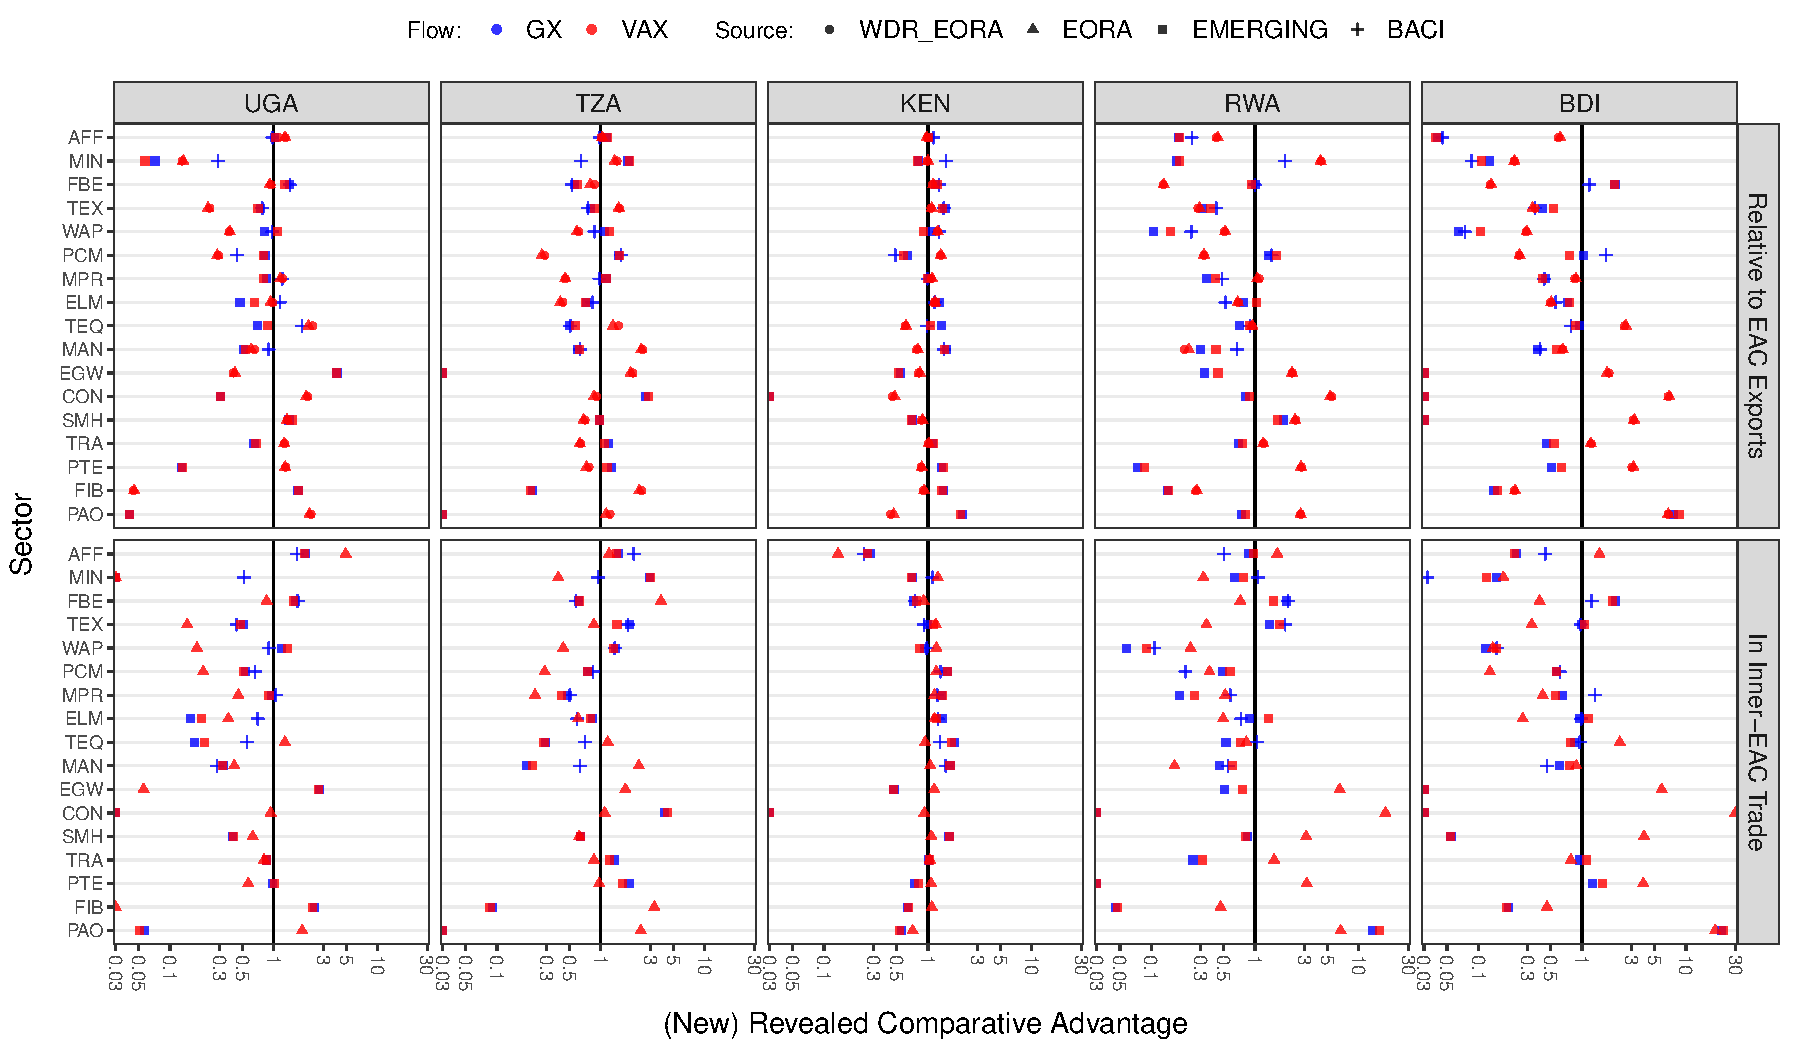
\includegraphics[width=1\textwidth]{"../Figures/REV/EAC_NRCA_EAC5_ALL.pdf"} \\
\raggedright
\scriptsize
\emph{Notes:} Figure shows median 2010-19 (N)RCA indices based on DVA/gross exports according to different databases, calculated w.r.t. EAC5 exports (top panel) and w.r.t. total inner EAC5 trade (bottom panel). DVA is computed following \citet{borin2019measuring}. Appendix Table \ref{tab:EAC_NRCA} contains the corresponding values. To not overcrowd the figure, GX-based estimates using (WDR\_)EORA are not shown.
\end{figure}
\FloatBarrier

The estimates unveil that relative to other EAC5 members, Uganda, Tanzania, and Kenya have a slight (1-1.2) (N)RCA in agriculture, and Uganda, Kenya, and Burundi have a (N)RCA in FBE of (1.2-1.5). In inner-EAC trade, Kenya's (N)RCA drops to 0.26/0.78 in AFF/FBE in VAX terms, whereas Uganda's rises to 2/1.5, reflecting its stronger regional supplier role. Rwanda has a (N)RCA in mining, but this is not reflected in inner-EAC5 trade. Kenya has a slight comparative advantage in manufacturing sectors, including TEX, MPR, ELM, TEQ, and other manufactures (MAN). Exempting TEX, including PCM, these estimates are even higher in inner-EAC5 trade, but all are in the range between 1 and 2 and thus significantly lower than with ROW. Tanzania also has a (N)RCA in PCM according to both denominations. As mentioned earlier, Kenya and, to a lesser extent, Tanzania also have a slight (N)RCA in TRA (1-1.2), both relative to the EAC and revealed in inner-EAC trade, and Uganda has a large (N)RCA in EGW (4-5). \newline

The trading patterns of different members in both gross and VA terms thus reveal differences in comparative advantage, but these are, with few exceptions, such as Ugandan EGW, between 0.5 and 2, and thus moderate in size. It may, however, still require policy action to overcome these differences and foster more horizontal RVCs in critical sectors such as FBE and tourism (TRA). 

\subsection{Trends in (N)RCA}

A final question regards the direction and speed of shifts in RCA, both overall and inside the EAC. To measure this, I only use gross trade from BACI and DVA from EM to compute (N)RCA medians over two periods: 2006-2010 and 2015-2019. I then compute the growth rate and report it in Figure \ref{fig:NRCA_GR}. Appendix Figure \ref{fig:NRCA_Diff} shows estimates for both periods and Table \ref{tab:NRCA_Diff} holds all values. \newline

The bottom right panel of Figure \ref{fig:NRCA_GR} shows that the EAC5 has lost some (N)RCA in AFF, FBE, and, in GX terms, in all manufacturing sectors apart from PCM. On the services side, there are overall gains in CON, EGW, TRA, and losses in PTE and financial and FIB. Kenya gained a bit in FBE, TEX, MPR, and ELM relative to the EAC. For core manufacturing sectors, this is accentuated in inner-EAC5 trade, where Kenya's share of EAC5 manufacturing trade increased, as already noted in Section 4.3. These patterns highlight that policy efforts might be needed to strengthen the region's comparative advantage in food processing and tourism and to reverse the trend towards unidirectional regional manufacturing trade and value chains that further strengthen Kenya's role as a supplier of intermediates and regional hegemon. 

\begin{figure}[h!]
\centering
\caption{\label{fig:NRCA_GR}\textsc{Growth of (N)RCA Between 2006-2010 and 2015-2019 (Medians)}}
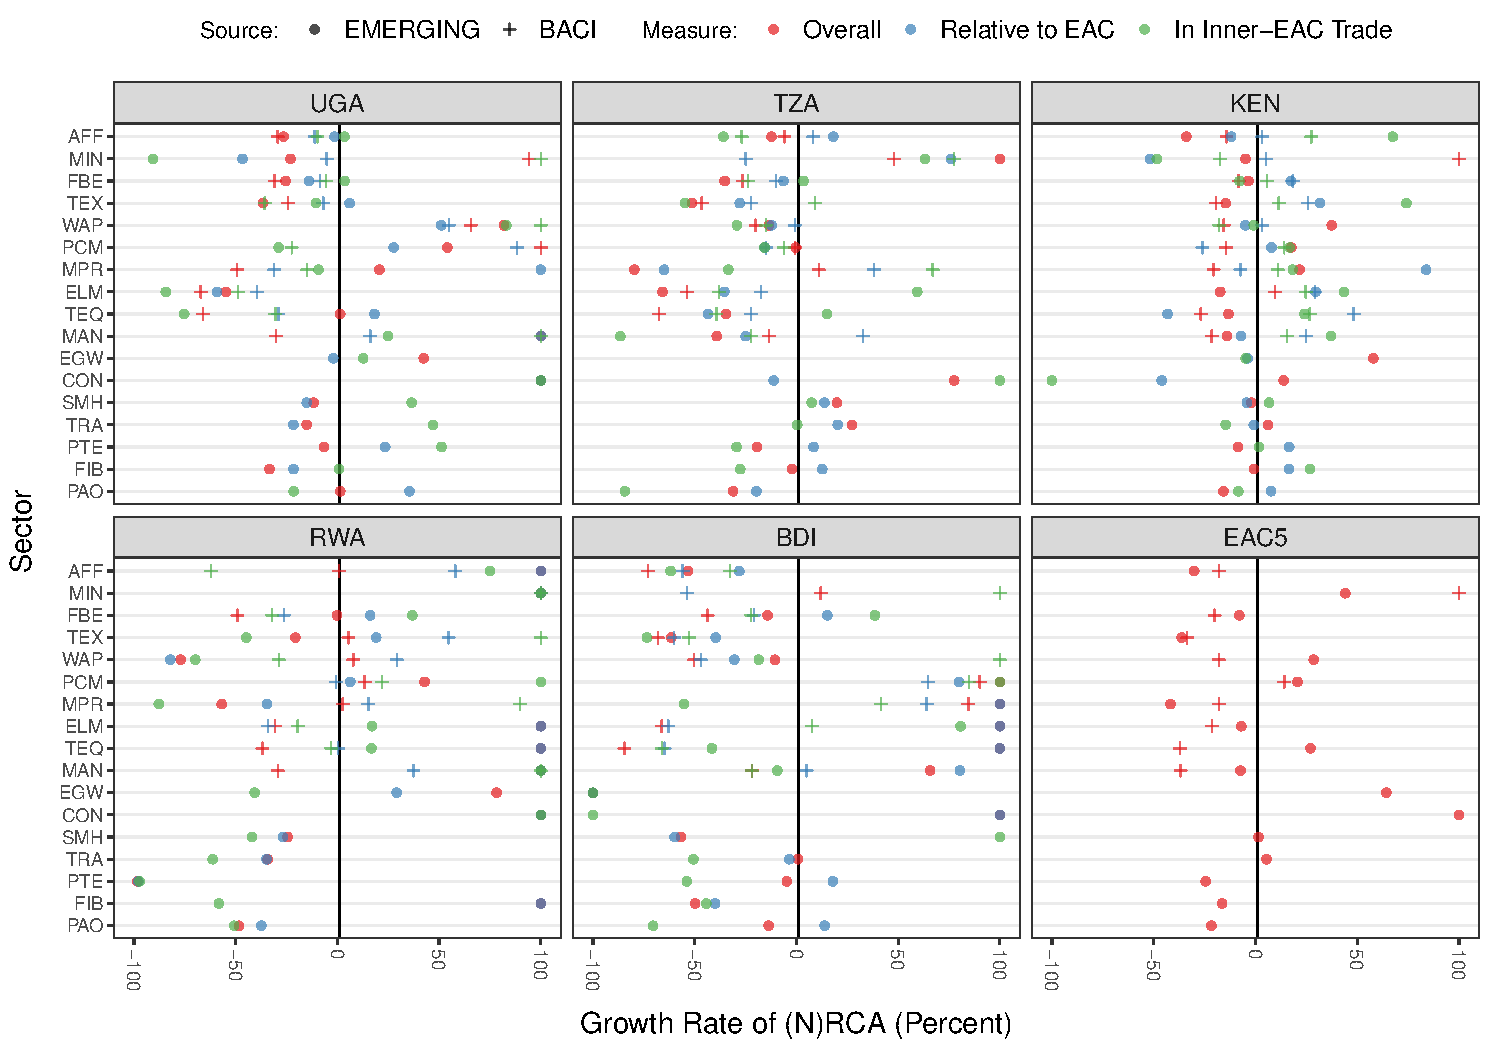
\includegraphics[width=1\textwidth]{"../Figures/REV/NRCA_EAC5_ALL_Growth.pdf"} \\ \raggedright
\scriptsize
\emph{Notes:} Figure shows the growth rate in percentage terms between the 2006-10 and 2015-19 (N)RCA medians. EM estimates are based on DVA in exports, BACI on gross exports. Appendix Figure \ref{fig:NRCA_Diff} and Table \ref{tab:NRCA_Diff} show the values. 
\end{figure}
\FloatBarrier



 
 
\section{Trade, Value Chains, and Economic Development}

Having extensively documented the patterns of EAC global and regional integration through both traditional trade (Section 3) and value chains (Section 4) while highlighting salient trends, potentials, imbalances, and policy priorities, a critical remaining policy questing regards the impact of different forms of integration on economic development in the region. This section attempts to provide causal reduced-form evidence on this matter following \citet{Kummritz20161}. 


\subsection{Review of the Empirical Literature}

The WDR Chapter 3 presents extensive correlational evidence that GVC participation is associated with gains in GDP per capita growth and labor productivity, poverty reduction, skill transfer, and employment creation, often benefiting gender equality, but also with challenges to taxation and higher inequality \citep{world2020trading, antras2022global}. The report highlights that long-term firm-to-firm links and specialization in GVC-related tasks promote efficient production, technology diffusion, and access to capital. A cross-country dynamic growth regression estimated with System-GMM yields an 11-14\% improvement in per-capita GDP following a 10\% increase in overall GVC participation, which is contrasted with a 2\% gain from increased trade in products fully produced in one country. Developing countries experience the biggest growth spurt upon transitioning from commodities to limited manufacturing, typically reaping 20\% income gains within 3 years. \newline

These findings are broadly echoed in much macroeconomic work on GVCs and economic development. Among the first, \citet{Kummritz20161} assesses the effect of GVC participation on labor productivity and DVA using OECD ICIOs for 61 countries and 34 industries from 1995-2011. He develops a novel instrumental variable (IV) for GVC participation - a VA trade resistance index combining third-country trade costs with industry-specific technological variables - and estimates that a 1 percent increase in VS leads to 0.11\% higher DVA in the average industry, and a 1 percent increase in VS1 leads to 0.60\% higher DVA and 0.33\% higher labor productivity. The effects of forward integration (VS1) are greater for high-income countries, whereas low/middle-income countries show stronger returns from backward integration (VS). \newline 

\citet{altomonte2018trade}, using an IV combining the growing size of container ships since 1997 with the ex-ante availability of deep sea ports, also present causal evidence of a positive effect of GVC-related trade (DVA in exports) on growth, which is larger than the effect of traditional trade. Both are three-step IV strategies following \citet{romer1999does} and \citet{feyrer2009distance, feyrer2019trade}. \newline 

\citet{constantinescu2019does}, used the WIOD with 40 countries and 13 sectors over 1995-2009, and find that (backward) GVC participation boosts labor productivity. An increase of 10\% yields an average productivity increase of 1.7\%. Examining a sample of 24 emerging economies, \citet{jangam2021does} show that both forward and backward participation significantly improve DVA in exports from 1995–2011. \citet{altun2023does} examine the role of GVC participation in high-technology exports for 120 countries during 1995–2019 and find that GVC participation correlates strongly with high-tech exports. \citet{kummritz2017economic} find that GVC participation increases VA, especially in upstream stages. \citet{pahl2020global} study the effects of GVC participation on VA in 58 countries (of which 38 developing) between 1970 and 2008 and find a robust positive effect on manufacturing productivity growth, especially for less productive countries where the distance to the global frontier is large. However, they find no positive effects on employment and some negative effects for middle-income countries. Thus, they conclude that GVC participation is a mixed blessing, inducing skill-biased technological change, in line with \citet{rodrik2018new}. \citet{Kummritz20161} notes that GVCs do not necessarily need to benefit developing countries as there could be adverse terms of trade effects or decreases in productive endowments from heavy engagement in them, which is also shown in some theoretical models such as \citet{baldwin2014trade}. An argument by \citet{kummritz2015global} is also that GVCs might substitute foreign for domestic suppliers. However, his empirical research suggests that FVA is a rather a complement to DVA. \newline   

 \citet{beverelli2019domestic} provide empirical evidence on the relationship between domestic value chains (DVCs) and GVCs. They find that across countries at different stages of development, higher domestic integration by 1 standard deviation raises GVC integration through backward linkages (VS) by 0.4\%. DVC integration explains up to 30\% of overall GVC participation. They explain these results with fixed costs of fragmentation and switching suppliers: "High fragmentation costs allow, due to their sunk nature, DVCs to act as stepping stones to GVCs" \citep{beverelli2019domestic}. \newline 
 
\citet{shen2021towards} construct a simple dynamic model to illustrate the micro-mechanism of industrial upgrading along the GVC. Using the WIOD, they find that more upstream industries correlate with higher profitability and VA, capital intensity, and R\&D investment. Their dynamic model explains this through three effects: endogenous sunk costs, decreasing intermediate input price elasticity, and sequential pricing effect uncertainty. They show that the empirical patterns revealed in China are consistent with the model's predictions. \citet{tian2022global} also study the relationship between GVC participation and industrial upgrading (process, product, and skill upgrading) using the WIOD. They find that GVC integration increases industrial upgrading for developing and developed countries. Developing countries benefit more from backward GVC participation through importing more sophisticated inputs and learning through embodied knowledge, whereas developed countries upgrade more through forward GVC participation. They interpret their findings as evidence against more critical voices and models questioning the benefits of developing country participation in GVCs, such as \citet{baldwin2014trade} or \citet{dalle2013industrial}. The macroeconomic study of \citet{lwesya2022integration} on GVCs and economic upgrading in the EAC, discussed in the introduction, also finds a significant positive effect of lagged FVA on DVA in EAC5 exports, with coefficients implying an elasticity of 0.49. \newline 

Many more microeconomic studies also find positive effects of GVC participation on industrial development. \citet{piermartini2014knowledge}, for example, use industry-level R\&D and patent data for a sample of 29 countries during 2000-2008 and show that knowledge spillovers increase with the intensity of supply chains linkages between countries and that these spillovers are larger than spillovers from traditional trade flows. Similar evidence is presented by \citet{benz2015trade}, who use firm-level data to show that offshoring leads to knowledge spillovers and that forward spillovers (from producers to users if intermediate inputs) are stronger than backward spillovers. \newline 

Microeconomic studies involving EAC members include \citet{barrientos2016shifting}'s case study of supermarket expansion within southern and eastern Africa, showing that higher quality and sourcing requirements by global and regional supermarket chains induced improved processes in Kenyan and Ugandan horticulture, allowing diversification and higher fruits and vegetable exports \citep{world2020trading}. A study of Kenyan horticulture by \citet{krishnan2018origin} shows that incomes increased after contract farmers adopted quality standards by their international buyers, and also that opportunistic RVCs emerged when suppliers found their produce rejected due to lack of standards compliance, which gradually led to more organized RVCs with own standards and procurement strategies. \citet{dihel2018does} study the effects of value chain participation on African farmers via a survey of 3,935 farmers, 60 aggregators, and 56 buyers in the maize, cassava, and sorghum value chains in Ghana, Kenya, and Zambia, and show that contracted farmers saw greater structural transformation, higher output, and better access to seeds, fertilizers, pesticides, technology, and extension services than non-contracted farmers. These findings are commensurate with \citet{daly2016maize}'s study of Maize value chains in East Africa, which identifies Kenyan processors as the lead firms demanding Ugandan suppliers to provide high-quality maize, and document investments into Ugandan production facilities by South African and German companies. They also document challenges in access to finance for farmers, insufficient commercial scale, and lack of communication of market signals and standards along the value chain.   


\subsection{Empirical Strategy}

A natural idea to assess the impact of GVC integration on economic development is to investigate if higher GVC participation is associated with higher domestic VA (GDP). Many authors do this in one form or another, including \citet{lwesya2022integration} who use DVA in exports. Following \citet{Kummritz20161} and \citet{rodriguez2000trade}, I argue that running regressions at the country level is subject to omitted variable bias from many factors affecting GVC integration and economic development. Thus, a sector-level regression framework with country-sector, country-year, and sector-year fixed effects is advantageous to capture many confounding factors such as infrastructure, geography, institutions, and economic policies, or multilateral resistance. A caveat is that the coefficients only capture within-industry effects, and are therefore likely lower bound estimates of the overall economic effects of GVC integration. My baseline specification is 
%
\begin{equation} \label{eq:VA_HDFE}
\log(\text{VA}_{cst}) = \beta \log(\text{GVC}_{cst}) + \alpha_{cs} + \beta_{ct} +\gamma_{st} + \epsilon_{cst},
\end{equation}
%
with $\text{GVC}_{cst}$ a GVC indicator (such as VS or VS1), and $\alpha_{cs}$, $\beta_{ct}$, and $\gamma_{st}$ country-sector, country-year, and sector-year fixed effects, respectively. The coefficient $\beta$ could still be biased by sector-level confounders, measurement error in $\text{GVC}_{cst}$, simultaneity, and reverse causality.  \newline

To address these issues, \citet{Kummritz20161} develops an instrument for GVC participation combining third-party trade costs and industry distance in the value chain to induce exogenous variation in FVA in exports, which forms the basis for simple GVC indicators. The first step is to predict the elements of the \textbf{VBE} (VA exports) matrix using exogenous trade costs and industry structure and then compute VS and VS1 indicators following Equations \ref{eq:VS} and \ref{eq:VS1} using this predicted matrix $\hat{\textbf{VBE}}$. These exogenous components $\hat{\text{VS}}_{uj}$ and $\hat{\text{VS1}}_{oi}$ can then be used to instrument VS and VS1 in Eq. \ref{eq:VA_HDFE}. Specifically, for each GVC instrument, a different $\hat{\textbf{VBE}}_t$ matrix is constructed, whose (time-varying) elements $vbe_{oiujt}$ are predicted using equations
%
\begin{align} \label{eq:predVS}
\log(\hat{vbe}_{oiujt}^\text{VS}) &= \beta^\text{VS} \log(\tau_{out}\times \delta_{oiuj}) + \alpha_{uj} + \beta_{ut} +\gamma_{jt} + \epsilon_{oiujt} \quad \forall\  u\neq o \\ \label{eq:predVS1}
\log(\hat{vbe}_{oiujt}^\text{VS1}) &= \beta^\text{VS1} \log(\tau_{out}\times \delta_{oiuj}) + \alpha_{oi} + \beta_{ot} +\gamma_{it} + \epsilon_{oiujt} \quad \forall\  o\neq u
\end{align}
%
to construct $\hat{\text{VS}}_{uj}$ and $\hat{\text{VS1}}_{oi}$, respectively.\footnote{E.g., $\hat{\text{VS}}_{ujt}$ is obtained by summing column $uj$ of a matrix $\hat{\textbf{VBE}}_t^\text{VS}$ where domestic elements are 0 and the non-domestic ($u\neq o$) elements are estimated using Eq. \ref{eq:predVS}, which includes fixed effects for the using country-sector ($uj$) and time ($ut$, $jt$) dimensions (as in the final model). Similarly, Eq. \ref{eq:predVS1} estimates $\hat{\textbf{VBE}}_t^\text{VS1}$ to obtain $\hat{\text{VS1}}_{oit}$. \vspace{-5mm} } Thus, all variation in the foreign sources of VA ($oit$) in Eq. \ref{eq:predVS} and in the usage ($ujt$) in Eq. \ref{eq:predVS1}, is due to the exogenous trade cost term: $\log(\tau_{out}\times \delta_{oiuj})$. \newline

The trade cost term has two components: $\tau_{out}$ is an export-weighted estimate of the bilateral trade costs of the supplier of VA ($o$) with all other trading partners ($k\neq u$) in period $t$. This is done to preserve the exogeneity of the trade cost measure to factors affecting the specific bilateral $ou$ link, which may be correlated with GVC-related trade along this link. Following \citet{Kummritz20161}, I use the World Bank ESCAP trade costs database \citep{arvis2016trade} based on \citet{novy2013gravity}, which provides a holistic, tariff-equivalent measure of total trade costs implied by an inverse gravity model. \newline 

The second term, $\delta_{oiuj}$, is a time-invariant measure of the distance between industries $oi$ and $uj$ along the GVC. It is defined as $\delta_{ijt} = 1/(u_{oi}\times d_{uj})$, where $u_{oi} = \frac{1}{T}\sum_t u_{oit}$ is the average upstreamness of country-sector $oi$ as defined in Eq. \ref{eq:upstreamness} and $d_{uj} = \frac{1}{T}\sum_t d_{ujt}$ a corresponding downstremness index, as described e.g. in \citet{antras2022global} and footnote \ref{fn:ds}. \citet{Kummritz20161} notes that the indirect trade costs ($\tau_{out}$) have a larger effect on VA for industries separated by more stages ($\delta_{oiuj}$). The index $\delta_{oiuj}$ is inverted since $u_{oi}$ and $d_{uj}$ have a positive relationship with the elements of \textbf{VBE}, to yield a trade cost index $\tau_{out}\times \delta_{oiuj}$ negatively related to $vbe_{oiujt}$.\footnote{\label{fn:IV}Unlike \citet{Kummritz20161}, I employ an industry distance measure ($\delta_{oiuj}$) at the country-sector level, whereas he uses a measure ($\delta_{ij}$) of pure industry distance that is averaged across countries as well. While this common technology assumption may be appropriate for his sample of mostly OECD economies in the OECD TIVA ICIO tables, the instrument constructed using this formulation lacks some relevance for the EAC5. This suggests that industries in developing countries use different technologies and have different GVC positions than the same industries in advanced economies. While using a bilateral-sector-level industry distance measure may partly compromise the exogeneity of the instrument, this is unlikely because this distance is still time-invariant, and the 2SLS regressions include triple fixed effects. Thus, the identifying variation still comes from time-variation in the trade cost term ($\tau_{out}$), and using a more accurate measure of industry distance merely helps increase the relevance of this term. Empirically, I find that computing two instruments using both $\delta_{oiuj}$ and $\delta_{ou}$, and including them both in the first stage often yields a sizeable improvement in the fit, indicating that the difference of local industry structure to the world average interacted with trade costs has some predictive power for FVA in developing countries. In all cases, however, the instruments are very weak.}\footnote{Another difference to \citet{Kummritz20161} is that I smooth bilateral trade costs using a centered 3-year MA and impute missing values at the end of the sample using the last MA observation carried forward. This is sensible because trade costs based on an inverted gravity model are endogenous to current trade flows and, therefore, more volatile than pure technological or regulatory changes would warrant. The smoothing step does not compromise the instrument's relevance, confirming that the ESCAP measure is noisy. Appendix Figure \ref{fig:ESCAP_EAC} shows the raw and smoothed bilateral trade costs among EAC5 members. Interestingly, the ESCAP estimates suggest that trading with Kenya is significantly less costly, and Kenya and Uganda also report trade costs below 100\% on each other. These costs are endogenous to observed trade flows, and the strong trade links between Kenya and Uganda have already been highlighted several times. However, this perspective entertains the possibility that high and asymmetric trading costs may be another reason for sluggish and asymmetric EAC integration in supply chain trade. In the framework of \citet{antras2020geography}, high trade costs imply greater importance for regional GVC participation. Since the IV trade cost measure ($\tau_{out}$) is a weighted average of origin's ($o$) trade costs with third parties, and EAC members trade much more with ROW than with each other, an accurate and timely representation of regional trade costs is irrelevant for the identification.} \newline

I also estimate economic returns to gross trade and trade in final goods. To instrument these, I omit the industry distance component and instead construct a sector-level time-varying 3rd-party trade cost measure $\tau_{oiut}$, obtained as exports-weighted average of sector $i$ in country $o$'s exports to all destination counties $k \neq u$. This is then used to predict bilateral sector-level trade in gross and final goods using similar zero-stage equations to \ref{eq:predVS} and \ref{eq:predVS1}, and the predictions are summed across importers to yield appropriate instruments for gross and final goods exports, respectively. \newline 

At last, I also consider returns to regional integration in both gross and VA terms using an alternative final stage model of the form
%
\begin{equation} \label{eq:VA_HDFE_RI}
\log(\text{VA}_{cst}) = \beta_1 \log(\text{GVC}_{cst}) + \beta_2 \text{SH}_{cst}^\text{EAC} \times \log(\text{GVC}_{cst}) + \alpha_{cs} + \beta_{ct} +\gamma_{st} + \epsilon_{cst},
\end{equation}
%
where $\text{SH}_{cst}^\text{EAC}$ is the EAC share in $\text{GVC}_{cst}$. Following Section 4.3, this is VS$^\text{EAC}$ and VS1$^\text{EAC}$ for GVC indicators and the EAC share in gross/final exports for traditional trade. The coefficient $\beta_2$ gives the additional impact when $\text{SH}_{cst}^\text{EAC}$ is increased by one unit (100\%), i.e., a 1\% increase in regional trade yields a $\beta_1+\beta_2$\% increase in VA, whereas a 1\% increase in extra-regional trade has an impact of $\beta_1$\%. Since the regional share is a component of $\text{GVC}_{cst}$, obtaining an instrument for it from the zero-stage predictions is straightforward. The RHS of the first stages thus mirror Eq. \ref{eq:VA_HDFE_RI}, with $\text{SH}_{cst}^\text{EAC}$ and $\text{GVC}_{cst}$ replaced by their zero-stage predicted measures. \newline

My default sample includes the full number of sectors (26 for EORA, 134 for EM) for 5 EAC countries: Uganda, Rwanda, Tanzania, Kenya, and Burundi.\footnote{South Sudan is omitted because of data quality concerns, Congo because of lacking RVC integration with the EAC, and different trading patterns. The inclusion of Congo does not significantly alter the results. \vspace{-5mm}} Estimations are run using indicators computed on EORA 2021, EORA 2015, and EM. With each database, I run one set of estimations using the full set of sectors and one using only manufacturing sectors (all sectors mapping to broad sectors FBE, TEX, WAP, PCM, MPR, ELM, TEQ, MAN, in Table \ref{tab:sec}). Unfortunately, with EM, all estimates are statistically insignificant and close to zero. This indicates that the high resolution of 134 sectors in these tables is not suitable for evaluating returns to trade and GVC participation in the EAC5. Aggregating to 17 broad sectors also yields insignificant results due to the short time dimension of 6 years. Thus, I do not report EM results. 


\subsection{Results: Gross Trade and Trade in Final Goods}

Table \ref{tab:FS_GT_RES} reports results for gross trade using the full sample of sectors, and Table \ref{tab:MS_GT_RES} shows identical regressions for the subset of manufacturing sectors. In both tables, the instruments are weak, and with one exception, not significantly different from OLS.\footnote{Appendix Table \ref{tab:ZS_FULL} shows the zero-stage regressions, with sizeable coefficients but weak within-$R^2$. } The OLS results suggest an elasticity of VA to gross trade of 0.13-0.25, in line with the 0.2 reported by the WDR. The results are also congruent to \citet{altomonte2018trade}, who find larger effects around 0.3 using the WIOD and very similar OLS and IV coefficients, with IV being slightly larger than OLS. The effects of trade in final goods on VA are slightly lower at 0.1-0.2, and the effects of both gross and final goods trade in manufacturing sectors (Table \ref{tab:MS_GT_RES}) are even lower at $\leq 0.1$. This indicates that intermediate trade, i.e., GVC-related trade, is more critical for economic development in the EAC, particularly for manufacturing sectors where intermediates account for a larger fraction of total trade. 


\begin{table}[h!] 
   \caption{\label{tab:FS_GT_RES} \textsc{Gross Trade EAC5 Regressions}}
   \centering
  \resizebox{\textwidth}{!}{
   \centering
   \begin{tabular}{lcccccccc}
      \tabularnewline \toprule
      Dependent Variable: & \multicolumn{8}{c}{log(VA)}\\ \cmidrule(lr){2-9}
      Exports Measure: & \multicolumn{4}{c}{Gross} & \multicolumn{4}{c}{Final Goods} \\ \cmidrule(lr){2-5} \cmidrule(lr){6-9}
      Data: & \multicolumn{2}{c}{EORA21} & \multicolumn{2}{c}{EORA15} & \multicolumn{2}{c}{EORA21} & \multicolumn{2}{c}{EORA15} \\ \cmidrule(lr){2-3} \cmidrule(lr){4-5} \cmidrule(lr){6-7} \cmidrule(lr){8-9}
      Model:                              & OLS    & IV            & OLS    & IV            & OLS    & IV    & OLS    & IV \\    
      \midrule
      \emph{Variables}\\
      log(E)                              & 0.2454$^{***}$ & 0.1072     & 0.1305$^{***}$ & 0.1503$^{*}$  & 0.1892$^{***}$   & 0.1931$^{**}$   & 0.1036$^{***}$   & 0.1776$^{**}$  \\   
                                          & (0.0419)       & (0.0770)              & (0.0233)       & (0.0777)      & (0.0353)    &  (0.0818)     &   (0.0207)    &  (0.0719) \\    
      \midrule
      \emph{Fixed-effects}\\
      \# country-sector                   & 130            & 130                   & 129            & 129                   & 130            & 130           & 129            & 129\\  
      \# country-year                     & 110            & 110                   & 80             & 80                    & 110            & 110           & 80             & 80\\  
      \# sector-year                      & 572            & 572                   & 416            & 416                   & 572            & 572           & 416            & 416\\  
            \midrule
      \emph{Fit statistics}\\
      Observations                        & 2,740          & 2,740                 & 2,023          & 2,023                 & 2,740          & 2,740         & 2,023          & 2,023\\  
      R$^2$                               & 0.9859         & 0.9856                & 0.9928         & 0.9928                & 0.9855         & 0.9855        & 0.9927         & 0.9927\\  
      Within R$^2$                        & 0.0485         & 0.0331                & 0.0238         & 0.0232                & 0.0269         & 0.0269        & 0.0143         & 0.0070\\  
      Wu-Hausman, p-value                 &                & 0.0101                &                & 0.5572                &                & 0.9703        &                & 0.0819\\  
      Kleibergen-Paap (1st stage), F &           & 23.99                 &                & 28.82                 &                & 3.086         &                & 20.28\\  
      Wald (1st stage), p-value   &                & $<0.001$              &                & $<0.001$              &                & 0.0790               &   & $<0.001$             \\  
      \bottomrule \\ [-0.9em]
      \multicolumn{9}{l}{\emph{Driscoll-Kraay (L=2) standard-errors in parentheses. Signif. Codes: ***: 0.01, **: 0.05, *: 0.1}}\\
      \multicolumn{9}{l}{\parbox{1.25\textwidth}{\scriptsize
\textit{Notes:} Table shows the elasticity of DVA to gross and final goods exports using EORA with full 26 sector resolution for 5 EAC countries: Uganda, Tanzania, Kenya, Rwanda, and Burundi. Estimations are done using both the first edition of EORA (EORA15: years 2000-2015) and the extended version (EORA21: years 2000-2021). The IV specification uses a sector-level exports weighted average of third-country trade costs as an instrument.  }}
   \end{tabular}
   }
\end{table}
\FloatBarrier


\begin{table}[h!] 
   \caption{\label{tab:MS_GT_RES} \textsc{Gross Trade EAC5 Regressions: Manufacturing Sectors}}
   \centering
  \resizebox{\textwidth}{!}{
   \centering
   \begin{tabular}{lcccccccc}
      \tabularnewline \toprule
      Dependent Variable: & \multicolumn{8}{c}{log(VA)}\\ \cmidrule(lr){2-9}
      Exports Measure: & \multicolumn{4}{c}{Gross} & \multicolumn{4}{c}{Final Goods} \\ \cmidrule(lr){2-5} \cmidrule(lr){6-9}
      Data: & \multicolumn{2}{c}{EORA21} & \multicolumn{2}{c}{EORA15} & \multicolumn{2}{c}{EORA21} & \multicolumn{2}{c}{EORA15} \\ \cmidrule(lr){2-3} \cmidrule(lr){4-5} \cmidrule(lr){6-7} \cmidrule(lr){8-9}
      Model:                              & OLS    & IV            & OLS    & IV            & OLS    & IV    & OLS    & IV \\    
      \midrule
      \emph{Variables}\\
      log(E)                              & 0.1015$^{***}$ & 0.9659      & 0.1175$^{***}$ & 0.2198      & -0.0566             & -0.1048            &  0.1075$^{***}$              & -0.0211  \\   
                                          & (0.0324)       & (0.6435)    & (0.0299)       & (0.1746)    & (0.0920)            & (0.5590)           & (0.0303)               &  (0.0400) \\   
      \midrule
      \emph{Fixed-effects}\\
      \# country-sector                   & 40           & 40                   & 40            & 40                   & 40            & 40           & 40            & 40\\  
     \# country-year                     & 110            & 110         & 80             & 80          & 110          & 110         & 80             & 80\\  
      \# sector-year                      & 176            & 176         & 128            & 128         & 176          & 176         & 128            & 128\\ 
            \midrule
      \emph{Fit statistics}\\
     Observations                        & 859            & 859         & 640            & 640         & 859          & 859         & 640            & 640\\  
      R$^2$                               & 0.9883         & 0.9817      & 0.9951         & 0.9951      & 0.9882       & 0.9882      & 0.9951         & 0.9950\\  
      Within R$^2$                        & 0.0077         & -0.5515     & 0.0216         & 0.0052      & 0.0022       & 0.0006      & 0.0216         & -0.0093\\  
      Wu-Hausman, p-value                 &                & 0.1060      &                & 0.7317      &              & 0.9675      &                & 0.5074\\  
      Kleibergen-Paap (1st stage), F &           & 1.009       &                & 5.278       &              & 0.4104      &                & 19.31\\ 
      Wald (1st stage), p-value   &                & 0.3152      &                & 0.0218             &                & 0.5217      &                & $<0.001$ \\  
      \bottomrule \\ [-0.9em]
      \multicolumn{9}{l}{\emph{Driscoll-Kraay (L=2) standard-errors in parentheses. Signif. Codes: ***: 0.01, **: 0.05, *: 0.1}}\\
       \multicolumn{9}{l}{\parbox{1.25\textwidth}{\scriptsize
\textit{Notes:} Table shows the elasticity of DVA to gross and final goods exports using EORA with a sample of 8 manufacturing sectors (FBE, TEX, WAP, PCM, MPR, ELM, TEQ, and MAN in Table \ref{tab:sec}), for 5 EAC countries: Uganda, Tanzania, Kenya, Rwanda, and Burundi. Estimations are done using both the first edition of EORA (EORA15: years 2000-2015) and the extended version (EORA21: years 2000-2021). The IV specification uses a sector-level exports weighted average of third-country trade costs as an instrument.  }}
   \end{tabular}
   }
\end{table}



\subsection{Results: Backward and Forward GVC Participation}

Appendix Table \ref{tab:ZS_FULL} reports the zero stage regressions predicting the elements $vbe_{oiujt}$. As expected, the trade cost measures correlate negatively with the elements of \textbf{VBE}. I then run both OLS and 2SLS fixed-effects regressions according to Eq. \ref{eq:VA_HDFE} using VS and VS1 measures in log-levels and instrumenting them with $\hat{\text{VS}}$ and $\hat{\text{VS1}}$, also in log-levels. I estimate 4 specifications: (1) OLS, (2) IV with a time-invariant ($\delta_{ij}$) industry-distance instrument as in \citet{Kummritz20161} (see Footnote \ref{fn:IV}), (2) IV with the bilateral ($\delta_{oiuj}$) industry-distance instrument, and (4) IV with both instruments. \newline

Table \ref{tab:FS_RES} shows the results on the full sample, and Table \ref{tab:MS_RES} for the manufacturing sample. Appendix Tables \ref{tab:FS_RES_F1} and \ref{tab:MS_RES_F1} report the corresponding first stages. The first stages are generally very weak, with many coefficients insignificant or of the wrong sign. Since the trade cost measure $\tau_{out}\times \delta_{oiuj}$ is negatively correlated with \textbf{VBE}, these negative first-stage coefficients could indicate some overfitting at the zero stages (Table \ref{tab:ZS_FULL}) which are also quite weak. In any case, this indicates that the IV/2SLS results in Tables \ref{tab:FS_RES} and \ref{tab:MS_RES} need to be treated with caution, even in cases where first-stage statistics at the bottom of these tables (such as a sizeable Kleinbergen \& Paap F-statistic) suggest that they are sufficiently strong. Also notable is that coefficients from the full EORA 200-2021 sample are generally smaller and more often insignificant than those of the WDR (EORA 2000-2015) sample. This appears to reflect a trend change in the data update from 2016 (the fixed effects absorb the structural break). Thus, I consider the results on the WDR sample more reliable, as its IO tables were created using a consistent methodology. 

\begin{table}[h!]
   \caption{\label{tab:FS_RES} \textsc{GVC Participation EAC5 Regressions}}
   \centering
  \resizebox{\textwidth}{!}{
   \begin{tabular}{lcccccccc}
      \tabularnewline \toprule
      Dependent Variable: & \multicolumn{8}{c}{log(VA)}\\ \cmidrule(lr){2-9}
      Data: & \multicolumn{4}{c}{EORA21 (2000-2021)} & \multicolumn{4}{c}{WDR EORA15 (2000-2015)} \\ \cmidrule(lr){2-5} \cmidrule(lr){6-9}
      Model:                  & OLS            & IV-$\delta_{ij}$      & IV-$\delta_{oiuj}$    & 2SLS               & OLS      & IV-$\delta_{ij}$      & IV-$\delta_{oiuj}$    & 2SLS\\  
      \midrule
      \emph{Variables}\\
      log(VS)                             & -0.2193$^{**}$     & 0.5786                & 0.6015                 & 0.2378$^{***}$         & -0.0664            & 0.2050$^{***}$         & 0.2096$^{***}$         & 0.1922$^{***}$\\   
                                          & (0.0841)           & (0.3895)              & (0.4202)               & (0.0827)               & (0.0539)           & (0.0418)               & (0.0412)               & (0.0435)\\ 
      \emph{Fit statistics}\\
      Observations                        & 2,740              & 2,740                 & 2,740                  & 2,740                  & 2,023              & 2,023                  & 2,023                  & 2,023\\  
      R$^2$                               & 0.9858             & 0.9776                & 0.9771                 & 0.9831                 & 0.9927             & 0.9919                 & 0.9918                 & 0.9920\\  
      Within R$^2$                        & 0.0416             & -0.5091               & -0.5413                & -0.1391                & 0.0066             & -0.1037                & -0.1075                & -0.0935\\  
      Wu-Hausman, p-value                 &                    & $<0.001$              & $<0.001$               & $<0.001$               &                    & $<0.001$               & $<0.001$               & $<0.001$\\   
      Kleibergen-Paap (1st stage), F      &                    & 1.652                 & 1.547                  & 32.23                  &                    & 47.22                  & 47.07                  & 53.78\\  
      Wald (1st stage), p-value &                              & 0.1988                & 0.2136                 & $<0.001$               &                    & $<0.001$               & $<0.001$               & $<0.001$\\ 
      \midrule
       \emph{Variables}\\
      log(E2R)                            & 0.7351$^{***}$     & 0.1842                & -0.1586                & -0.6351               & 0.7432$^{***}$     & 0.5716$^{***}$        & 0.5359$^{**}$          & 0.7366$^{***}$\\   
                                          & (0.0396)           & (1.129)               & (2.588)                & (2.591)               & (0.0607)           & (0.1831)              & (0.1907)               & (0.0597)\\   
      \emph{Fit statistics}\\
      Observations                        & 2,740              & 2,734                 & 2,733                  & 2,733                 & 2,023              & 2,017                 & 2,016                  & 2,016\\  
      R$^2$                               & 0.9950             & 0.9894                & 0.9803                 & 0.9608                & 0.9976             & 0.9973                & 0.9972                 & 0.9976\\  
      Within R$^2$                        & 0.6633             & 0.2889                & -0.3138                & -1.618                & 0.6683             & 0.6329                & 0.6164                 & 0.6724\\  
      Wu-Hausman, p-value                 &                    & 0.0678                & 0.0568                 & 0.0016                &                    & 0.0638                & 0.0460                 & 0.8330\\  
      Kleibergen-Paap (1st stage), F      &                    & 0.4409                & 0.1569                 & 0.2861                &                    & 3.421                 & 3.989                  & 4.301\\  
      Wald (1st stage), p-value           &                    & 0.5067                & 0.6920                 & 0.7512                &                    & 0.0645                & 0.0459                 & 0.0137\\  
      \midrule
      \emph{Fixed-effects}\\
      \# country-sector       & 130            & 130                   & 130                   & 130                   & 129      & 129                   & 129                   & 129\\  
      \# country-year         & 110            & 110                   & 110                   & 110                   & 80       & 80                    & 80                    & 80\\  
      \# sector-year          & 572            & 572                   & 572                   & 572                   & 416      & 416                   & 416                   & 416\\  
      \bottomrule \\ [-0.9em]
      \multicolumn{9}{l}{\emph{Driscoll-Kraay (L=2) standard-errors in parentheses. Signif. Codes: ***: 0.01, **: 0.05, *: 0.1}}\\
      \multicolumn{9}{l}{\parbox{1.25\textwidth}{\scriptsize
\textit{Notes:} Table shows the elasticity of DVA to backward (VS) and forward (E2R) GVC participation using EORA with full 26 sector resolution for 5 EAC countries: Uganda, Tanzania, Kenya, Rwanda, and Burundi. Estimations are done using both the first edition of EORA (EORA15: years 2000-2015) and the extended version (EORA21: years 2000-2021) via OLS and IV/2SLS. The IV models use exogenous GVC participation predicted by an exports-weighted average of third country trade costs interacted with bilateral ($\delta_ij$) or bilateral-sector level ($\delta_{oiuj}$) industry distance along the value chain as instruments. Appendix Table \ref{tab:ZS_FULL} shows the zero stage, and Table \ref{tab:FS_RES_F1} the first stage estimations, including the same set of triple fixed effects. }}
   \end{tabular}
   }
\end{table}
\FloatBarrier

Overall, the results suggest that GVC participation positively affects VA, and that this effect is larger for forward integration and manufacturing sectors (E2R $=$ VS1 is used here to avoid confusion). Drawing from the IV results in the WDR sample, a 1\% increase in the foreign content of exports (VS) implies a 0.2\% increase in VA in the full sample, and a 0.45-0.5\% increase in manufacturing VA. On the other hand, a 1\% increase in the re-exported content of exports (E2R) implies a 0.5-0.7\% increase in VA, and a 0.8-1\% increase in manufacturing VA. 

\begin{table}[h!]
   \caption{\label{tab:MS_RES} \textsc{GVC Participation EAC5 Regressions: Manufacturing Sectors}}
   \centering
  \resizebox{\textwidth}{!}{
   \begin{tabular}{lcccccccc}
      \tabularnewline \toprule
      Dependent Variable: & \multicolumn{8}{c}{log(VA)}\\ \cmidrule(lr){2-9}
      Data: & \multicolumn{4}{c}{EORA21 (2000-2021)} & \multicolumn{4}{c}{WDR EORA15 (2000-2015)} \\ \cmidrule(lr){2-5} \cmidrule(lr){6-9}
      Model:                  & OLS            & IV-$\delta_{ij}$      & IV-$\delta_{oiuj}$    & 2SLS               & OLS      & IV-$\delta_{ij}$      & IV-$\delta_{oiuj}$    & 2SLS\\  
      \midrule
      \emph{Variables}\\
     log(VS)                            & 0.1344$^{***}$     & 1.404                 & 1.638                  & 0.4800$^{**}$          & 0.0590$^{*}$       & 0.4394$^{***}$         & 0.4562$^{***}$         & 0.2089$^{***}$\\   
                                          & (0.0227)           & (1.945)               & (2.768)                & (0.1835)               & (0.0291)           & (0.1178)               & (0.1247)               & (0.0459)\\   
      \emph{Fit statistics}\\
      Observations                        & 859                & 859                   & 859                    & 859                    & 640                & 640                    & 640                    & 640\\  
      R$^2$                               & 0.9884             & 0.9685                & 0.9605                 & 0.9870                 & 0.9951             & 0.9940                 & 0.9939                 & 0.9949\\  
      Within R$^2$                        & 0.0190             & -1.674                & -2.356                 & -0.1064                & 0.0054             & -0.2179                & -0.2381                & -0.0293\\  
      Wu-Hausman, p-value                 &                    & 0.0974                & 0.1160                 & 0.0010                 &                    & 0.0025                 & 0.0028                 & 0.0249\\  
      Kleibergen-Paap (1st stage), F                    &                    & 0.4762                & 0.3118                 & 51.79                  &                    & 61.77                  & 62.66                  & 24.34\\ 
      Wald (1st stage), p-value &                   & 0.4901                & 0.5765                 & $<0.001$  &                    & $<0.001$  & $<0.001$   & $<0.001$\\
      \midrule
       \emph{Variables}\\
      log(E2R)                            & 0.6724$^{***}$     & 0.8149$^{***}$        & 0.8204$^{***}$         & 0.8366$^{***}$         & 0.5275$^{***}$     & 1.094$^{***}$         & 1.214$^{***}$          & 0.7602$^{**}$\\   
                                          & (0.0775)           & (0.0377)              & (0.0390)               & (0.0443)               & (0.1523)           & (0.3019)              & (0.3362)               & (0.2842)\\  
      \emph{Fit statistics}\\
      Observations                        & 859                & 859                   & 859                    & 859                    & 640                & 640                   & 640                    & 640\\  
      R$^2$                               & 0.9966             & 0.9963                & 0.9962                 & 0.9961                 & 0.9978             & 0.9946                & 0.9932                 & 0.9972\\  
      Within R$^2$                        & 0.7148             & 0.6827                & 0.6801                 & 0.6721                 & 0.5496             & -0.0841               & -0.3807                & 0.4427\\  
      Wu-Hausman, p-value     &                    & 0.0002                 & $<0.001$               & $<0.001$               &                    & 0.1988                & 0.1378                 & 0.5741\\  
     Kleibergen-Paap (1st stage), F                     &                    & 7.529                 & 9.387                  & 22.39                  &                    & 11.86                 & 9.076                  & 7.092\\  
      Wald (1st stage), p-value &                    & 0.0062                & 0.0022                 & $<0.001$  &                    & 0.0006                & 0.0027                 & 0.0009\\ 
      \midrule
      \emph{Fixed-effects}\\
      \# country-sector       & 40                 & 40                    & 40                     & 40                    & 40                 & 40                    & 40                     & 40\\  
      \# country-year         & 110                & 110                   & 110                    & 110                   & 80                 & 80                    & 80                     & 80\\  
      \# sector-year          & 176                & 176                   & 176                    & 176                   & 128                & 128                   & 128                    & 128\\ 
      \bottomrule \\ [-0.9em]
      \multicolumn{9}{l}{\emph{Driscoll-Kraay (L=2) standard-errors in parentheses. Signif. Codes: ***: 0.01, **: 0.05, *: 0.1}}\\
      \multicolumn{9}{l}{\parbox{1.25\textwidth}{\scriptsize
\textit{Notes:} Table shows the elasticity of DVA to backward (VS) and forward (E2R) GVC participation using EORA with a sample of 8 manufacturing sectors (FBE, TEX, WAP, PCM, MPR, ELM, TEQ, and MAN in Table \ref{tab:sec}), for 5 EAC countries: Uganda, Tanzania, Kenya, Rwanda, and Burundi. Estimations are done using both the first edition of EORA (EORA15: years 2000-2015) and the extended version (EORA21: years 2000-2021) via OLS and IV/2SLS. The IV models use exogenous GVC participation predicted by an exports-weighted average of third country trade costs interacted with bilateral ($\delta_ij$) or bilateral-sector level ($\delta_{oiuj}$) industry distance along the value chain as instruments. Appendix Table \ref{tab:ZS_FULL} shows the zero stage, and Table \ref{tab:FS_RES_F1} the first stage estimations, including the same set of triple fixed effects. }}
   \end{tabular}
   }
\end{table}
\FloatBarrier

Larger productivity gains from forward integration are also prevalent in the literature. \citet{Kummritz20161} finds robust benefits of GVC backward and forward integration on VA in both developing and developed countries, with a larger benefit of forward integration (E2R) at elasticities of 0.58 for low/middle-income countries and 0.68 for high-income countries. VS elasticities are smaller around 0.09/0.21, respectively. He also estimates labor productivity elasticities to E2R of 0.29 for low/middle-income countries and 0.49 for high-income countries. In a similar exercise, \citet{kummritz2015global} finds that high-income countries benefit relatively more from forward linkages, whereas middle-income countries also benefit from backward linkages (VS). The results presented here broadly align with these findings, suggesting that both backward and forward integration have sizeable returns in low-income countries. In manufacturing sectors, the estimates for these EAC countries are even greater than those of \citet{Kummritz20161}, with VA elasticities from forward integration close to 1, tentatively indicating that low-income African economies (not covered by the OECD TIVA ICIO's) can benefit substantially from increasing their supply of high-quality manufacturing intermediates. I note that these estimates, while large, are still smaller than the 1.1-1.4 elasticities to overall GVC participation (VS + VS1) reported by the WDR. 
 


\subsection{Results: Regional Integration}

Tables \ref{tab:FS_RI_GT_RES} and \ref{tab:FS_RI_RES} show regional integration estimations for gross and GVC-related trade using the full sample of sectors. Appendix Tables \ref{tab:MS_RI_GT_RES} and \ref{tab:MS_RI_RES} provide equivalent results for manufacturing sectors. In the manufacturing sample, the interaction term is statistically insignificant. \newline 

In this more complex specification, the instruments are even weaker, thus, for GVC-related trade, I only report 2SLS specifications employing both sets of instruments. With gross trade (Table \ref{tab:FS_RI_GT_RES}), the Wu-Hausmann test fails to reject the exogeneity of the regressor in all but the first IV specification. With GVC-related trade (Table \ref{tab:FS_RI_RES}) this is also the case for forward integration. For backward integration, the IV specifications have a sizeable negative within-$R^2$ and a huge negative interaction effect. This signifies that the instruments are useless in this more complex case. Therefore, I only interpret the OLS estimates. \newpage 

Table \ref{tab:FS_RI_GT_RES} reports positive interaction terms with significant coefficients between 0.066 and 0.079, suggesting that an increase in regional trade in both gross terms and in final goods yields a 6-8 pp. higher VA return than an increase in extra-regional trade, whose VA return to a doubling of exports is estimated between 10\% and 24\%. The empirical results thus suggest that regional integration through trade is beneficial for economic growth in the region.  

\begin{table}[h!]
   \caption{\label{tab:FS_RI_GT_RES} \textsc{EAC5 Regional Integration via Gross Trade Regressions}}
   \centering
  \resizebox{\textwidth}{!}{
   \centering
   \begin{tabular}{lcccccccc}
      \tabularnewline \toprule
      Dependent Variable: & \multicolumn{8}{c}{log(VA)}\\ \cmidrule(lr){2-9}
      Exports Measure: & \multicolumn{4}{c}{Gross} & \multicolumn{4}{c}{Final Goods} \\ \cmidrule(lr){2-5} \cmidrule(lr){6-9}
      Data: & \multicolumn{2}{c}{EORA21} & \multicolumn{2}{c}{EORA15} & \multicolumn{2}{c}{EORA21} & \multicolumn{2}{c}{EORA15} \\ \cmidrule(lr){2-3} \cmidrule(lr){4-5} \cmidrule(lr){6-7} \cmidrule(lr){8-9}
      Model:                      & OLS    & IV            & OLS    & IV            & OLS    & IV    & OLS    & IV \\    
      \midrule
      \emph{Variables}\\
      log(E)                                         & 0.2361$^{***}$ & 0.0290                 & 0.1034$^{***}$ & 0.1051                  & 0.1718$^{***}$ & -0.1314                & 0.0837$^{***}$ & 0.2198$^{**}$ \\   
                                                     & (0.0463)       & (0.0910)               & (0.0202)       & (0.0988)                & (0.0378)       & (0.3728)               & (0.0195)       & (0.1026) \\   
      log(E) $\times$ SH$^\text{EAC5}$               & 0.0555         & 0.0661$^{***}$         & 0.0749$^{**}$  & 0.0468                  & 0.0787$^{***}$ & 0.1437                 & 0.0531         & -0.0397  \\     
                                                     & (0.0405)       & (0.0174)               & (0.0279)       & (0.0309)                & (0.0260)       & (0.0898)               & (0.0335)       & (0.0352)  \\  
      \midrule
      \emph{Fixed-effects}\\
      \# country-sector                              & 130            & 130                    & 129            & 129                     & 130            & 130                    & 129            & 129\\  
      \# country-year                                & 110            & 110                    & 80             & 80                      & 110            & 110                    & 80             & 80\\  
      \# sector-year                                 & 572            & 572                    & 416            & 416                     & 572            & 572                    & 416            & 416\\ 
            \midrule
      \emph{Fit statistics}\\
      Observations                                   & 2,740          & 2,740                  & 2,023          & 2,023                   & 2,740          & 2,740                  & 2,023          & 2,023\\  
      R$^2$                                          & 0.9859         & 0.9854                 & 0.9929         & 0.9929                  & 0.9856         & 0.9846                 & 0.9928         & 0.9926\\  
      Within R$^2$                                   & 0.0507         & 0.0166                 & 0.0307         & 0.0296                  & 0.0325         & -0.0340                & 0.0181         & -0.0071\\  
      Wu-Hausman, p-value                            &                & 0.0001                 &                & 0.4127                  &                & 0.2302                 &                & 0.2113\\
      \bottomrule \\ [-0.9em]
      \multicolumn{9}{l}{\emph{Driscoll-Kraay (L=2) standard-errors in parentheses. Signif. Codes: ***: 0.01, **: 0.05, *: 0.1}}\\
      \multicolumn{9}{l}{\parbox{1.19\textwidth}{\scriptsize
\textit{Notes:} Table reports analogous estimations to Table \ref{tab:FS_GT_RES}, but now including an interaction term of the log of exports with the regional share in exports, which captures the additional returns from a regional expansion in trade. }}
   \end{tabular}
   }
\end{table}
\FloatBarrier


Table \ref{tab:FS_RI_RES} indicates a significant positive OLS interaction term for forward GVC integration of order 0.13-0.14, implying that a 100\% increase in forward integration through regional trade yields a 13-14 pp. higher return than the already sizeable return of 73\% to extra-regional forward linkages. For backward integration, the terms on the OLS regression are negative of order 0.14-0.19, but the main effects are also negative. Since backward integration is particularly prone to simultaneity, as evident from Tables \ref{tab:FS_RES} and \ref{tab:MS_RES}, a strong instrument is needed for identification, so these OLS coefficients are likely not very meaningful. Further work is required to create stronger instruments for GVC participation in developing countries. 


\begin{table}[h!]
   \caption{\label{tab:FS_RI_RES} \textsc{EAC5 Regional Integration via RVCs Regressions}}
   \centering
  \resizebox{\textwidth}{!}{
   \centering
   \begin{tabular}{lcccccccc}
      \tabularnewline \toprule
      Dependent Variable: & \multicolumn{8}{c}{log(VA)}\\ \cmidrule(lr){2-9}
      GVC Indicator: & \multicolumn{4}{c}{Backward Integration (VS)} & \multicolumn{4}{c}{Forward Integration (E2R)} \\ \cmidrule(lr){2-5} \cmidrule(lr){6-9}
      Data: & \multicolumn{2}{c}{EORA21} & \multicolumn{2}{c}{EORA15} & \multicolumn{2}{c}{EORA21} & \multicolumn{2}{c}{EORA15} \\ \cmidrule(lr){2-3} \cmidrule(lr){4-5} \cmidrule(lr){6-7} \cmidrule(lr){8-9}
      Model:                      & OLS    & 2SLS            & OLS    & 2SLS            & OLS    & 2SLS    & OLS    & 2SLS \\    
      \midrule
      \emph{Variables}\\
      log(GVC)                                       & -0.1926$^{**}$ & 0.1478$^{***}$         & -0.0605      & 0.0832$^{**}$           & 0.7335$^{***}$ & 0.7110$^{***}$ & 0.7315$^{***}$ & 0.7467$^{***}$ \\    
                                                     & (0.0883)       & (0.0481)               & (0.0629)     & (0.0373)                & (0.0398)       & (0.1008)       & (0.0646)       & (0.1925) \\  
      log(GVC) $\times$ SH$^\text{EAC5}$             & -0.1869$^{*}$  & -1.116$^{***}$         & -0.1397      & -1.960$^{*}$            & 0.1332$^{***}$ & 0.6306         & 0.1383$^{*}$   & 0.0082  \\    
                                                     & (0.1015)       & (0.2550)               & (0.2464)     & (1.038)                 & (0.0280)       & (0.6673)       & (0.0754)       & (0.5347)  \\                                                           
      \midrule
      \emph{Fixed-effects}\\
      \# country-sector                              & 130            & 130                    & 129          & 129                     & 130            & 130            & 129            & 129\\  
      \# country-year                                & 110            & 110                    & 80           & 80                      & 110            & 110            & 80             & 80\\  
      \# sector-year                                 & 572            & 572                    & 416          & 416                     & 572            & 572            & 416            & 416\\
            \midrule
      \emph{Fit statistics}\\
      Observations                                   & 2,740          & 2,740                  & 2,023        & 2,023                   & 2,740          & 2,733          & 2,023          & 2,016\\  
      R$^2$                                          & 0.9858         & 0.9837                 & 0.9927       & 0.9917                  & 0.9950         & 0.9948         & 0.9976         & 0.9976\\  
      Within R$^2$                                   & 0.0459         & -0.0980                & 0.0074       & -0.1300                 & 0.6648         & 0.6502         & 0.6717         & 0.6731\\  
      Wu-Hausman, p-value                            &                & $<0.001$  &              & $<0.001$    &                                         & 0.4314         &                & 0.7855\\ 
      \bottomrule \\ [-0.9em]
      \multicolumn{9}{l}{\emph{Driscoll-Kraay (L=2) standard-errors in parentheses. Signif. Codes: ***: 0.01, **: 0.05, *: 0.1}}\\
     \multicolumn{9}{l}{\parbox{1.19\textwidth}{\scriptsize
\textit{Notes:} Table reports analogous estimations to Table \ref{tab:FS_RES}, but now including an interaction term of the log of GVC participation (VS or E2R) with its regional share, which captures the additional returns from a regional expansion in GVC participation. Due to the weakness of the instruments, only the 2SLS specification, including both instrumental variables and their respective interaction terms, is reported. }}
   \end{tabular}
   }
\end{table}
\FloatBarrier



\section{Summary and Conclusion} 

Using rich and novel data sources, this study rigorously examines the EAC region's global and regional integration through trade and value chains and their effects on economic development. The analysis focusses on five member countries: Uganda, Tanzania, Kenya, Rwanda, and Burundi. \newline

Several salient patterns stand out. The first is that, exempting a small COVID-related rebound in the share of regional trade, the region is not integrating deeper through gross trade. This is particularly the case for imports, where the EAC share with itself has declined from 10\% in 2000 to 7.5\% in 2020, while the export share remained constant at around 17\%. However, this decline is mainly driven by manufacturing and masks increasing regional trade shares in agriculture, forestry and fishing (AFF) and processed foods and beverages (FBE). Considering total trade (exports+imports), AFF trade with ROW was 10x greater than inner-EAC trade in 2020, down from 40x in 2000. In FBE, this ratio declined from 16x (2000) to 11x (2020). In manufacturing, it increased from 15x (2000) to 20x (2020). Manufacturing trade accounts for 64\% of EAC5 goods trade, versus  8.1\% (AFF), 15\% (FBE), and 13\% (mining), and thus drives aggregate patterns. \newline 

EAC members assume different roles in regional trade. Kenya is a dominant regional exporter, particularly of manufactured products, where 40\% of its exports are regional, but only a moderate importer: 18\% of Kenyan agricultural imports and less than 1\% of its manufacturing imports come from the region. Tanzania also imports little from the region, only 5\% of AFF/FBE and 3\% of manufacturing imports. It has regional export shares between 20\% (AFF) and 11\% (FBE). The smaller economies are much more integrated, with regional export and import shares generally above 20\%. Particularly Uganda is becoming a significant regional exporter in AFF and FBE, with regional export shares between 35 and 40\%. Burundi also recently became a strong agricultural exporter, at a regional share rising from 5\% in 2005 to 60\% in 2020. \newline

This suggest that regional integration is unequal and follows a pattern where countries first become regional agricultural exporters and then exporters of limited manufactures. However, these manufactures do not significantly cater to a large share of regional demand and thus do not drive regional integration as manufacturers become more foreign-oriented. The FBE sector is intermediate between these two and shows greater promise for regional integration. \newline

In value added (VA) terms, all members have a foreign content share (VS) between 10\% (Kenya) and 30\% (Congo). The EU and China are the greatest suppliers of EAC foreign content. Only Uganda, Rwanda, and Burundi have a high regional share in VS of 15-30\%. The largest regional supplier is Kenya, mostly of manufacturing inputs, followed by Uganda as a regional supplier of mostly primary agriculture. EAC sectors with the highest regional VS shares are FBE and sale and repair of vehicles, fuel trade and hotels (SMH) at 14\% each. Petrochemicals (PCM) and textiles (TEX) also have EAC VS shares of 7-9\%. Core manufacturing sectors with overall high VS have small regional shares, such as electrical machinery (ELM), where VS in the EAC is at 35\%, but the regional share in VS is only 2.8\%. EAC regional integration in supply chains thus concentrates on food processing and light manufacturing but at low regional VS shares. This highlights both the great potential and significant challenges in deepening manufacturing RVCs.  \newline

For forward GVC participation (re-exported exports or VS1), the EU is the major GVC partner. Regional forward integration is still in its infancy, at regional VS1 shares below 6\% in all EAC members. The strongest forward linkages are between Kenya and Uganda, with Uganda accounting for 4.4\% of Kenya's VS1 (approx. 80 million USD) and Kenya accounting for 3.2\% of Ugandan VS1 (approx. 30 million USD). At the sector level, 21\% of agriculture and manufacturing exports are re-exported, followed by 15\% of mining exports and 13\% of FBE. Bilaterally, 54\% of Kenyan VS1 through Uganda are manufacturing inputs, whereas 45\% of Ugandan VS1 through Kenya are agricultural inputs, highlighting the different roles of these two countries in RVCs. 21\% of Kenyan manufacturing VS1 is via its EAC partners, indicating that the supply of regional manufacturing inputs is quantitatively important for Kenya. Considering overall EAC VS1 by sector, the highest regional shares are in manufacturing and FBE at 6.7\% each, followed by AFF at 4\%. Regional forward linkages are thus much weaker than backward linkages, which, in FBE, are twice as large. \newline

The region does not seem to be integrating deeper into GVCs. Backward linkages (VS) show some improvements in the 3 smaller economies in recent years, countered by a slight decline in the larger economies. Forward linkages (VS1) exhibit a very weak decline. Unlike gross trade, the regional VS share is growing at a slow pace of 0.5 pp. per year, and regional shares in VS1 and VA imports (both gross and final) are growing at 0.2 pp./year. Regional integration is advancing in all sectors, but particularly fast in FBE, at rates above 0.5 pp./year on all metrics. Growth in regional VS1 shares in FBE is also particularly equitable, whereas in core manufacturing, which is integrating in VS and VS1 at 0.25 pp./year, the growth in regional VS1 is entirely driven by Kenya, with other countries experiencing losses. The analysis thus highlights the potential of the FBE sector and challenges fostering more horizontal manufacturing RVCs between members. \newline

Examining the evolving position of EAC sectors in GVCs indicates a downstream shift in all members and sectors, implying a move towards production stages closer to final demand running against the global trend towards longer GVCs. For AFF and FBE, this appears to be good news as it implies more local value addition. For manufacturing sectors, on the other hand, it indicates a shift towards processing trade rather than high-quality intermediates. The transport and tourism (TRA) sector in Kenya also saw a downstream shift, suggesting some local upgrading. \newline

Computing (New) Revealed Comparative Advantage indices signifies that all members and the region as a whole have sizeable (N)RCA in AFF (4.2) and FBE (5) and a strong disadvantage in core manufacturing (below 0.1 in ELM and TEQ). The region also has (N)RCA in travel services (TRA) of 2.8, particularly Kenya (3.1) and Tanzania (3). Relative to the region, Kenya has slight (N)RCA in most manufacturing sectors apart from PCM, where Tanzania and Rwanda perform strongly. Uganda, Kenya, and Burundi have regional (N)RCA in FBE, Kenya and Tanzania in tourism (TRA), and Uganda in electricity supply (EGW). Except for the latter, these estimates are below 2 and thus moderate. They may nevertheless require policy attention, particularly in manufacturing where Kenya has gained relatively. Trends also signify a slight overall EAC (N)RCA loss in AFF and FBE, encouraging policy efforts to increase foods production and exports. \newline

OLS and IV estimates imply that EAC integration through trade and GVCs benefits sector-level economic growth at elasticities of VA to gross exports of 0.13-0.25 and 0.1-0.2 to exports of final goods. This suggests that intermediates trade is more important for economic development than trade in final goods. Manufacturing sectors show lower returns to gross trade. Examining GVC participation yields IV estimates of 0.2 (all sectors) and 0.45 (manufacturing sectors) to backward GVC participation (VS) and 0.6 (all sectors) and 0.9 (manufacturing sectors) to forward GVC participation (VS1/E2R). These resonate with other papers and the 2020 World Development Report finding that GVC participation benefits economic development, particularly forward linkages in manufacturing. The paper also investigates the returns of deeper regional integration vis-a-vis global integration. OLS estimates suggest that deeper regional linkages yield additional returns: The elasticity to gross and final goods exports increases by 0.06-0.08 for regional trade, and the elasticity to forward GVC participation (VS1) increases by 0.13-0.14 for regional links.  \newline 

The paper thus highlights both prospects of and challenges to EAC regional integration. The region demonstrates a modest level of integration through trade and RVCs, which are concentrated in certain sectors. In particular, the FBE sector demonstrates higher levels of regional integration and growth. At the same time, integration in manufacturing is concentrating on Kenya's role as a supplier of inputs, with a limited supplier role of other countries. There is no clear trend towards greater regional integration through gross trade, and the pace of integration in VA trade, while positive, is very slow. Shifts in comparative advantage suggest a loss of (N)RCA in manufacturing, including FBE, alongside a downstream shift. This should prompt policy action to at least increase output and deepen RVCs in the FBE sector. Broader industrial policy coordination may also be necessary to mitigate Kenya's increasing role as a regional manufacturing hegemon. Sector-level estimates suggest that integration through trade and GVCs benefits domestic activity, particularly within RVCs. Thus, any policy action should be considerate not to slow down or reverse the (already sluggish) trend towards increased EAC regional integration through RVCs. \newline 

Regarding the AfCFTA, this study shows that establishing a common market among economies with different distributions of comparative advantage may result in vertical GVCs and RVCs, leading to a loss of competitiveness in certain sectors and countries, particularly in smaller manufacturing sectors. Thus coordination of industrial and GVC-related policies should be considered together with the planned protocols to establish and regulate a common African market. 




\newpage
\bibliographystyle{apacite}
\bibliography{GVC}


\newpage
\section*{Appendix}

The appendix has two parts: Part A provides additional concordances for countries and sectors to their corresponding aggregates and EORA data quality reports; Part B provides additional tables and figures, many of which are referred to from the main text. 


\subsection*{A. Data Aggregation and EORA Quality Reports}
\setcounter{table}{0}
\renewcommand{\thetable}{A\arabic{table}}
\setcounter{figure}{0}
\renewcommand{\thefigure}{A\arabic{figure}}

\begin{table}[h!] \vspace{-4mm}
\centering
\caption{\textsc{Countries and Regions}}
\label{tab:ctrydet}
\vspace{2mm}
\resizebox{0.85\textwidth}{!}{
\begin{tabular}{llp{6cm}} \toprule
\textit{Region} & \textit{Description} & \textit{Countries} \\ \midrule
EAC & East African Community & UGA, TZA, KEN, RWA, BDI, COD, SSD \\ \\
SSA & Sub-Saharan Africa (Excluding EAC) & AGO, BEN, BFA, BWA, CAF, CIV, CMR, COG, COM, CPV, ERI, ETH, GAB, GHA, GIN, GMB, GNB, GNQ, LBR, LSO, MDG, MLI, MOZ, MRT, MUS, MWI, NAM, NER, NGA, SDN, SEN, SLE, SOM, STP, SWZ, SYC, TCD, TGO, ZAF, ZMB, ZWE \\ \\
EUU & European Union + GBR & AUT, BEL, BGR, CYP, CZE, DEU, DNK, ESP, EST, FIN, FRA, GBR, GRC, HRV, HUN, IRL, ITA, LTU, LUX, LVA, NLD, POL, PRT, ROU, SVK, SVN, SWE, MLT \\ \\
ECA & Europe and Central Asia (Non-EU) & ALB, AND, ARM, AZE, BIH, BLR, CHE, CHI, FRO, GEO, GIB, GRL, IMN, ISL, KAZ, KGZ, LIE, MCO, MDA, MKD, MNE, NOR, RUS, SMR, SRB, TJK, TKM, TUR, UKR, UZB, XKX \\ \\
MEA & Middle East and North Africa & ARE, BHR, DJI, DZA, EGY, IRN, IRQ, ISR, JOR, KWT, LBN, LBY, MAR, OMN, PSE, QAT, SAU, SYR, TUN, YEM \\ \\
NAC & North America and Canada & BMU, CAN, USA \\ \\
LAC & Latin America and Carribean & ABW, ARG, ATG, BHS, BLZ, BOL, BRA, BRB, CHL, COL, CRI, CUB, CUW, CYM, DMA, DOM, ECU, GRD, GTM, GUY, HND, HTI, JAM, KNA, LCA, MAF, MEX, NIC, PAN, PER, PRI, PRY, SLV, SUR, SXM, TCA, TTO, URY, VCT, VEN, VGB, VIR \\ \\
ASE & ASEAN & BRN, IDN, KHM, LAO, MMR, MYS, PHL, SGP, THA, VNM \\ \\
SAS & South Asia & AFG, BGD, BTN, IND, LKA, MDV, NPL, PAK \\ \\
CHN & China & CHN, HKG, TWN \\ \\
ROA & Rest of Asia & ASM, GUM, JPN, KOR, MAC, MNG, MNP, NCL, PRK, PYF, TLS \\ \\
OCE & Oceania & AUS, FJI, FSM, KIR, MHL, NRU, NZL, PLW, PNG, SLB, TON, TUV, VUT, WSM
 \\ \bottomrule
\end{tabular}
}
\vspace{-1.5cm}
\end{table}
\FloatBarrier


\begin{table}[ht]
\centering
\caption{\label{tab:EMSec} EMERGING Sectors and Mapping to Broad Sectors}
\vspace{2mm}
\resizebox{0.74\textwidth}{!}{
\begin{tabular}{rlll}
  \toprule
\# & EMERGING Sector Definition & BSC & Broad Sector Definition of \citet{huo2022full} \\ 
  \midrule
1 & Live Animals & AFF & Agriculture, Hunting, Forestry \& Fishing \\ 
  2 & Meat and Edible Meat Offal & FBE & Food Production, Beverages \& Tobacco \\ 
  3 & Fish, Crustaceans, Molluscs, Aquatic Invertebrates Ne & AFF & Agriculture, Hunting, Forestry \& Fishing \\ 
  4 & Dairy Products, Eggs, Honey, Edible Animal Product Ne & FBE & Food Production, Beverages \& Tobacco \\ 
  5 & Products of Animal Origin, Nes & AFF & Agriculture, Hunting, Forestry \& Fishing \\ 
  6 & Live Trees, Plants, Bulbs, Roots, Cut Flowers Etc & AFF & Agriculture, Hunting, Forestry \& Fishing \\ 
  7 & Edible Vegetables and Certain Roots and Tubers & AFF & Agriculture, Hunting, Forestry \& Fishing \\ 
  8 & Edible Fruit, Nuts, Peel of Citrus Fruit, Melons & AFF & Agriculture, Hunting, Forestry \& Fishing \\ 
  9 & Coffee, Tea, Mate and Spices & FBE & Food Production, Beverages \& Tobacco \\ 
  10 & Cereals & AFF & Agriculture, Hunting, Forestry \& Fishing \\ 
  11 & Milling Products, Malt, Starches, Inulin, Wheat Glute & FBE & Food Production, Beverages \& Tobacco \\ 
  12 & Oil Seed, Oleagic Fruits, Grain, Seed, Fruit, Etc, Ne & AFF & Agriculture, Hunting, Forestry \& Fishing \\ 
  13 & Lac, Gums, Resins, Vegetable Saps and Extracts Nes & AFF & Agriculture, Hunting, Forestry \& Fishing \\ 
  14 & Vegetable Plaiting Materials, Vegetable Products Nes & FBE & Food Production, Beverages \& Tobacco \\ 
  15 & Animal,vegetable Fats and Oils, Cleavage Products, et & FBE & Food Production, Beverages \& Tobacco \\ 
  16 & Meat, Fish and Seafood Food Preparations Nes & FBE & Food Production, Beverages \& Tobacco \\ 
  17 & Sugars and Sugar Confectionery & FBE & Food Production, Beverages \& Tobacco \\ 
  18 & Cocoa and Cocoa Preparations & FBE & Food Production, Beverages \& Tobacco \\ 
  19 & Cereal, Flour, Starch, Milk Preparations and Products & FBE & Food Production, Beverages \& Tobacco \\ 
  20 & Vegetable, Fruit, Nut, Etc Food Preparations & FBE & Food Production, Beverages \& Tobacco \\ 
  21 & Miscellaneous Edible Preparations & FBE & Food Production, Beverages \& Tobacco \\ 
  22 & Beverages, Spirits and Vinegar & FBE & Food Production, Beverages \& Tobacco \\ 
  23 & Residues, Wastes of Food Industry, Animal Fodder & FBE & Food Production, Beverages \& Tobacco \\ 
  24 & Tobacco and Manufactured Tobacco Substitutes & FBE & Food Production, Beverages \& Tobacco \\ 
  25 & Salt, Sulphur, Earth, Stone, Plaster, Lime and Cement & PCM & Petroleum, Chemicals \& Non-Metallic Mineral Products \\ 
  26 & Ores, Slag and Ash & PCM & Petroleum, Chemicals \& Non-Metallic Mineral Products \\ 
  27 & Mineral Fuels, Oils, Distillation Products, Etc & MIN & Mining \& Quarrying \\ 
  28 & Inorganic Chemicals, Precious Metal Compound, Isotope & PCM & Petroleum, Chemicals \& Non-Metallic Mineral Products \\ 
  29 & Organic Chemicals & PCM & Petroleum, Chemicals \& Non-Metallic Mineral Products \\ 
  30 & Pharmaceutical Products & PCM & Petroleum, Chemicals \& Non-Metallic Mineral Products \\ 
  31 & Fertilizers & PCM & Petroleum, Chemicals \& Non-Metallic Mineral Products \\ 
  32 & Tanning, Dyeing Extracts, Tannins, Derivs,pigments et & PCM & Petroleum, Chemicals \& Non-Metallic Mineral Products \\ 
  33 & Essential Oils, Perfumes, Cosmetics, Toileteries & PCM & Petroleum, Chemicals \& Non-Metallic Mineral Products \\ 
  34 & Soaps, Lubricants, Waxes, Candles, Modelling Pastes & PCM & Petroleum, Chemicals \& Non-Metallic Mineral Products \\ 
  35 & Albuminoids, Modified Starches, Glues, Enzymes & PCM & Petroleum, Chemicals \& Non-Metallic Mineral Products \\ 
  36 & Explosives, Pyrotechnics, Matches, Pyrophorics, Etc & PCM & Petroleum, Chemicals \& Non-Metallic Mineral Products \\ 
  37 & Photographic or Cinematographic Goods & PCM & Petroleum, Chemicals \& Non-Metallic Mineral Products \\ 
  38 & Miscellaneous Chemical Products & PCM & Petroleum, Chemicals \& Non-Metallic Mineral Products \\ 
  39 & Plastics and Articles Thereof & PCM & Petroleum, Chemicals \& Non-Metallic Mineral Products \\ 
  40 & Rubber and Articles Thereof & PCM & Petroleum, Chemicals \& Non-Metallic Mineral Products \\ 
  41 & Raw Hides and Skins (Other than Furskins) and Leather & TEX & Textiles, Leather \& Wearing Apparel \\ 
  42 & Articles of Leather, Animal Gut, Harness, Travel Good & TEX & Textiles, Leather \& Wearing Apparel \\ 
  43 & Furskins and Artificial Fur, Manufactures Thereof & TEX & Textiles, Leather \& Wearing Apparel \\ 
  44 & Wood and Articles of Wood, Wood Charcoal & WAP & Wood, Paper \& Publishing \\ 
  45 & Cork and Articles of Cork & WAP & Wood, Paper \& Publishing \\ 
  46 & Manufactures of Plaiting Material, Basketwork, Etc. & WAP & Wood, Paper \& Publishing \\ 
  47 & Pulp of Wood, Fibrous Cellulosic Material, Waste Etc & WAP & Wood, Paper \& Publishing \\ 
  48 & Paper \& Paperboard, Articles of Pulp, Paper and Board & WAP & Wood, Paper \& Publishing \\ 
  49 & Printed Books, Newspapers, Pictures Etc & WAP & Wood, Paper \& Publishing \\ 
  50 & Silk & TEX & Textiles, Leather \& Wearing Apparel \\ 
  51 & Wool, Animal Hair, Horsehair Yarn and Fabric Thereof & TEX & Textiles, Leather \& Wearing Apparel \\ 
  52 & Cotton & TEX & Textiles, Leather \& Wearing Apparel \\ 
  53 & Vegetable Textile Fibres Nes, Paper Yarn, Woven Fabri & TEX & Textiles, Leather \& Wearing Apparel \\ 
  54 & Manmade Filaments & TEX & Textiles, Leather \& Wearing Apparel \\ 
  55 & Manmade Staple Fibres & TEX & Textiles, Leather \& Wearing Apparel \\ 
  56 & Wadding, Felt, Nonwovens, Yarns, Twine, Cordage, Etc & TEX & Textiles, Leather \& Wearing Apparel \\ 
  57 & Carpets and Other Textile Floor Coverings & TEX & Textiles, Leather \& Wearing Apparel \\ 
  58 & Special Woven or Tufted Fabric, Lace, Tapestry Etc & TEX & Textiles, Leather \& Wearing Apparel \\ 
  59 & Impregnated, Coated or Laminated Textile Fabric & TEX & Textiles, Leather \& Wearing Apparel \\ 
  60 & Knitted or Crocheted Fabric & TEX & Textiles, Leather \& Wearing Apparel \\ 
  61 & Articles of Apparel, Accessories, Knit or Crochet & TEX & Textiles, Leather \& Wearing Apparel \\ 
  62 & Articles of Apparel, Accessories, not Knit or Crochet & TEX & Textiles, Leather \& Wearing Apparel \\ 
  63 & Other Made Textile Articles, Sets, Worn Clothing Etc & TEX & Textiles, Leather \& Wearing Apparel \\ 
  64 & Footwear, Gaiters and the Like, Parts Thereof & TEX & Textiles, Leather \& Wearing Apparel \\ 
  65 & Headgear and Parts Thereof & TEX & Textiles, Leather \& Wearing Apparel \\ 
  66 & Umbrellas, Walking-Sticks, Seat-Sticks, Whips, Etc & TEX & Textiles, Leather \& Wearing Apparel \\ 
  67 & Bird Skin, Feathers, Artificial Flowers, Human Hair & TEX & Textiles, Leather \& Wearing Apparel \\ 
  68 & Stone, Plaster, Cement, Asbestos, Mica, Etc Articles & PCM & Petroleum, Chemicals \& Non-Metallic Mineral Products \\ 
  69 & Ceramic Products Undata & PCM & Petroleum, Chemicals \& Non-Metallic Mineral Products \\ 
  70 & Glass and Glassware & PCM & Petroleum, Chemicals \& Non-Metallic Mineral Products \\ 
  71 & Pearls, Precious Stones, Metals, Coins, Etc & PCM & Petroleum, Chemicals \& Non-Metallic Mineral Products \\ 
  72 & Iron and Steel & MPR & Metal \& Metal Products \\ 
  73 & Articles of Iron or Steel & MPR & Metal \& Metal Products \\ 
  74 & Copper and Articles Thereof & MPR & Metal \& Metal Products \\ 
  75 & Nickel and Articles Thereof & MPR & Metal \& Metal Products \\ 
  76 & Aluminium and Articles Thereof & MPR & Metal \& Metal Products \\ 
  78 & Lead and Articles Thereof & MPR & Metal \& Metal Products \\ 
  79 & Zinc and Articles Thereof & MPR & Metal \& Metal Products \\ 
  80 & Tin and Articles Thereof & MPR & Metal \& Metal Products \\ 
  81 & Other Base Metals, Cermets, Articles Thereof & MPR & Metal \& Metal Products \\ 
  82 & Tools, Implements, Cutlery, Etc of Base Metal & MPR & Metal \& Metal Products \\ 
  83 & Miscellaneous Articles of Base Metal & MPR & Metal \& Metal Products \\ 
  84 & Nuclear Reactors, Boilers, Machinery, Etc & ELM & Electrical \& Machinery \\ 
  85 & Electrical, Electronic Equipment & ELM & Electrical \& Machinery \\ 
  86 & Railway, Tramway Locomotives, Rolling Stock, Equipmen & TEQ & Transport Equipment \\ 
  87 & Vehicles Other than Railway, Tramway & TEQ & Transport Equipment \\ 
  88 & Aircraft, Spacecraft, and Parts Thereof & TEQ & Transport Equipment \\ 
  89 & Ships, Boats and Other Floating Structures & TEQ & Transport Equipment \\ 
  90 & Optical, Photo, Technical, Medical, Etc Apparatus & ELM & Electrical \& Machinery \\ 
  91 & Clocks and Watches and Parts Thereof & ELM & Electrical \& Machinery \\ 
  92 & Musical Instruments, Parts and Accessories & ELM & Electrical \& Machinery \\ 
  93 & Arms and Ammunition, Parts and Accessories Thereof & ELM & Electrical \& Machinery \\ 
  94 & Furniture, Lighting, Signs, Prefabricated Buildings & MAN & Manufacturing \& Recycling \\ 
  95 & Toys, Games, Sports Requisites & MAN & Manufacturing \& Recycling \\ 
  96 & Miscellaneous Manufactured Articles & MAN & Manufacturing \& Recycling \\ 
  97 & Works of Art, Collectors Pieces and Antiques & MAN & Manufacturing \& Recycling \\ 
  98 & Commodities not Specified According to Kind & MAN & Manufacturing \& Recycling \\ 
  99 & Electricity & EGW & Electricity, Gas \& Water \\ 
  100 & Gas Manufacture, Distribution & EGW & Electricity, Gas \& Water \\ 
  101 & Water Collection, Purification, and Distribution & EGW & Electricity, Gas \& Water \\ 
  102 & Coal & MIN & Mining \& Quarrying \\ 
  103 & Oil & MIN & Mining \& Quarrying \\ 
  104 & Gas & MIN & Mining \& Quarrying \\ 
  105 & Petroleum, Coal Products & PCM & Petroleum, Chemicals \& Non-Metallic Mineral Products \\ 
  106 & Manufacturing Services on Physical Inputs Owned by Others & SMH & Sale, Maintenance \& Repair of Vehicles; Fuel; Trade; Hotels \& Restaurants \\ 
  107 & Maintenance and Repair Services N.i.e. & SMH & Sale, Maintenance \& Repair of Vehicles; Fuel; Trade; Hotels \& Restaurants \\ 
  108 & Sea Transport & TRA & Transport \\ 
  109 & Air Transport & TRA & Transport \\ 
  110 & Other Modes of Transport & TRA & Transport \\ 
  111 & Postal and Courier Services & PTE & Post \& Telecommunications \\ 
  112 & Goods (Travel) & TRA & Transport \\ 
  113 & Local Transport Services & TRA & Transport \\ 
  114 & Accommodation Services & SMH & Sale, Maintenance \& Repair of Vehicles; Fuel; Trade; Hotels \& Restaurants \\ 
  115 & Food-Serving Services & SMH & Sale, Maintenance \& Repair of Vehicles; Fuel; Trade; Hotels \& Restaurants \\ 
  116 & Construction & CON & Construction \\ 
  117 & Direct Insurance & FIB & Financial Intermediation \& Business Activity \\ 
  118 & Pension and Standardized Guaranteed Services & FIB & Financial Intermediation \& Business Activity \\ 
  119 & Financial Services & FIB & Financial Intermediation \& Business Activity \\ 
  120 & Real Estate & FIB & Financial Intermediation \& Business Activity \\ 
  121 & Charges for the Use of Intellectual Property N.i.e. & FIB & Financial Intermediation \& Business Activity \\ 
  122 & Telecommunications Services & PTE & Post \& Telecommunications \\ 
  123 & Computer Services & PTE & Post \& Telecommunications \\ 
  124 & Information Services & PTE & Post \& Telecommunications \\ 
  125 & Research and Development Services & FIB & Financial Intermediation \& Business Activity \\ 
  126 & Professional and Management Consulting Services & FIB & Financial Intermediation \& Business Activity \\ 
  127 & Engineering & FIB & Financial Intermediation \& Business Activity \\ 
  128 & Waste Treatment and De-Pollution Agricultural and Mining Services & PAO & Public Administration; Education; Health; Recreation; Other Services \\ 
  129 & Operating Leasing Services & FIB & Financial Intermediation \& Business Activity \\ 
  130 & Other Business Services N.i.e. & FIB & Financial Intermediation \& Business Activity \\ 
  131 & Audiovisual and Related Services & PAO & Public Administration; Education; Health; Recreation; Other Services \\ 
  132 & Health Services & PAO & Public Administration; Education; Health; Recreation; Other Services \\ 
  133 & Education Services & PAO & Public Administration; Education; Health; Recreation; Other Services \\ 
  134 & Recreation \& Other Services & PAO & Public Administration; Education; Health; Recreation; Other Services \\ 
  135 & Government Goods and Services N.i.e. & PAO & Public Administration; Education; Health; Recreation; Other Services \\ 
   \bottomrule
\end{tabular}
}
\end{table}
\FloatBarrier


\begin{figure} \centering
\caption{EORA Data Quality Reports: EAC Macroeconomic Totals}
\label{fig:EORADQMT}
\vspace{2mm}
\begin{tabular}{cc}
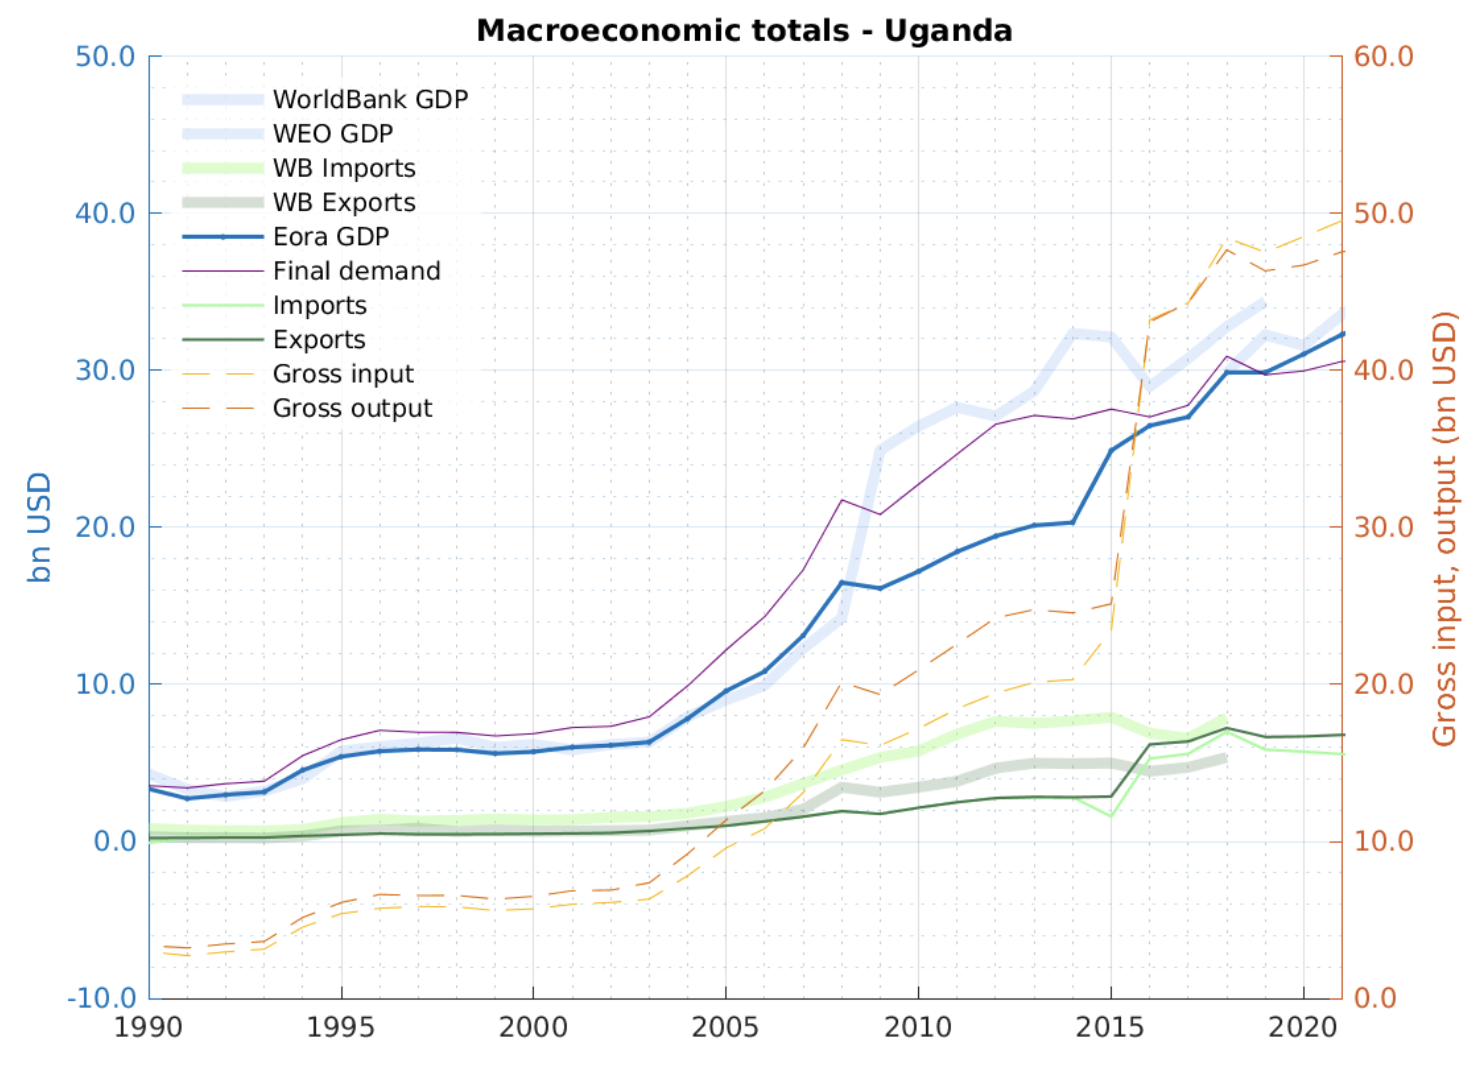
\includegraphics[width=0.5\textwidth, trim= {0 0 0 0}, clip]{"../Figures/DataQuality_UGA.png"} & 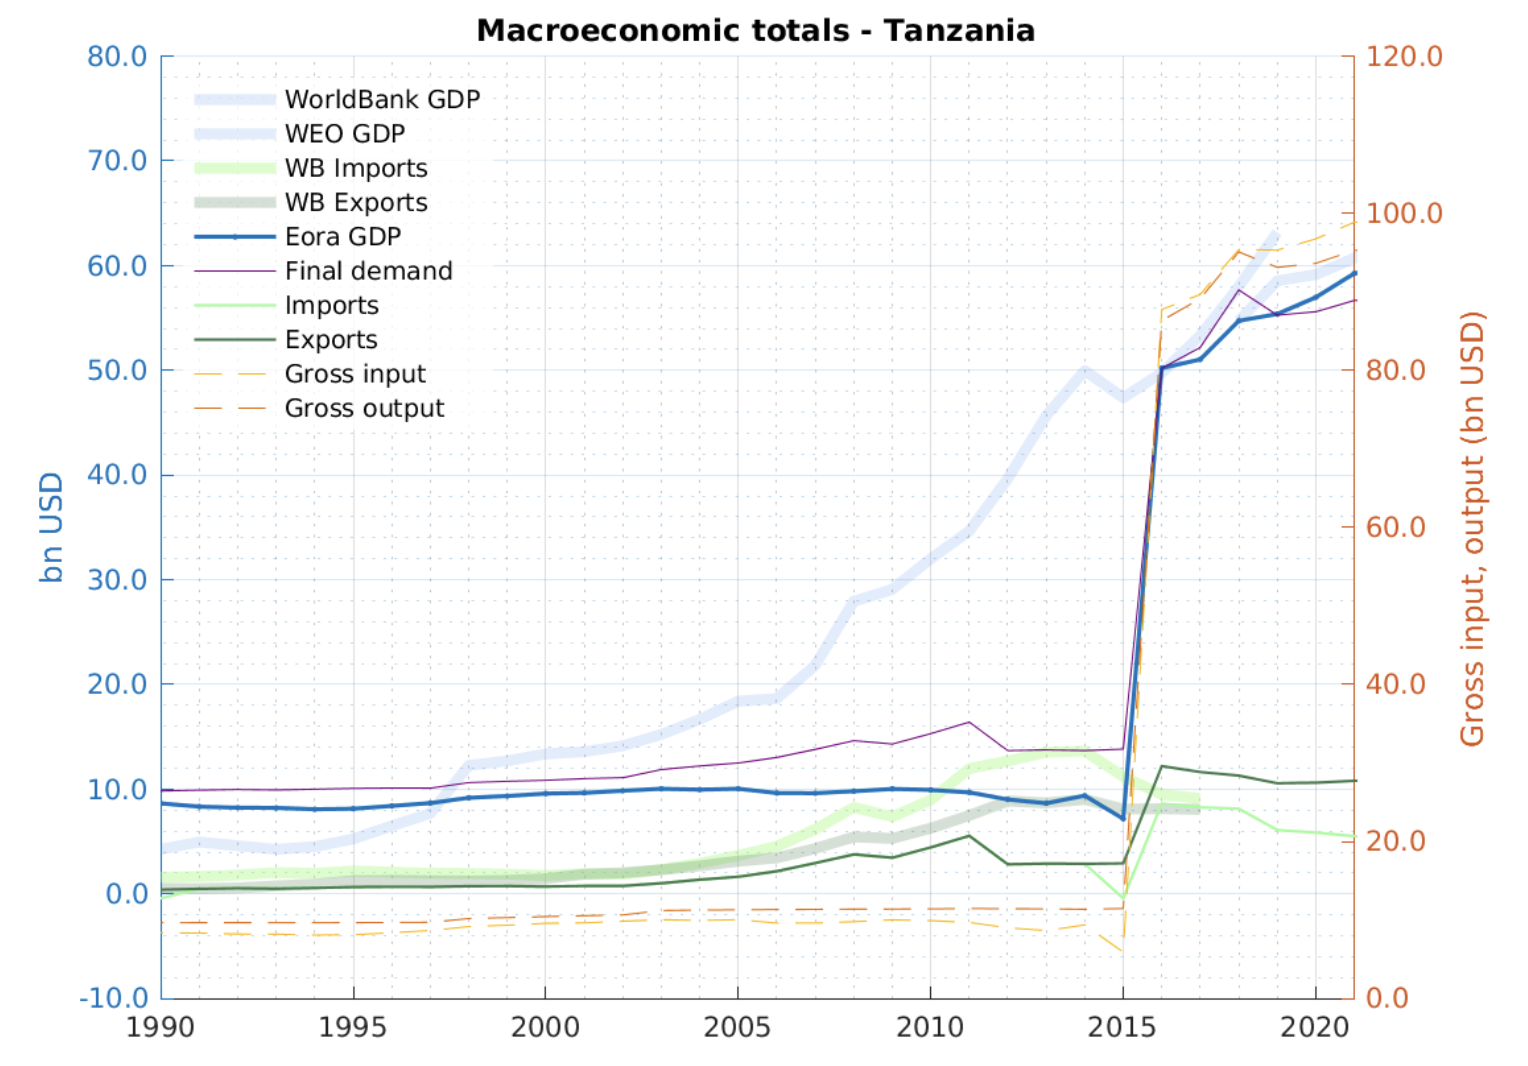
\includegraphics[width=0.52\textwidth, trim= {0 0 0 0}, clip]{"../Figures/DataQuality_TZA.png"} \\
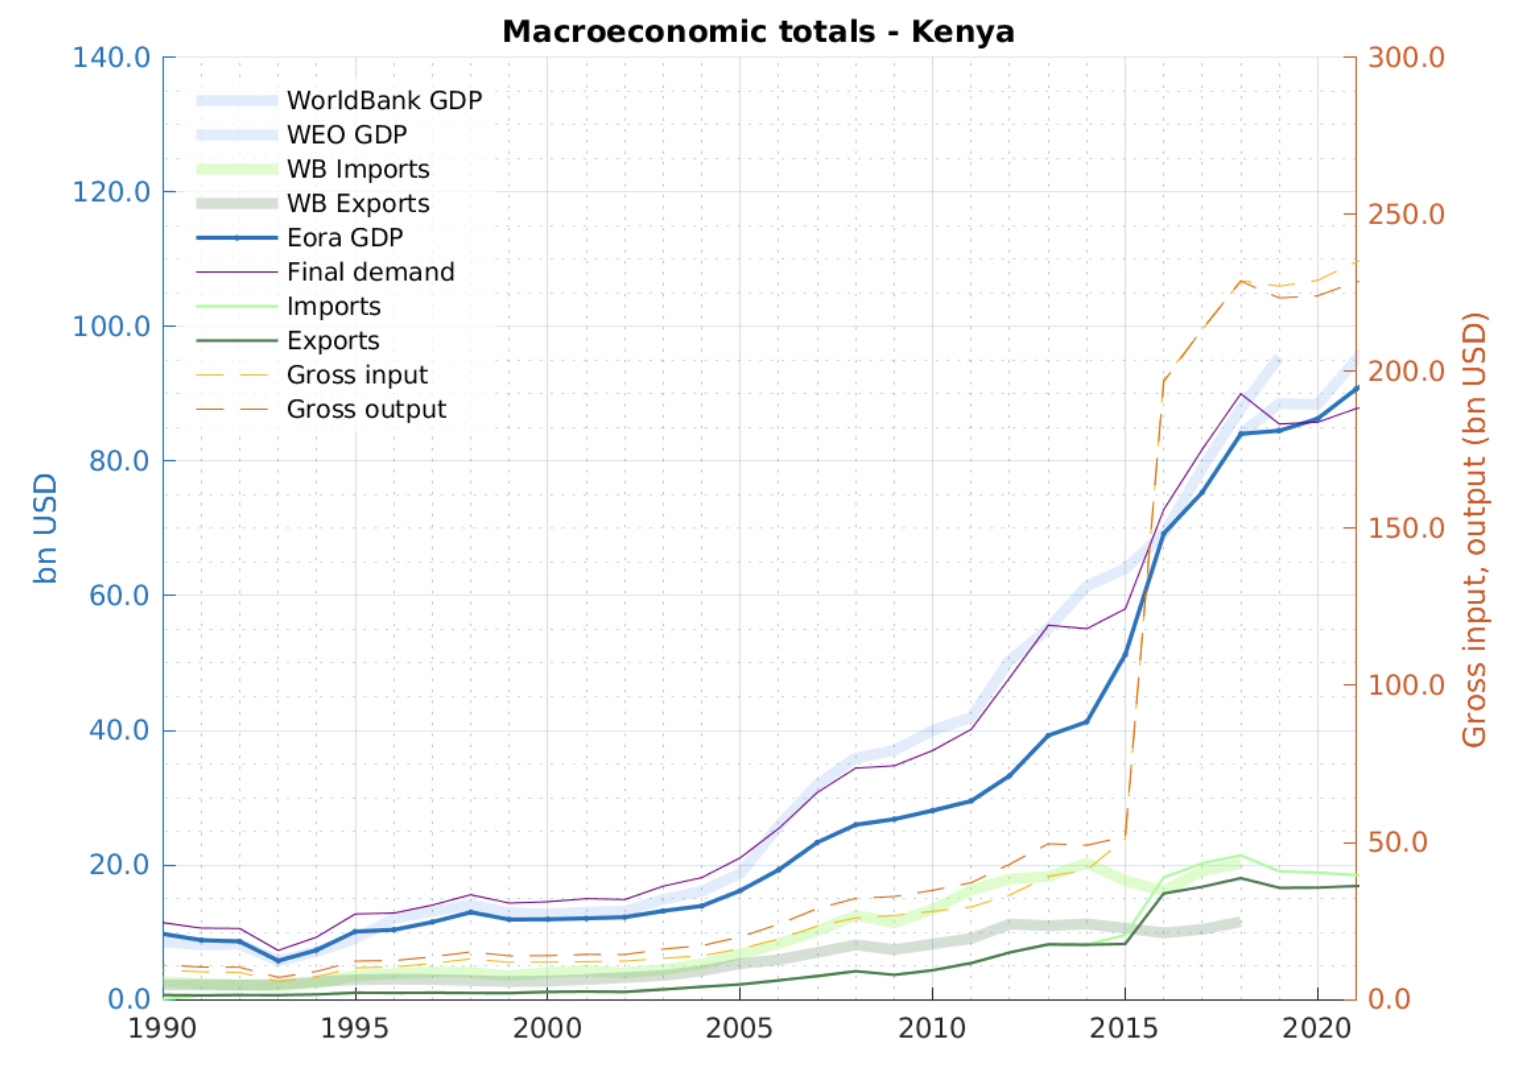
\includegraphics[width=0.5\textwidth, trim= {0 0 0 0}, clip]{"../Figures/DataQuality_KEN.png"} & 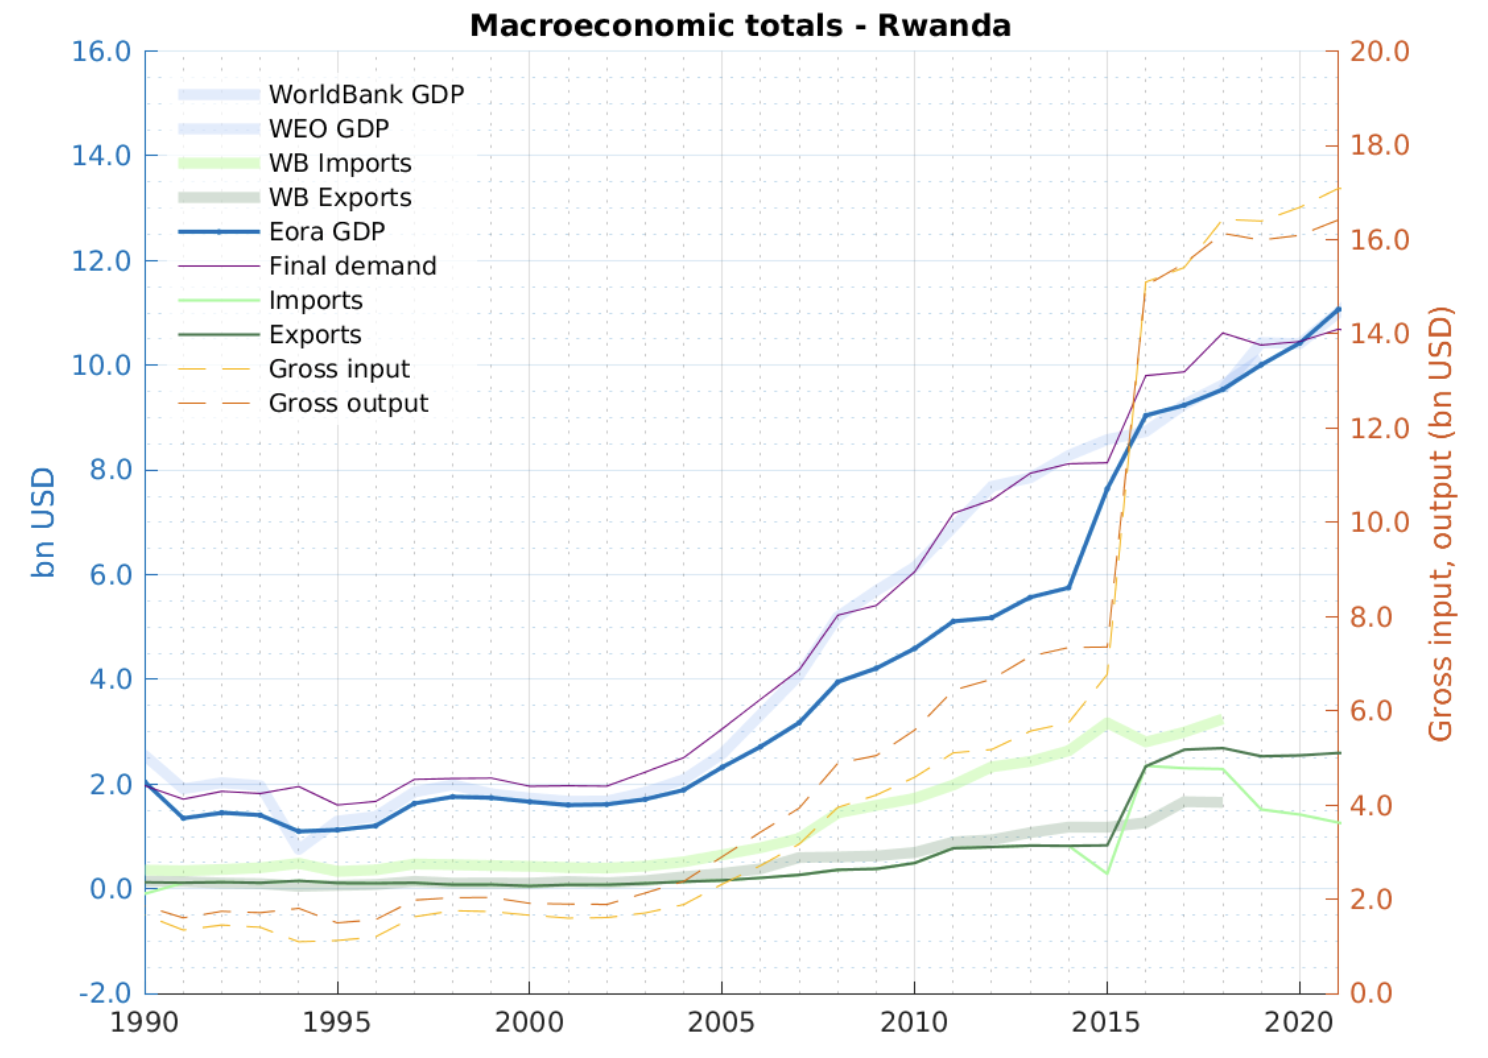
\includegraphics[width=0.5\textwidth, trim= {0 0 0 0}, clip]{"../Figures/DataQuality_RWA.png"} \\
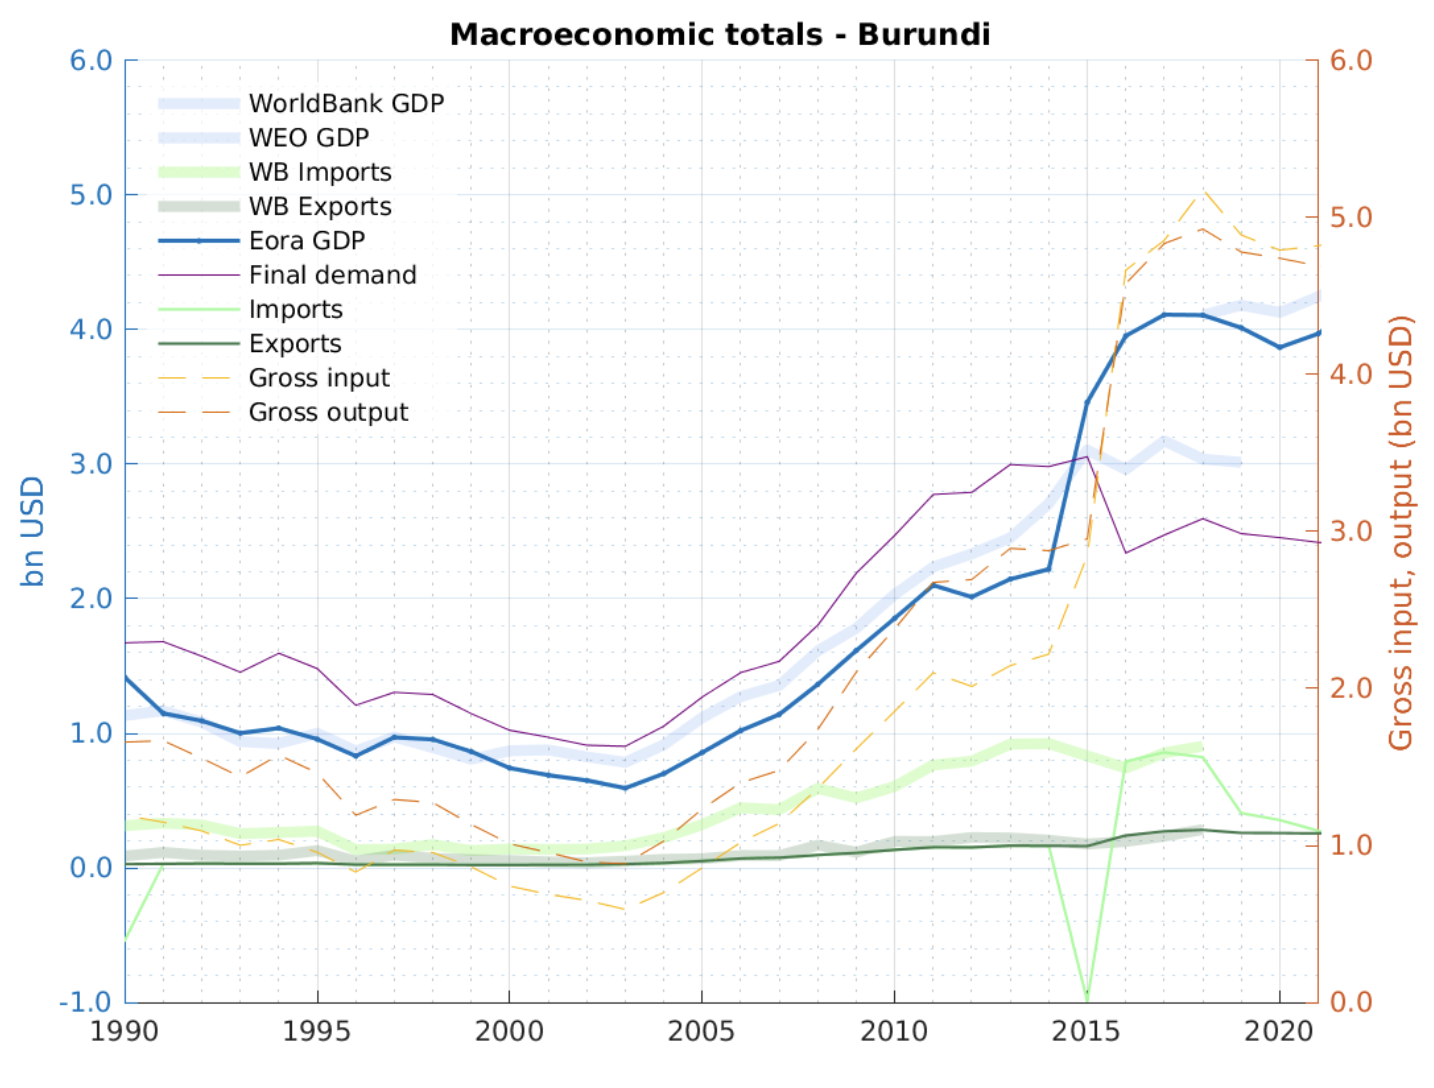
\includegraphics[width=0.5\textwidth, trim= {0 0 0 0}, clip]{"../Figures/DataQuality_BDI.png"} & 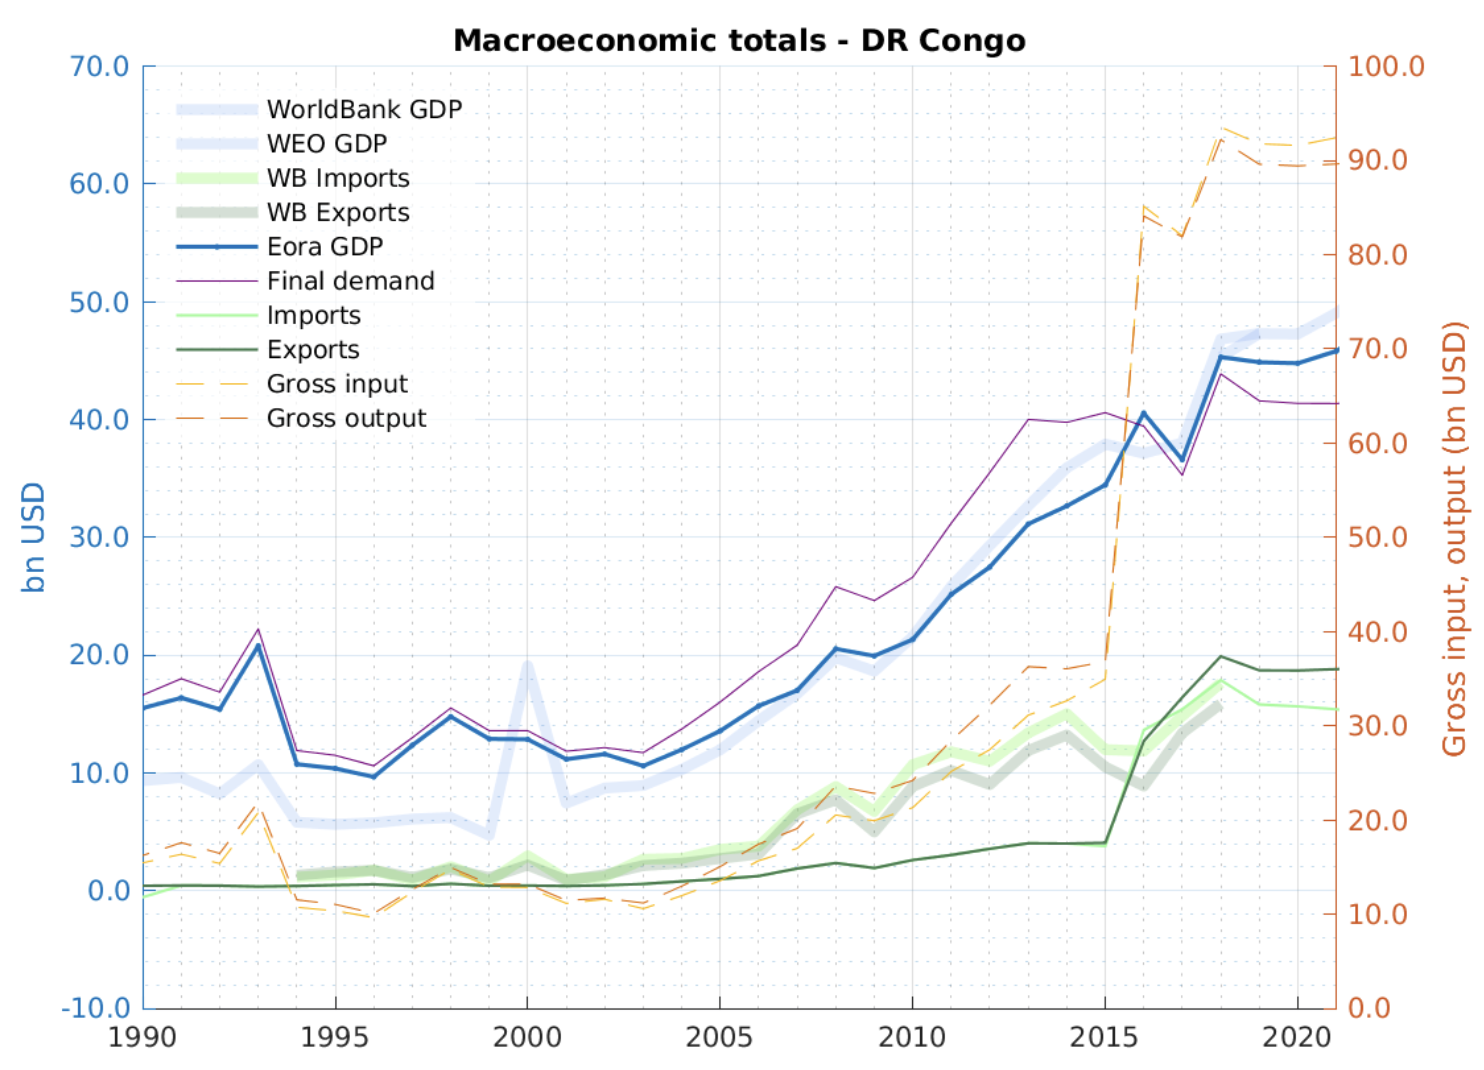
\includegraphics[width=0.5\textwidth, trim= {0 0 0 0}, clip]{"../Figures/DataQuality_COD.png"} \\
\end{tabular}
\end{figure}
\FloatBarrier




\subsection*{B. Additional Tables and Figures}
\setcounter{table}{0}
\renewcommand{\thetable}{B\arabic{table}}
\setcounter{figure}{0}
\renewcommand{\thefigure}{B\arabic{figure}}


\begin{figure}[h!] \vspace{-1mm}
\centering
\caption{\label{fig:MIG_SEC_EORA}\textsc{Average Trade Flows by Broad Sector, 2010-2015: EORA: USD Billions}}
\vspace{2mm}
\resizebox{\textwidth}{!}{
\begin{tabular}{ccc}
Agriculture \& Livestock & Foods \& Beverages & Manufactured Goods \\
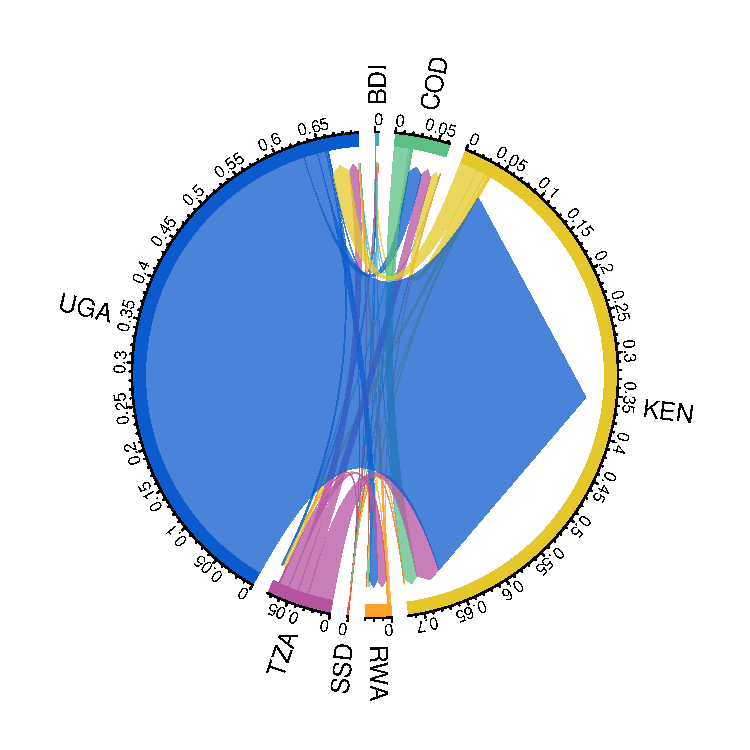
\includegraphics[width=0.4\textwidth, trim= {1.3cm 0.8cm 1.1cm 1cm}, clip]{"../Figures/REV/EORA_MIG_AGR_2010_19.pdf"} & 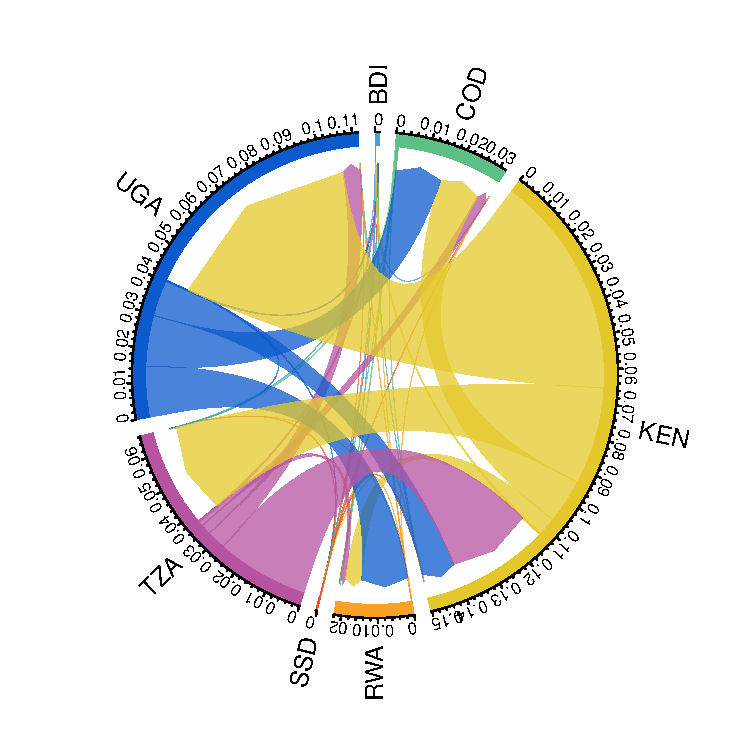
\includegraphics[width=0.4\textwidth, trim= {1.3cm 0.8cm 1.1cm 1cm}, clip]{"../Figures/REV/EORA_MIG_FBE_2010_19.pdf"} &
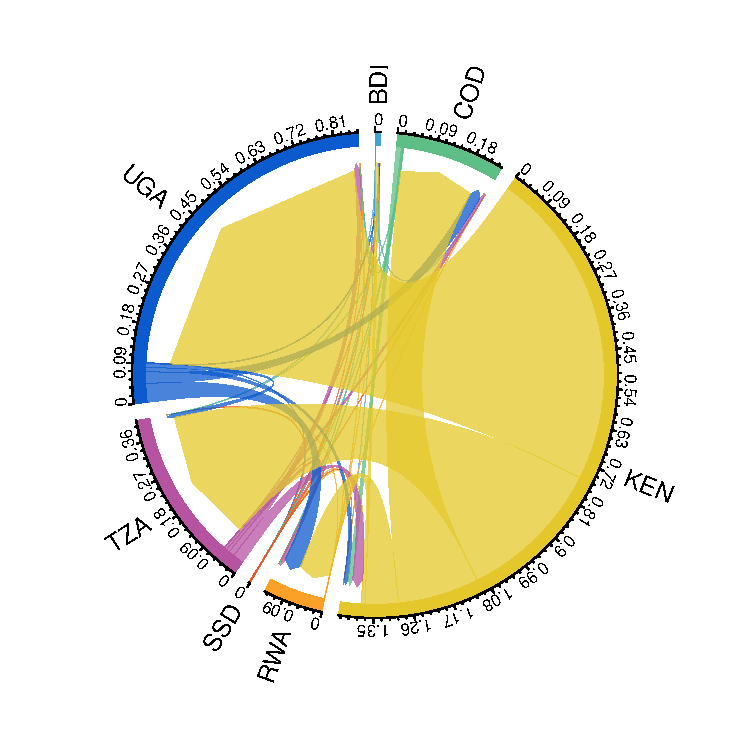
\includegraphics[width=0.4\textwidth, trim= {1.3cm 0.8cm 1.1cm 1cm}, clip]{"../Figures/REV/EORA_MIG_MAN_2010_19.pdf"} \\
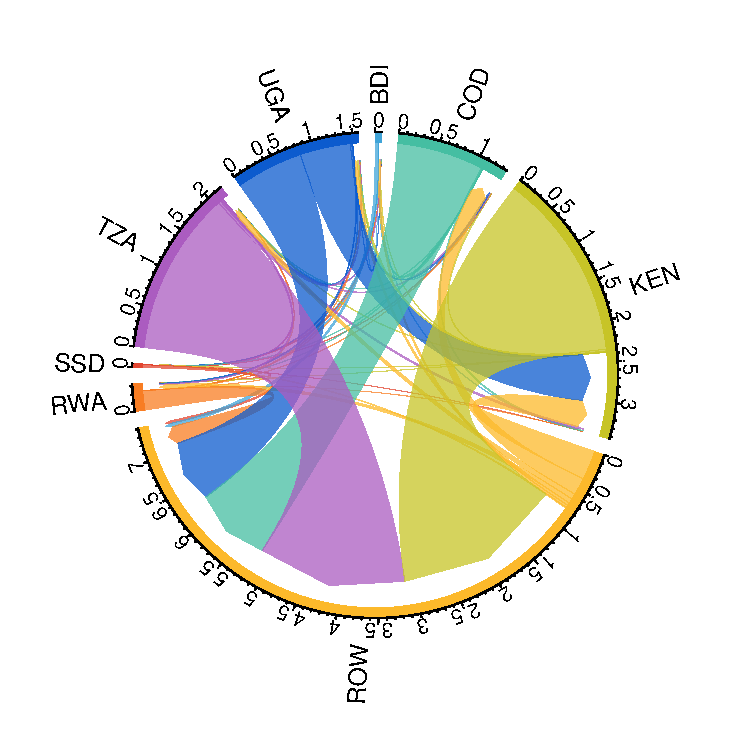
\includegraphics[width=0.4\textwidth, trim= {1.3cm 0.8cm 1.1cm 1cm}, clip]{"../Figures/REV/EORA_MIG_AGR_2010_19_ROW.pdf"} & 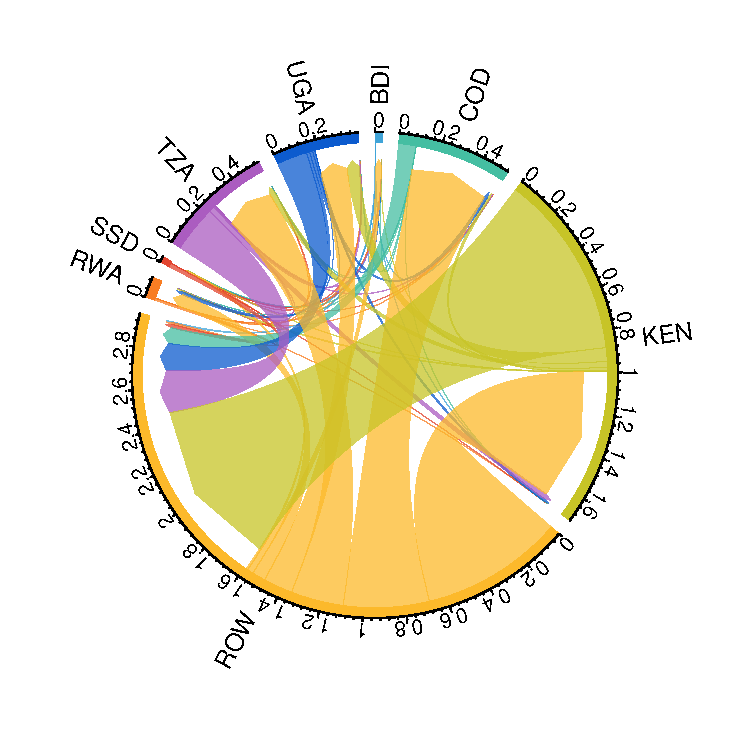
\includegraphics[width=0.4\textwidth, trim= {1.3cm 0.8cm 1.1cm 1cm}, clip]{"../Figures/REV/EORA_MIG_FBE_2010_19_ROW.pdf"} &
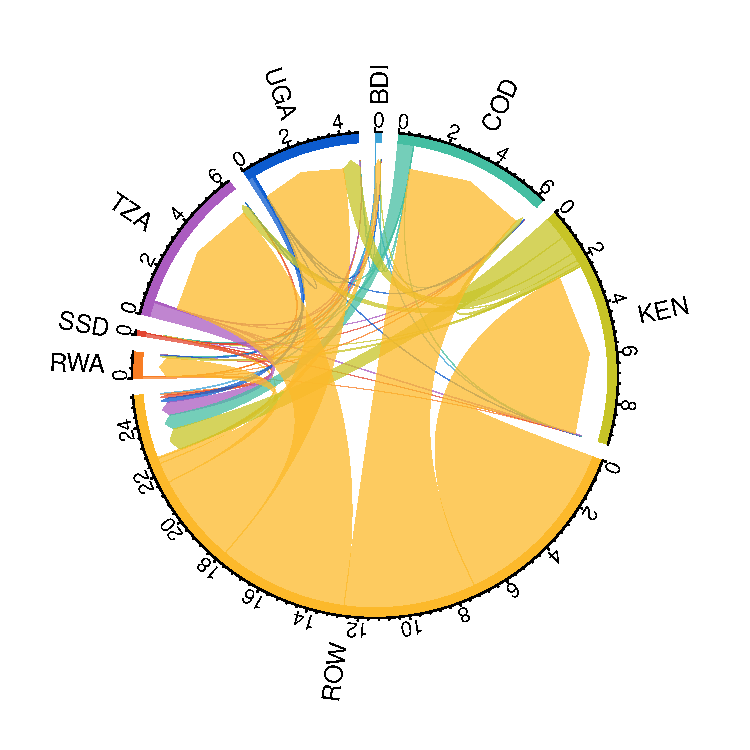
\includegraphics[width=0.4\textwidth, trim= {1.3cm 0.8cm 1.1cm 1cm}, clip]{"../Figures/REV/EORA_MIG_MAN_2010_19_ROW.pdf"} \\
\end{tabular}
}
\end{figure}
\FloatBarrier


\begin{figure}[h!] \vspace{-1mm}
\centering
\caption{\label{fig:MIG_SEC_EM}\textsc{Average Trade Flows by Broad Sector, 2010-2015: EMERGING: USD Billions}}
\vspace{2mm}
\resizebox{\textwidth}{!}{
\begin{tabular}{ccc}
Agriculture \& Livestock & Foods \& Beverages & Manufactured Goods \\
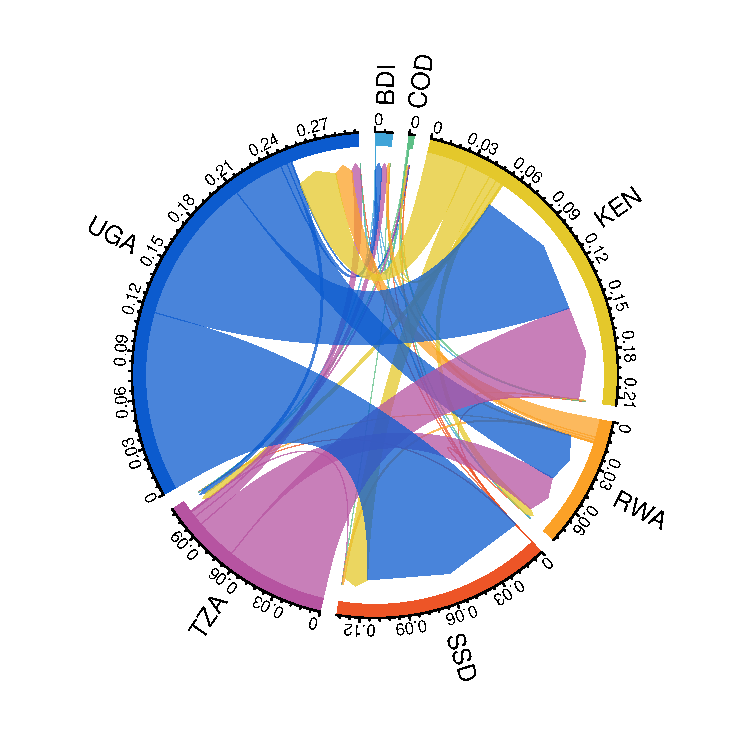
\includegraphics[width=0.4\textwidth, trim= {1.3cm 0.8cm 1.1cm 1cm}, clip]{"../Figures/REV/EM_MIG_AGR_2010_19.pdf"} & 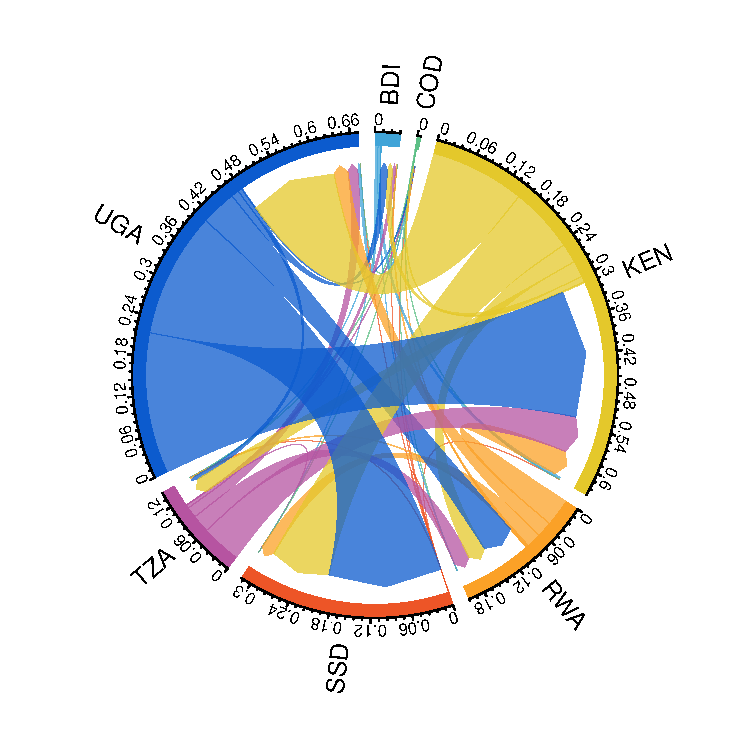
\includegraphics[width=0.4\textwidth, trim= {1.3cm 0.8cm 1.1cm 1cm}, clip]{"../Figures/REV/EM_MIG_FBE_2010_19.pdf"} &
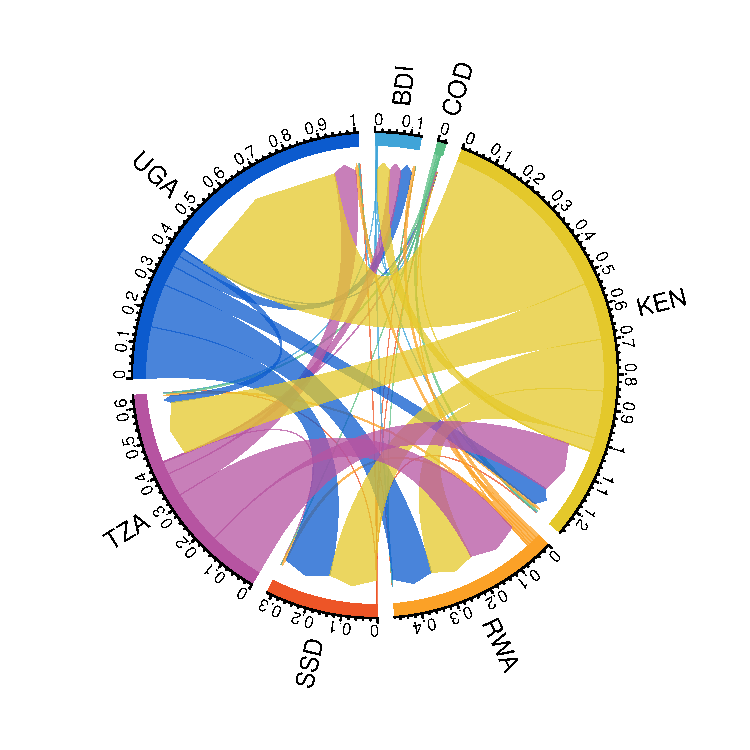
\includegraphics[width=0.4\textwidth, trim= {1.3cm 0.8cm 1.1cm 1cm}, clip]{"../Figures/REV/EM_MIG_MAN_2010_19.pdf"} \\
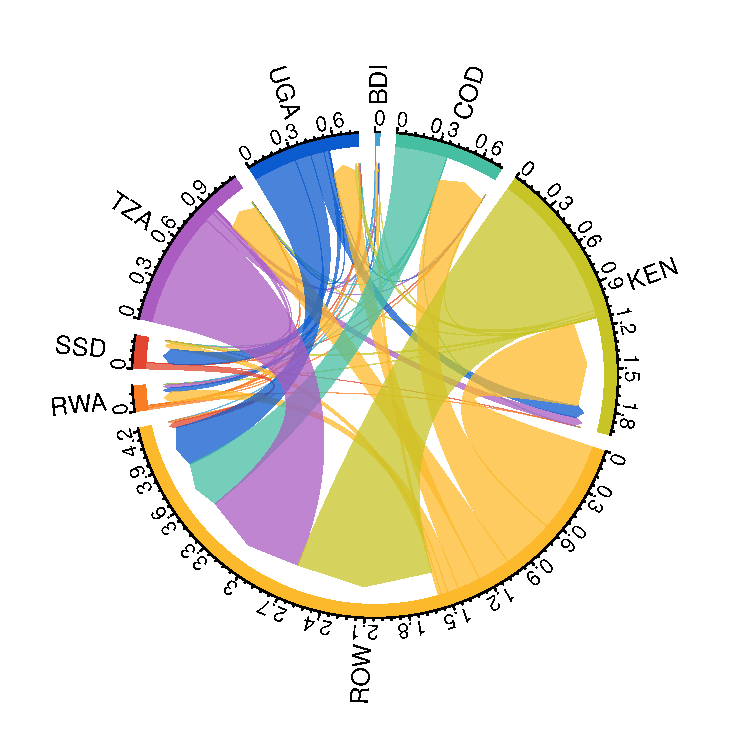
\includegraphics[width=0.4\textwidth, trim= {1.3cm 0.8cm 1.1cm 1cm}, clip]{"../Figures/REV/EM_MIG_AGR_2010_19_ROW.pdf"} & \includegraphics[width=0.4\textwidth, trim= {1.3cm 0.8cm 1.1cm 1cm}, clip]{"../Figures/REV/EM_MIG_FBE_2010_19_ROW.pdf"} &
\includegraphics[width=0.4\textwidth, trim= {1.3cm 0.8cm 1.1cm 1cm}, clip]{"../Figures/REV/EM_MIG_MAN_2010_19_ROW.pdf"} \\
\end{tabular}
}
\end{figure}
\FloatBarrier


\begin{table}[ht]
\centering
  \caption{\label{tab:weaclfl}\textsc{Largest 50 Intermediate EAC Trade Flows: EMERGING 2015-19 Average}} 
  \small{\textit{Millions of Current USD at Basic Prices}}
\begin{tabular}{rllrllr}
  \toprule
 & \multicolumn{3}{c}{Overall} & \multicolumn{3}{c}{Inner-EAC} \\
 & From & To & Value & From & To & Value \\ 
  \midrule
  2 & UGA.PCM & MEA.MIN & 254.72 & KEN.PCM & UGA.CON & 65.28 \\ 
  3 & MEA.PCM & KEN.FBE & 245.28 & KEN.PCM & RWA.AFF & 41.38 \\ 
  4 & SAS.PCM & TZA.TRA & 244.89 & KEN.PCM & UGA.FBE & 40.42 \\ 
  5 & SAS.PCM & KEN.FBE & 233.83 & UGA.FBE & KEN.TRA & 40.12 \\ 
  6 & CHN.TEX & TZA.TEX & 222.33 & UGA.FBE & KEN.FBE & 38.88 \\ 
  7 & CHN.TEX & KEN.TEX & 213.58 & TZA.PCM & RWA.AFF & 38.36 \\ 
  8 & CHN.PCM & KEN.PCM & 213.41 & UGA.PCM & RWA.AFF & 31.44 \\ 
  9 & CHN.ELM & TZA.ELM & 211.46 & KEN.MPR & UGA.CON & 31.15 \\ 
  10 & CHN.TEX & KEN.TRA & 211.10 & TZA.AFF & KEN.FBE & 30.07 \\ 
  11 & KEN.TRA & EUU.TRA & 207.65 & KEN.FBE & UGA.FBE & 29.40 \\ 
  12 & TZA.PCM & ECA.PCM & 196.53 & KEN.PCM & UGA.AFF & 29.18 \\ 
  13 & KEN.FBE & SAS.FBE & 196.09 & UGA.AFF & KEN.FBE & 28.80 \\ 
  14 & KEN.AFF & EUU.FBE & 191.72 & KEN.PCM & TZA.PCM & 27.12 \\ 
  15 & MEA.PCM & TZA.TRA & 191.05 & KEN.MPR & UGA.MPR & 22.62 \\ 
  16 & CHN.MPR & KEN.EGW & 186.79 & RWA.FBE & KEN.FBE & 21.90 \\ 
  17 & UGA.PCM & MEA.CON & 180.61 & TZA.TEX & KEN.TEX & 19.46 \\ 
  18 & CHN.TEX & KEN.WAP & 175.45 & RWA.FBE & KEN.TRA & 17.37 \\ 
  19 & SAS.PCM & KEN.PCM & 172.61 & UGA.EGW & KEN.CON & 17.14 \\ 
  20 & TZA.AFF & SAS.AFF & 163.76 & UGA.PCM & RWA.TRA & 16.29 \\ 
  21 & KEN.AFF & EUU.AFF & 160.71 & KEN.FBE & UGA.SMH & 14.99 \\ 
  22 & CHN.PCM & KEN.FBE & 158.19 & UGA.AFF & KEN.AFF & 14.28 \\ 
  23 & SAS.PCM & KEN.EGW & 156.87 & KEN.MPR & UGA.PTE & 13.76 \\ 
  24 & TZA.PCM & SSA.MPR & 155.21 & TZA.WAP & KEN.WAP & 13.70 \\ 
  25 & MEA.PCM & KEN.PCM & 142.64 & TZA.FBE & KEN.TEX & 13.64 \\ 
  26 & MEA.PCM & KEN.EGW & 142.53 & KEN.PCM & TZA.FBE & 13.10 \\ 
  27 & CHN.PCM & TZA.CON & 136.05 & UGA.FBE & RWA.TRA & 13.07 \\ 
  28 & CHN.PCM & TZA.PCM & 135.90 & KEN.AFF & UGA.FBE & 12.36 \\ 
  29 & TZA.TRA & EUU.TRA & 131.02 & UGA.FBE & KEN.TEX & 12.33 \\ 
  30 & KEN.FBE & SAS.PCM & 129.12 & KEN.PCM & UGA.TRA & 12.22 \\ 
  31 & UGA.PCM & MEA.PCM & 129.11 & KEN.PCM & UGA.EGW & 11.55 \\ 
  32 & MEA.PCM & KEN.CON & 128.95 & UGA.WAP & KEN.WAP & 11.23 \\ 
  33 & EUU.PCM & KEN.PCM & 114.90 & KEN.TEX & UGA.TEX & 10.58 \\ 
  34 & CHN.PCM & KEN.AFF & 114.73 & TZA.FBE & KEN.FBE & 10.45 \\ 
  35 & SAS.PCM & KEN.AFF & 113.57 & TZA.FBE & KEN.PCM & 10.21 \\ 
  36 & EUU.PCM & KEN.FBE & 113.21 & TZA.WAP & KEN.FBE & 9.72 \\ 
  37 & CHN.ELM & TZA.CON & 113.02 & UGA.FBE & KEN.PCM & 8.79 \\ 
  38 & CHN.ELM & UGA.EGW & 112.73 & UGA.WAP & KEN.FBE & 8.42 \\ 
  39 & MEA.PCM & TZA.CON & 106.08 & KEN.PCM & RWA.FBE & 8.40 \\ 
  40 & KEN.FBE & MEA.FBE & 104.53 & TZA.TEX & KEN.TRA & 8.00 \\ 
  41 & CHN.MAN & KEN.MAN & 104.29 & KEN.PCM & BDI.AFF & 8.00 \\ 
  42 & UGA.FBE & EUU.FBE & 102.62 & KEN.FBE & UGA.TRA & 7.66 \\ 
  43 & TZA.AFF & ASE.AFF & 102.24 & TZA.FBE & KEN.TRA & 7.18 \\ 
  44 & CHN.ELM & KEN.CON & 100.89 & TZA.AFF & KEN.AFF & 6.96 \\ 
  45 & CHN.MPR & TZA.ELM & 98.29 & KEN.PCM & TZA.CON & 6.93 \\ 
  46 & KEN.FBE & EUU.FBE & 96.18 & KEN.PCM & TZA.TRA & 6.83 \\ 
  47 & TZA.PCM & SSA.PCM & 95.74 & TZA.PCM & BDI.AFF & 6.80 \\ 
  48 & CHN.ELM & KEN.FBE & 94.59 & KEN.FBE & UGA.PTE & 6.49 \\ 
  49 & SAS.PCM & KEN.CON & 93.59 & KEN.PCM & TZA.AFF & 6.48 \\ 
  50 & TZA.TRA & SAS.TRA & 91.13 & KEN.WAP & RWA.CON & 6.43 \\ 
   \bottomrule
\end{tabular}
\end{table}
\FloatBarrier


\begin{figure}[h!] 
\centering
\caption{\label{fig:KWW}\textsc{Refined Koopman Wang Wei Decomposition of Gross Exports}}
\includegraphics[width=1\textwidth, trim= {0 0 0 0}, clip]{"../Figures/REV/KWW_DEC_NEW.png"} \raggedleft
\scriptsize
\emph{Source:} \citet{antras2022global}
\end{figure}
\FloatBarrier

\vspace{1cm}

\begin{figure}[h!]
\centering
\caption{\label{fig:KWW_fill_ts}\textsc{KWW Decomposition of Gross Exports}}
\includegraphics[width=1\textwidth]{"../Figures/REV/KWW_DEC_NEW.pdf"} \end{figure}
\FloatBarrier


\newpage


\begin{table}[ht]
\centering
\caption{\label{tab:NRCA} (N)RCA Estimates from Figure \ref{fig:NRCA}}
\vspace{2mm}
\resizebox{\textwidth}{!}{
\begin{tabular}{lllrrrrrrrrrrrrrrrrr}
  \toprule
Country & Source & Flow & AFF & MIN & FBE & TEX & WAP & PCM & MPR & ELM & TEQ & MAN & EGW & CON & SMH & TRA & PTE & FIB & PAO \\ 
  \midrule
UGA & WDR\_EORA & GX & 16.07 & 0.14 & 2.49 & 0.24 & 0.29 & 0.18 & 0.39 & 0.18 & 0.28 & 0.95 & 0.93 & 4.57 & 2.33 & 2.04 & 2.76 & 0.02 & 1.09 \\ 
  TZA & WDR\_EORA & GX & 10.48 & 1.48 & 2.42 & 1.63 & 0.57 & 0.21 & 0.20 & 0.12 & 0.29 & 4.58 & 3.99 & 2.03 & 1.15 & 1.06 & 1.43 & 1.02 & 0.58 \\ 
  KEN & WDR\_EORA & GX & 11.57 & 1.09 & 2.95 & 0.94 & 0.94 & 0.73 & 0.44 & 0.26 & 0.08 & 1.04 & 1.61 & 1.11 & 1.41 & 1.70 & 1.73 & 0.44 & 0.19 \\ 
  RWA & WDR\_EORA & GX & 4.40 & 4.49 & 0.29 & 0.29 & 0.35 & 0.16 & 0.32 & 0.11 & 0.10 & 0.67 & 4.86 & 9.81 & 4.05 & 1.69 & 5.12 & 0.12 & 2.55 \\ 
  BDI & WDR\_EORA & GX & 6.83 & 0.32 & 0.31 & 0.38 & 0.20 & 0.13 & 0.24 & 0.07 & 0.25 & 1.18 & 4.23 & 12.99 & 5.53 & 1.82 & 6.10 & 0.10 & 3.50 \\ 
  EAC5 & WDR\_EORA & GX & 11.54 & 1.10 & 2.68 & 0.96 & 0.77 & 0.55 & 0.38 & 0.22 & 0.14 & 1.64 & 2.09 & 2.17 & 1.64 & 1.63 & 2.00 & 0.48 & 0.50 \\ \midrule
  UGA & EORA & GX & 17.33 & 0.11 & 2.83 & 0.22 & 0.36 & 0.19 & 0.39 & 0.16 & 0.35 & 0.79 & 1.25 & 3.98 & 2.05 & 1.81 & 2.69 & 0.02 & 1.35 \\ 
  TZA & EORA & GX & 11.30 & 1.08 & 2.69 & 1.56 & 0.71 & 0.22 & 0.20 & 0.10 & 0.38 & 3.97 & 4.98 & 1.72 & 0.98 & 0.93 & 1.34 & 1.00 & 0.67 \\ 
  KEN & EORA & GX & 11.95 & 0.79 & 3.41 & 0.89 & 1.20 & 0.77 & 0.44 & 0.23 & 0.11 & 0.92 & 2.20 & 0.95 & 1.24 & 1.56 & 1.73 & 0.44 & 0.25 \\ 
  RWA & EORA & GX & 4.82 & 3.38 & 0.34 & 0.28 & 0.45 & 0.17 & 0.32 & 0.10 & 0.14 & 0.58 & 6.55 & 8.74 & 3.56 & 1.50 & 5.07 & 0.12 & 3.23 \\ 
  BDI & EORA & GX & 7.43 & 0.24 & 0.36 & 0.35 & 0.26 & 0.13 & 0.25 & 0.07 & 0.34 & 0.98 & 5.49 & 11.58 & 4.86 & 1.62 & 6.05 & 0.10 & 4.40 \\ 
  EAC5 & EORA & GX & 12.28 & 0.83 & 3.07 & 0.90 & 0.98 & 0.58 & 0.38 & 0.20 & 0.19 & 1.39 & 2.92 & 1.91 & 1.43 & 1.45 & 1.94 & 0.47 & 0.65 \\ \midrule
  UGA & EMERGING & GX & 4.76 & 0.00 & 7.16 & 0.52 & 0.70 & 0.82 & 0.46 & 0.03 & 0.05 & 0.14 & 7.29 & 0.19 & 4.42 & 1.92 & 0.03 & 0.16 & 0.12 \\ 
  TZA & EMERGING & GX & 4.93 & 0.01 & 2.46 & 0.55 & 0.64 & 1.38 & 0.58 & 0.04 & 0.04 & 0.12 & 0.00 & 1.61 & 3.04 & 3.41 & 0.27 & 0.02 & 0.06 \\ 
  KEN & EMERGING & GX & 4.16 & 0.01 & 5.98 & 1.01 & 0.94 & 0.55 & 0.47 & 0.06 & 0.10 & 0.33 & 1.17 & 0.00 & 2.17 & 3.28 & 0.29 & 0.13 & 6.78 \\ 
  RWA & EMERGING & GX & 0.74 & 0.00 & 5.11 & 0.24 & 0.07 & 1.41 & 0.17 & 0.05 & 0.06 & 0.10 & 0.69 & 0.51 & 5.67 & 2.00 & 0.02 & 0.01 & 2.26 \\ 
  BDI & EMERGING & GX & 0.16 & 0.00 & 10.83 & 0.31 & 0.06 & 0.95 & 0.22 & 0.04 & 0.08 & 0.07 & 0.00 & 0.01 & 0.02 & 1.30 & 0.12 & 0.01 & 24.16 \\ 
  EAC5 & EMERGING & GX & 4.12 & 0.01 & 5.12 & 0.70 & 0.77 & 0.90 & 0.49 & 0.06 & 0.08 & 0.21 & 2.09 & 0.61 & 3.08 & 2.90 & 0.21 & 0.09 & 3.16 \\ \midrule
  UGA & BACI & GX & 5.03 & 0.08 & 7.60 & 0.88 & 0.73 & 0.68 & 0.80 & 0.18 & 0.20 & 0.24 &  &  &  &  &  &  &  \\ 
  TZA & BACI & GX & 5.08 & 0.23 & 2.85 & 0.93 & 0.60 & 2.42 & 0.58 & 0.13 & 0.08 & 0.16 &  &  &  &  &  &  &  \\ 
  KEN & BACI & GX & 5.74 & 0.45 & 6.61 & 1.63 & 0.89 & 0.77 & 0.59 & 0.17 & 0.12 & 0.40 &  &  &  &  &  &  &  \\ 
  RWA & BACI & GX & 1.27 & 0.65 & 5.02 & 0.51 & 0.18 & 2.32 & 0.26 & 0.07 & 0.11 & 0.18 &  &  &  &  &  &  &  \\ 
  BDI & BACI & GX & 0.25 & 0.02 & 5.53 & 0.42 & 0.06 & 2.84 & 0.30 & 0.07 & 0.09 & 0.11 &  &  &  &  &  &  &  \\ 
  EAC5 & BACI & GX & 5.21 & 0.32 & 5.16 & 1.19 & 0.73 & 1.55 & 0.58 & 0.15 & 0.15 & 0.28 &  &  &  &  &  &  &  \\ \midrule
  UGA & WDR\_EORA & VAX & 13.87 & 0.11 & 2.24 & 0.20 & 0.25 & 0.16 & 0.33 & 0.15 & 0.24 & 0.82 & 0.78 & 4.02 & 1.94 & 1.79 & 2.37 & 0.02 & 3.42 \\ 
  TZA & WDR\_EORA & VAX & 10.87 & 1.23 & 2.07 & 1.31 & 0.42 & 0.16 & 0.13 & 0.07 & 0.15 & 3.15 & 3.76 & 1.75 & 1.01 & 0.91 & 1.39 & 1.04 & 1.76 \\ 
  KEN & WDR\_EORA & VAX & 10.62 & 0.84 & 2.63 & 0.91 & 0.84 & 0.72 & 0.29 & 0.19 & 0.06 & 0.98 & 1.52 & 0.86 & 1.22 & 1.42 & 1.53 & 0.38 & 0.64 \\ 
  RWA & WDR\_EORA & VAX & 4.55 & 3.74 & 0.31 & 0.24 & 0.35 & 0.17 & 0.30 & 0.11 & 0.09 & 0.27 & 4.23 & 10.26 & 3.49 & 1.70 & 5.07 & 0.11 & 4.19 \\ 
  BDI & WDR\_EORA & VAX & 6.36 & 0.19 & 0.31 & 0.30 & 0.20 & 0.13 & 0.23 & 0.08 & 0.26 & 0.82 & 3.41 & 12.58 & 4.41 & 1.72 & 5.43 & 0.09 & 9.87 \\ 
  EAC5 & WDR\_EORA & VAX & 10.80 & 0.86 & 2.38 & 0.85 & 0.68 & 0.54 & 0.27 & 0.16 & 0.10 & 1.24 & 1.87 & 1.91 & 1.42 & 1.41 & 1.80 & 0.42 & 1.44 \\ \midrule
  UGA & EORA & VAX & 16.59 & 0.10 & 2.57 & 0.19 & 0.32 & 0.16 & 0.34 & 0.14 & 0.28 & 0.71 & 1.19 & 3.72 & 1.92 & 1.73 & 2.55 & 0.02 & 1.57 \\ 
  TZA & EORA & VAX & 13.12 & 1.06 & 2.19 & 1.24 & 0.52 & 0.15 & 0.12 & 0.06 & 0.16 & 2.74 & 5.25 & 1.53 & 0.95 & 0.85 & 1.40 & 1.12 & 0.75 \\ 
  KEN & EORA & VAX & 12.20 & 0.72 & 3.07 & 0.89 & 1.09 & 0.75 & 0.30 & 0.17 & 0.07 & 0.90 & 2.32 & 0.80 & 1.21 & 1.41 & 1.69 & 0.43 & 0.32 \\ 
  RWA & EORA & VAX & 5.37 & 3.29 & 0.37 & 0.23 & 0.46 & 0.18 & 0.30 & 0.10 & 0.12 & 0.26 & 6.42 & 9.69 & 3.43 & 1.65 & 5.46 & 0.13 & 2.10 \\ 
  BDI & EORA & VAX & 7.67 & 0.17 & 0.37 & 0.29 & 0.26 & 0.14 & 0.25 & 0.08 & 0.32 & 0.75 & 4.96 & 12.92 & 4.37 & 1.68 & 5.95 & 0.11 & 4.75 \\ 
  EAC5 & EORA & VAX & 12.68 & 0.76 & 2.76 & 0.83 & 0.88 & 0.56 & 0.28 & 0.14 & 0.12 & 1.10 & 2.97 & 1.78 & 1.39 & 1.35 & 1.93 & 0.47 & 0.72 \\ \midrule
  UGA & EMERGING & VAX & 4.67 & 0.00 & 6.15 & 0.42 & 0.65 & 0.79 & 0.40 & 0.03 & 0.05 & 0.12 & 5.87 & 0.18 & 4.36 & 1.92 & 0.02 & 0.16 & 0.11 \\ 
  TZA & EMERGING & VAX & 5.08 & 0.01 & 2.53 & 0.55 & 0.58 & 1.43 & 0.51 & 0.03 & 0.04 & 0.10 & 0.00 & 1.58 & 2.83 & 3.02 & 0.23 & 0.02 & 0.06 \\ 
  KEN & EMERGING & VAX & 4.05 & 0.01 & 5.79 & 0.84 & 0.60 & 0.52 & 0.47 & 0.05 & 0.07 & 0.26 & 0.99 & 0.00 & 2.00 & 3.13 & 0.27 & 0.13 & 6.02 \\ 
  RWA & EMERGING & VAX & 0.77 & 0.00 & 4.50 & 0.26 & 0.08 & 1.56 & 0.18 & 0.06 & 0.08 & 0.11 & 0.79 & 0.52 & 4.64 & 2.06 & 0.02 & 0.01 & 2.30 \\ 
  BDI & EMERGING & VAX & 0.16 & 0.00 & 9.67 & 0.34 & 0.06 & 0.69 & 0.18 & 0.04 & 0.07 & 0.09 & 0.00 & 0.01 & 0.02 & 1.47 & 0.13 & 0.01 & 26.19 \\ 
  EAC5 & EMERGING & VAX & 4.17 & 0.01 & 5.01 & 0.61 & 0.58 & 0.89 & 0.43 & 0.05 & 0.08 & 0.18 & 1.73 & 0.58 & 2.85 & 2.77 & 0.19 & 0.09 & 2.91 \\ 
   \bottomrule
\end{tabular}
}
\end{table}


\begin{table}[ht]
\centering
\caption{\label{tab:NRCA_corr}\textsc{(New) Revealed Comparative Advantage: Correlations of 2010-19 Medians}}
\vspace{2mm}
\begin{tabular}{lrrrrrrr}
  \toprule
  & \multicolumn{2}{c}{WDR EORA} & \multicolumn{2}{c}{EORA} & \multicolumn{2}{c}{EMERGING} & BACI \\
 & GX & VAX & GX & VAX & GX & VAX & GX \\ 
  \midrule
  WDR\_EORA\_GX &    1   &  .962 &  .990 &  .987 &  .179 &  .186 &  .550 \\ 
  WDR\_EORA\_VAX &  .962 &    1   &  .960 &  .967 &  .341 &  .362 &  .563 \\ 
  EORA\_GX &  .990 &  .960 &    1   &  .995 &  .215 &  .223 &  .571 \\ 
  EORA\_VAX &  .987 &  .967 &  .995 &    1   &  .217 &  .227 &  .570 \\ 
  EMERGING\_GX &  .179 &  .341 &  .215 &  .217 &    1   &  .994 &  .925 \\ 
  EMERGING\_VAX &  .186 &  .362 &  .223 &  .227 &  .994 &    1   &  .934 \\ 
  BACI\_GX &  .550 &  .563 &  .571 &  .570 &  .925 &  .934 &    1   \\ 
   \bottomrule \\ [-0.9em]
\multicolumn{8}{l}{\parbox{0.7\textwidth}{\scriptsize
\textit{Notes:} WDR EORA is only available for 2010-15, EMERGING misses years 2011-14.}}
\end{tabular}
\end{table}


\begin{table}[ht]
\centering
\caption{\label{tab:EAC_NRCA} (N)RCA Estimates from Figure \ref{fig:EAC_NRCA}}
\vspace{2mm}
\resizebox{\textwidth}{!}{
\begin{tabular}{lllrrrrrrrrrrrrrrrrr}
  \toprule
Country & Source & Flow & AFF & MIN & FBE & TEX & WAP & PCM & MPR & ELM & TEQ & MAN & EGW & CON & SMH & TRA & PTE & FIB & PAO \\ 
  \midrule
 \multicolumn{10}{l}{Relative to the EAC} \\ \midrule
  UGA & WDR\_EORA & GX & 1.39 & 0.13 & 0.93 & 0.26 & 0.38 & 0.33 & 1.02 & 0.81 & 1.95 & 0.58 & 0.43 & 2.12 & 1.41 & 1.25 & 1.37 & 0.05 & 2.17 \\ 
  TZA & WDR\_EORA & GX & 0.91 & 1.32 & 0.91 & 1.71 & 0.74 & 0.38 & 0.52 & 0.54 & 2.04 & 2.80 & 1.90 & 0.93 & 0.70 & 0.65 & 0.71 & 2.12 & 1.16 \\ 
  KEN & WDR\_EORA & GX & 1.00 & 0.98 & 1.10 & 0.99 & 1.22 & 1.32 & 1.14 & 1.19 & 0.56 & 0.64 & 0.77 & 0.51 & 0.87 & 1.04 & 0.88 & 0.92 & 0.38 \\ 
  RWA & WDR\_EORA & GX & 0.39 & 4.06 & 0.11 & 0.30 & 0.45 & 0.29 & 0.84 & 0.50 & 0.69 & 0.40 & 2.35 & 4.57 & 2.47 & 1.04 & 2.56 & 0.24 & 5.20 \\ 
  BDI & WDR\_EORA & GX & 0.60 & 0.29 & 0.12 & 0.39 & 0.26 & 0.23 & 0.64 & 0.34 & 1.73 & 0.71 & 2.01 & 6.05 & 3.38 & 1.12 & 3.07 & 0.21 & 7.14 \\ \midrule
  UGA & EORA & GX & 1.34 & 0.13 & 0.91 & 0.26 & 0.39 & 0.32 & 1.03 & 0.80 & 1.88 & 0.57 & 0.45 & 2.06 & 1.40 & 1.24 & 1.36 & 0.05 & 2.10 \\ 
  TZA & EORA & GX & 0.92 & 1.25 & 0.87 & 1.68 & 0.72 & 0.37 & 0.50 & 0.52 & 2.02 & 2.76 & 1.83 & 0.90 & 0.68 & 0.64 & 0.69 & 2.12 & 1.11 \\ 
  KEN & EORA & GX & 0.99 & 1.00 & 1.12 & 0.99 & 1.23 & 1.33 & 1.15 & 1.20 & 0.58 & 0.64 & 0.79 & 0.54 & 0.88 & 1.05 & 0.89 & 0.94 & 0.40 \\ 
  RWA & EORA & GX & 0.40 & 3.96 & 0.11 & 0.31 & 0.46 & 0.30 & 0.86 & 0.50 & 0.72 & 0.41 & 2.24 & 4.48 & 2.46 & 1.01 & 2.55 & 0.24 & 5.02 \\ 
  BDI & EORA & GX & 0.59 & 0.28 & 0.12 & 0.40 & 0.27 & 0.23 & 0.65 & 0.34 & 1.78 & 0.73 & 1.94 & 6.26 & 3.42 & 1.09 & 3.03 & 0.22 & 6.88 \\ \midrule
  UGA & EMERGING & GX & 1.02 & 0.07 & 1.43 & 0.74 & 0.82 & 0.82 & 0.85 & 0.47 & 0.70 & 0.51 & 4.06 & 0.31 & 1.40 & 0.65 & 0.13 & 1.71 & 0.04 \\ 
  TZA & EMERGING & GX & 1.12 & 1.83 & 0.56 & 0.80 & 1.08 & 1.48 & 1.14 & 0.73 & 0.50 & 0.59 & 0.00 & 2.71 & 0.97 & 1.17 & 1.27 & 0.22 & 0.02 \\ 
  KEN & EMERGING & GX & 1.04 & 0.81 & 1.18 & 1.46 & 1.08 & 0.63 & 1.02 & 1.30 & 1.34 & 1.52 & 0.54 & 0.00 & 0.71 & 1.11 & 1.36 & 1.42 & 2.14 \\ 
  RWA & EMERGING & GX & 0.18 & 0.17 & 1.02 & 0.31 & 0.10 & 1.34 & 0.34 & 0.77 & 0.70 & 0.30 & 0.33 & 0.81 & 1.88 & 0.69 & 0.07 & 0.14 & 0.74 \\ 
  BDI & EMERGING & GX & 0.04 & 0.13 & 2.08 & 0.42 & 0.07 & 1.03 & 0.44 & 0.72 & 0.95 & 0.38 & 0.00 & 0.02 & 0.01 & 0.46 & 0.51 & 0.14 & 7.64 \\ \midrule
  UGA & BACI & GX & 0.97 & 0.29 & 1.43 & 0.78 & 0.96 & 0.44 & 1.21 & 1.14 & 1.87 & 0.89 &  &  &  &  &  &  &  \\ 
  TZA & BACI & GX & 0.97 & 0.65 & 0.53 & 0.75 & 0.87 & 1.57 & 0.97 & 0.83 & 0.51 & 0.63 &  &  &  &  &  &  &  \\ 
  KEN & BACI & GX & 1.13 & 1.49 & 1.28 & 1.42 & 1.28 & 0.48 & 0.99 & 1.16 & 0.98 & 1.43 &  &  &  &  &  &  &  \\ 
  RWA & BACI & GX & 0.25 & 1.95 & 1.00 & 0.42 & 0.24 & 1.44 & 0.48 & 0.52 & 0.89 & 0.67 &  &  &  &  &  &  &  \\ 
  BDI & BACI & GX & 0.05 & 0.09 & 1.17 & 0.35 & 0.07 & 1.70 & 0.43 & 0.56 & 0.78 & 0.39 &  &  &  &  &  &  &  \\ \midrule
  UGA & WDR\_EORA & VAX & 1.28 & 0.13 & 0.94 & 0.24 & 0.37 & 0.29 & 1.22 & 0.97 & 2.38 & 0.65 & 0.41 & 2.13 & 1.35 & 1.27 & 1.30 & 0.04 & 2.28 \\ 
  TZA & WDR\_EORA & VAX & 1.01 & 1.43 & 0.87 & 1.51 & 0.61 & 0.29 & 0.45 & 0.43 & 1.48 & 2.51 & 2.02 & 0.92 & 0.70 & 0.64 & 0.77 & 2.48 & 1.23 \\ 
  KEN & WDR\_EORA & VAX & 0.98 & 0.98 & 1.10 & 1.07 & 1.24 & 1.32 & 1.08 & 1.16 & 0.60 & 0.78 & 0.81 & 0.46 & 0.87 & 1.02 & 0.86 & 0.90 & 0.44 \\ 
  RWA & WDR\_EORA & VAX & 0.42 & 4.33 & 0.13 & 0.28 & 0.51 & 0.32 & 1.10 & 0.69 & 0.93 & 0.21 & 2.29 & 5.48 & 2.46 & 1.21 & 2.81 & 0.27 & 2.75 \\ 
  BDI & WDR\_EORA & VAX & 0.60 & 0.22 & 0.13 & 0.35 & 0.29 & 0.25 & 0.85 & 0.50 & 2.57 & 0.65 & 1.82 & 6.74 & 3.11 & 1.22 & 3.03 & 0.22 & 6.76 \\ \midrule
  UGA & EORA & VAX & 1.28 & 0.13 & 0.92 & 0.23 & 0.38 & 0.29 & 1.16 & 0.93 & 2.16 & 0.61 & 0.42 & 2.06 & 1.34 & 1.26 & 1.29 & 0.05 & 2.21 \\ 
  TZA & EORA & VAX & 1.03 & 1.36 & 0.79 & 1.49 & 0.59 & 0.27 & 0.45 & 0.41 & 1.31 & 2.46 & 1.93 & 0.86 & 0.68 & 0.63 & 0.73 & 2.35 & 1.12 \\ 
  KEN & EORA & VAX & 0.97 & 1.00 & 1.12 & 1.09 & 1.25 & 1.33 & 1.10 & 1.17 & 0.61 & 0.80 & 0.84 & 0.48 & 0.89 & 1.02 & 0.87 & 0.92 & 0.47 \\ 
  RWA & EORA & VAX & 0.44 & 4.28 & 0.13 & 0.29 & 0.52 & 0.32 & 1.05 & 0.68 & 0.95 & 0.23 & 2.27 & 5.30 & 2.43 & 1.20 & 2.77 & 0.27 & 2.75 \\ 
  BDI & EORA & VAX & 0.62 & 0.22 & 0.13 & 0.33 & 0.29 & 0.25 & 0.87 & 0.51 & 2.64 & 0.65 & 1.74 & 6.94 & 3.19 & 1.21 & 3.13 & 0.23 & 6.76 \\ \midrule
  UGA & EMERGING & VAX & 1.05 & 0.06 & 1.26 & 0.71 & 1.09 & 0.80 & 0.80 & 0.66 & 0.87 & 0.53 & 3.98 & 0.31 & 1.50 & 0.67 & 0.13 & 1.73 & 0.04 \\ 
  TZA & EMERGING & VAX & 1.15 & 1.89 & 0.60 & 0.87 & 1.21 & 1.53 & 1.12 & 0.71 & 0.57 & 0.62 & 0.00 & 2.86 & 0.97 & 1.09 & 1.15 & 0.21 & 0.02 \\ 
  KEN & EMERGING & VAX & 1.00 & 0.80 & 1.24 & 1.37 & 0.91 & 0.58 & 1.00 & 1.19 & 1.07 & 1.43 & 0.52 & 0.00 & 0.70 & 1.13 & 1.41 & 1.37 & 2.05 \\ 
  RWA & EMERGING & VAX & 0.19 & 0.19 & 0.93 & 0.37 & 0.15 & 1.60 & 0.41 & 1.03 & 0.88 & 0.42 & 0.44 & 0.88 & 1.63 & 0.75 & 0.09 & 0.15 & 0.80 \\ 
  BDI & EMERGING & VAX & 0.04 & 0.11 & 2.06 & 0.53 & 0.10 & 0.75 & 0.41 & 0.76 & 0.86 & 0.57 & 0.00 & 0.03 & 0.01 & 0.54 & 0.63 & 0.15 & 8.59 \\ \midrule
  
   \multicolumn{10}{l}{In Inner-EAC Trade} \\ \midrule
  UGA & EORA & GX & 5.74 & 0.02 & 0.89 & 0.18 & 0.21 & 0.25 & 0.41 & 0.33 & 1.26 & 0.47 & 0.07 & 0.94 & 0.71 & 0.85 & 0.64 & 0.00 & 2.13 \\ 
  TZA & EORA & GX & 1.14 & 0.37 & 3.74 & 0.92 & 0.49 & 0.38 & 0.24 & 0.71 & 1.49 & 2.81 & 1.62 & 0.98 & 0.63 & 0.85 & 0.90 & 2.88 & 2.64 \\ 
  KEN & EORA & GX & 0.13 & 1.22 & 0.86 & 1.15 & 1.18 & 1.18 & 1.15 & 1.14 & 0.93 & 0.98 & 1.11 & 0.94 & 1.06 & 1.03 & 1.06 & 1.07 & 0.66 \\ 
  RWA & EORA & GX & 1.64 & 0.33 & 0.66 & 0.43 & 0.24 & 0.36 & 0.43 & 0.38 & 0.75 & 0.54 & 7.71 & 15.20 & 3.40 & 1.41 & 3.10 & 0.45 & 15.32 \\ 
  BDI & EORA & GX & 1.09 & 0.23 & 0.35 & 0.42 & 0.13 & 0.12 & 0.33 & 0.18 & 1.83 & 1.13 & 7.06 & 27.72 & 4.85 & 0.73 & 4.00 & 0.44 & 24.83 \\ \midrule
  UGA & EMERGING & GX & 2.04 & 0.01 & 1.61 & 0.51 & 1.18 & 0.53 & 0.95 & 0.16 & 0.17 & 0.33 & 2.78 & 0.00 & 0.40 & 0.85 & 0.98 & 2.47 & 0.06 \\ 
  TZA & EMERGING & GX & 1.47 & 2.92 & 0.61 & 1.90 & 1.38 & 0.75 & 0.48 & 0.84 & 0.29 & 0.19 &  & 4.11 & 0.64 & 1.34 & 1.87 & 0.09 & 0.01 \\ 
  KEN & EMERGING & GX & 0.28 & 0.70 & 0.72 & 0.99 & 0.93 & 1.52 & 1.34 & 1.37 & 1.79 & 1.63 & 0.47 & 0.00 & 1.60 & 1.01 & 0.74 & 0.64 & 0.56 \\ 
  RWA & EMERGING & GX & 0.87 & 0.64 & 2.00 & 1.38 & 0.06 & 0.49 & 0.19 & 0.88 & 0.53 & 0.46 & 0.51 & 0.00 & 0.84 & 0.25 & 0.02 & 0.05 & 13.67 \\ 
  BDI & EMERGING & GX & 0.24 & 0.15 & 2.11 & 0.99 & 0.12 & 0.57 & 0.65 & 0.95 & 0.84 & 0.60 & 0.00 & 0.00 & 0.05 & 0.94 & 1.26 & 0.20 & 21.95 \\  \midrule
  UGA & BACI & GX & 1.67 & 0.52 & 1.70 & 0.44 & 0.89 & 0.66 & 1.04 & 0.70 & 0.55 & 0.28 &  &  &  &  &  &  &  \\ 
  TZA & BACI & GX & 2.07 & 0.94 & 0.58 & 1.83 & 1.36 & 0.84 & 0.50 & 0.59 & 0.70 & 0.63 &  &  &  &  &  &  &  \\ 
  KEN & BACI & GX & 0.24 & 1.10 & 0.76 & 0.92 & 0.97 & 1.32 & 1.23 & 1.25 & 1.31 & 1.48 &  &  &  &  &  &  &  \\ 
  RWA & BACI & GX & 0.50 & 1.07 & 2.08 & 1.96 & 0.11 & 0.21 & 0.58 & 0.73 & 1.04 & 0.55 &  &  &  &  &  &  &  \\ 
  BDI & BACI & GX & 0.44 & 0.03 & 1.24 & 0.97 & 0.15 & 0.61 & 1.33 & 0.98 & 0.95 & 0.46 &  &  &  &  &  &  &  \\ \midrule
  UGA & EORA & VAX & 4.92 & 0.02 & 0.85 & 0.15 & 0.18 & 0.21 & 0.46 & 0.37 & 1.28 & 0.42 & 0.06 & 0.93 & 0.63 & 0.81 & 0.57 & 0.00 & 1.88 \\ 
  TZA & EORA & VAX & 1.20 & 0.39 & 3.80 & 0.86 & 0.43 & 0.29 & 0.23 & 0.60 & 1.17 & 2.32 & 1.72 & 1.09 & 0.62 & 0.86 & 0.96 & 3.27 & 2.42 \\ 
  KEN & EORA & VAX & 0.14 & 1.25 & 0.91 & 1.19 & 1.21 & 1.21 & 1.16 & 1.16 & 0.94 & 1.05 & 1.15 & 0.93 & 1.08 & 1.04 & 1.08 & 1.09 & 0.71 \\ 
  RWA & EORA & VAX & 1.64 & 0.32 & 0.72 & 0.34 & 0.24 & 0.36 & 0.52 & 0.49 & 0.83 & 0.17 & 6.53 & 18.05 & 3.11 & 1.53 & 3.15 & 0.47 & 6.67 \\ 
  BDI & EORA & VAX & 1.47 & 0.18 & 0.39 & 0.33 & 0.14 & 0.13 & 0.42 & 0.27 & 2.31 & 0.88 & 5.84 & 31.37 & 3.95 & 0.78 & 3.89 & 0.46 & 19.08 \\ \midrule
  UGA & EMERGING & VAX & 1.97 & 0.01 & 1.54 & 0.48 & 1.36 & 0.51 & 0.90 & 0.20 & 0.22 & 0.32 & 2.68 & 0.00 & 0.41 & 0.85 & 1.01 & 2.35 & 0.05 \\ 
  TZA & EMERGING & VAX & 1.42 & 2.99 & 0.62 & 1.43 & 1.33 & 0.75 & 0.42 & 0.80 & 0.28 & 0.22 &  & 4.39 & 0.63 & 1.22 & 1.62 & 0.09 & 0.01 \\ 
  KEN & EMERGING & VAX & 0.26 & 0.70 & 0.78 & 1.12 & 0.82 & 1.54 & 1.39 & 1.21 & 1.68 & 1.63 & 0.47 & 0.00 & 1.62 & 1.04 & 0.82 & 0.65 & 0.53 \\ 
  RWA & EMERGING & VAX & 0.96 & 0.77 & 1.50 & 1.73 & 0.09 & 0.57 & 0.26 & 1.36 & 0.72 & 0.60 & 0.76 & 0.00 & 0.81 & 0.31 & 0.03 & 0.05 & 15.93 \\ 
  BDI & EMERGING & VAX & 0.22 & 0.12 & 1.96 & 1.06 & 0.15 & 0.57 & 0.56 & 1.16 & 0.77 & 0.76 & 0.00 & 0.00 & 0.05 & 1.09 & 1.59 & 0.19 & 23.21 \\
   \bottomrule
\end{tabular}
}
\end{table}



\begin{table}[ht]
\centering
\caption{\label{tab:NRCA_Diff} (N)RCA Estimates from Figures \ref{fig:NRCA_Diff} and \ref{fig:NRCA_GR}}
\vspace{2mm}
\resizebox{\textwidth}{!}{
\begin{tabular}{llllrrrrrrrrrrrrrrrrr}
  \toprule
Country & Source & Flow & Period & AFF & MIN & FBE & TEX & WAP & PCM & MPR & ELM & TEQ & MAN & EGW & CON & SMH & TRA & PTE & FIB & PAO \\ 
  \midrule
 \multicolumn{11}{l}{Relative to the EAC} \\ \midrule
 UGA & EM & VAX & 2006-2010 & 1.06 & 0.09 & 1.41 & 0.68 & 0.76 & 0.64 & 0.51 & 1.30 & 0.79 & 0.25 & 4.02 & 0.00 & 1.71 & 0.83 & 0.11 & 2.12 & 0.03 \\ 
  UGA & EM & VAX & 2015-2019 & 1.04 & 0.05 & 1.22 & 0.73 & 1.14 & 0.82 & 1.09 & 0.53 & 0.94 & 0.73 & 3.94 & 0.36 & 1.46 & 0.65 & 0.13 & 1.66 & 0.04 \\ 
  UGA & EM & VAX & Growth Rate & -1.39 & -46.65 & -13.86 & 6.01 & 50.98 & 27.69 & 112.59 & -59.19 & 18.23 & 196.66 & -2.04 & Inf & -15.04 & -21.60 & 23.52 & -21.53 & 35.46 \\ 
  TZA & EM & VAX & 2006-2010 & 1.02 & 1.14 & 0.64 & 1.21 & 1.30 & 1.77 & 1.95 & 0.86 & 0.73 & 0.82 & 0.00 & 3.14 & 0.86 & 0.92 & 1.09 & 0.20 & 0.02 \\ 
  TZA & EM & VAX & 2015-2019 & 1.21 & 2.01 & 0.60 & 0.87 & 1.14 & 1.50 & 0.68 & 0.56 & 0.41 & 0.61 & 0.00 & 2.79 & 0.98 & 1.10 & 1.18 & 0.22 & 0.02 \\ 
  TZA & EM & VAX & Growth Rate & 18.19 & 75.99 & -6.40 & -27.84 & -12.20 & -15.45 & -65.06 & -35.41 & -43.39 & -24.94 &  & -11.18 & 13.80 & 20.31 & 8.45 & 12.72 & -19.63 \\ 
  KEN & EM & VAX & 2006-2010 & 1.07 & 1.39 & 1.08 & 1.05 & 0.94 & 0.56 & 0.58 & 1.03 & 1.36 & 1.54 & 0.52 & 0.00 & 0.71 & 1.13 & 1.22 & 1.21 & 1.94 \\ 
  KEN & EM & VAX & 2015-2019 & 0.94 & 0.67 & 1.27 & 1.39 & 0.89 & 0.61 & 1.07 & 1.34 & 0.77 & 1.43 & 0.50 & 0.00 & 0.68 & 1.12 & 1.42 & 1.41 & 2.09 \\ 
  KEN & EM & VAX & Growth Rate & -11.93 & -51.73 & 17.33 & 31.73 & -5.04 & 7.90 & 83.87 & 29.57 & -43.19 & -7.11 & -3.87 & -46.04 & -4.20 & -0.80 & 16.61 & 16.47 & 7.66 \\ 
  RWA & EM & VAX & 2006-2010 & 0.04 & 0.01 & 0.83 & 0.31 & 0.67 & 1.55 & 0.59 & 0.49 & 0.24 & 0.18 & 0.37 & 0.04 & 2.13 & 1.10 & 2.10 & 0.05 & 1.17 \\ 
  RWA & EM & VAX & 2015-2019 & 0.21 & 0.19 & 0.96 & 0.37 & 0.12 & 1.65 & 0.39 & 1.07 & 0.93 & 0.49 & 0.48 & 0.90 & 1.56 & 0.72 & 0.05 & 0.18 & 0.73 \\ 
  RWA & EM & VAX & Growth Rate & 443.79 & 1341.66 & 16.12 & 19.09 & -82.12 & 6.35 & -34.65 & 120.96 & 296.51 & 177.25 & 29.12 & 2082.03 & -26.75 & -34.81 & -97.83 & 251.07 & -37.38 \\ 
  BDI & EM & VAX & 2006-2010 & 0.05 & 0.00 & 1.91 & 0.71 & 0.13 & 0.48 & 0.14 & 0.38 & 0.49 & 0.32 & 0.00 & 0.00 & 0.02 & 0.55 & 0.56 & 0.23 & 7.95 \\ 
  BDI & EM & VAX & 2015-2019 & 0.04 & 0.00 & 2.20 & 0.43 & 0.09 & 0.87 & 0.48 & 0.95 & 1.24 & 0.58 & 0.00 & 0.05 & 0.01 & 0.53 & 0.66 & 0.14 & 9.05 \\ 
  BDI & EM & VAX & Growth Rate & -28.04 &  & 15.16 & -39.62 & -30.48 & 80.02 & 252.01 & 148.31 & 155.41 & 80.37 & -100.00 & 1936.67 & -59.84 & -3.48 & 17.94 & -39.97 & 13.92 \\ 
  UGA & BACI & GX & 2006-2010 & 1.07 & 0.29 & 1.37 & 0.74 & 0.60 & 0.49 & 1.13 & 1.16 & 1.86 & 0.64 &  &  &  &  &  &  &  \\ 
  UGA & BACI & GX & 2015-2019 & 0.95 & 0.27 & 1.26 & 0.69 & 0.93 & 0.93 & 0.78 & 0.70 & 1.32 & 0.74 &  &  &  &  &  &  &  \\ 
  UGA & BACI & GX & Growth Rate & -11.13 & -5.31 & -8.41 & -6.84 & 54.78 & 88.34 & -31.09 & -39.41 & -28.98 & 16.22 &  &  &  &  &  &  &  \\ 
  TZA & BACI & GX & 2006-2010 & 1.01 & 0.89 & 0.53 & 0.95 & 0.95 & 1.68 & 0.89 & 0.90 & 0.64 & 0.37 &  &  &  &  &  &  &  \\ 
  TZA & BACI & GX & 2015-2019 & 1.09 & 0.67 & 0.48 & 0.74 & 0.94 & 1.43 & 1.23 & 0.74 & 0.50 & 0.49 &  &  &  &  &  &  &  \\ 
  TZA & BACI & GX & Growth Rate & 8.17 & -25.00 & -9.91 & -22.37 & -0.75 & -14.85 & 38.13 & -17.42 & -22.21 & 32.79 &  &  &  &  &  &  &  \\ 
  KEN & BACI & GX & 2006-2010 & 1.06 & 1.35 & 1.17 & 1.18 & 1.22 & 0.68 & 1.11 & 1.06 & 0.82 & 1.30 &  &  &  &  &  &  &  \\ 
  KEN & BACI & GX & 2015-2019 & 1.10 & 1.42 & 1.38 & 1.49 & 1.26 & 0.51 & 1.03 & 1.37 & 1.21 & 1.62 &  &  &  &  &  &  &  \\ 
  KEN & BACI & GX & Growth Rate & 3.24 & 5.28 & 18.32 & 25.93 & 3.24 & -26.02 & -7.38 & 29.15 & 48.27 & 24.73 &  &  &  &  &  &  &  \\ 
  RWA & BACI & GX & 2006-2010 & 0.17 & 0.28 & 1.30 & 0.26 & 0.20 & 1.53 & 0.30 & 0.80 & 0.76 & 0.56 &  &  &  &  &  &  &  \\ 
  RWA & BACI & GX & 2015-2019 & 0.26 & 2.00 & 0.96 & 0.41 & 0.26 & 1.52 & 0.35 & 0.53 & 0.76 & 0.77 &  &  &  &  &  &  &  \\ 
  RWA & BACI & GX & Growth Rate & 57.96 & 607.63 & -26.33 & 54.71 & 29.28 & -0.60 & 15.23 & -33.97 & 0.35 & 37.42 &  &  &  &  &  &  &  \\ 
  BDI & BACI & GX & 2006-2010 & 0.08 & 0.50 & 1.57 & 0.71 & 0.14 & 0.97 & 0.38 & 1.55 & 1.92 & 0.42 &  &  &  &  &  &  &  \\ 
  BDI & BACI & GX & 2015-2019 & 0.03 & 0.23 & 1.24 & 0.28 & 0.07 & 1.59 & 0.62 & 0.58 & 0.68 & 0.44 &  &  &  &  &  &  &  \\ 
  BDI & BACI & GX & Growth Rate & -55.95 & -53.77 & -20.90 & -60.08 & -46.96 & 64.66 & 63.99 & -62.93 & -64.74 & 5.04 &  &  &  &  &  &  &  \\ \midrule
 \multicolumn{11}{l}{In Inner-EAC Trade} \\ \midrule
 UGA & EM & VAX & 2006-2010 & 1.94 & 0.05 & 1.52 & 0.50 & 0.82 & 0.60 & 0.94 & 1.24 & 0.78 & 0.29 & 2.52 & 0.00 & 0.30 & 0.59 & 0.68 & 2.34 & 0.06 \\ 
  UGA & EM & VAX & 2015-2019 & 2.00 & 0.01 & 1.57 & 0.45 & 1.50 & 0.43 & 0.86 & 0.19 & 0.19 & 0.36 & 2.84 & 0.00 & 0.41 & 0.87 & 1.03 & 2.36 & 0.04 \\ 
  UGA & EM & VAX & Growth Rate & 3.49 & -90.65 & 3.57 & -10.48 & 83.04 & -28.89 & -9.28 & -84.33 & -75.23 & 24.96 & 12.66 & Inf & 36.54 & 47.02 & 51.20 & 0.86 & -21.50 \\ 
  TZA & EM & VAX & 2006-2010 & 1.73 & 1.93 & 0.61 & 2.50 & 1.83 & 0.81 & 0.50 & 0.62 & 0.26 & 1.56 & 0.00 & 0.00 & 0.61 & 1.21 & 1.99 & 0.11 & 0.05 \\ 
  TZA & EM & VAX & 2015-2019 & 1.11 & 3.15 & 0.63 & 1.13 & 1.30 & 0.69 & 0.33 & 0.98 & 0.30 & 0.21 & 0.00 & 4.39 & 0.66 & 1.22 & 1.41 & 0.08 & 0.01 \\ 
  TZA & EM & VAX & Growth Rate & -35.87 & 63.25 & 3.48 & -54.80 & -29.22 & -15.67 & -33.43 & 59.41 & 14.99 & -86.53 &  & Inf & 7.54 & 0.41 & -29.39 & -27.59 & -84.28 \\ 
  KEN & EM & VAX & 2006-2010 & 0.18 & 1.26 & 0.82 & 0.65 & 0.83 & 1.34 & 1.19 & 0.99 & 1.42 & 1.24 & 0.47 & 0.72 & 1.56 & 1.17 & 0.81 & 0.56 & 0.56 \\ 
  KEN & EM & VAX & 2015-2019 & 0.29 & 0.65 & 0.76 & 1.14 & 0.82 & 1.56 & 1.41 & 1.42 & 1.76 & 1.71 & 0.45 & 0.00 & 1.67 & 1.00 & 0.82 & 0.71 & 0.51 \\ 
  KEN & EM & VAX & Growth Rate & 67.56 & -48.48 & -7.78 & 74.19 & -0.82 & 16.84 & 18.37 & 43.50 & 24.12 & 37.23 & -4.84 & -100.00 & 6.69 & -14.63 & 1.69 & 26.88 & -8.42 \\ 
  RWA & EM & VAX & 2006-2010 & 0.64 & 0.00 & 1.23 & 3.12 & 0.28 & 0.33 & 1.95 & 1.25 & 0.67 & 0.33 & 0.95 & 0.00 & 1.33 & 0.74 & 0.93 & 0.09 & 30.72 \\ 
  RWA & EM & VAX & 2015-2019 & 1.11 & 0.43 & 1.69 & 1.72 & 0.08 & 0.78 & 0.24 & 1.46 & 0.78 & 0.69 & 0.56 & 0.00 & 0.77 & 0.28 & 0.03 & 0.04 & 15.14 \\ 
  RWA & EM & VAX & Growth Rate & 75.06 & Inf & 36.84 & -44.80 & -69.86 & 136.03 & -87.79 & 16.94 & 16.78 & 108.43 & -40.66 & Inf & -41.92 & -61.31 & -97.23 & -58.24 & -50.72 \\ 
  BDI & EM & VAX & 2006-2010 & 0.57 & 0.00 & 1.51 & 2.93 & 0.16 & 0.31 & 1.25 & 0.65 & 1.06 & 0.79 & 0.00 & 167.36 & 0.02 & 1.75 & 2.70 & 0.24 & 54.71 \\ 
  BDI & EM & VAX & 2015-2019 & 0.22 & 0.00 & 2.10 & 0.78 & 0.13 & 0.65 & 0.56 & 1.17 & 0.62 & 0.72 & 0.00 & 0.00 & 0.06 & 0.86 & 1.25 & 0.13 & 16.18 \\ 
  BDI & EM & VAX & Growth Rate & -61.82 &  & 38.60 & -73.45 & -18.47 & 106.52 & -55.19 & 80.69 & -41.52 & -9.43 & -100.00 & -100.00 & 150.84 & -50.61 & -53.85 & -44.31 & -70.42 \\ 
  UGA & BACI & GX & 2006-2010 & 1.97 & 0.45 & 1.70 & 0.65 & 0.51 & 0.61 & 1.25 & 0.91 & 0.51 & 0.21 &  &  &  &  &  &  &  \\ 
  UGA & BACI & GX & 2015-2019 & 1.77 & 0.98 & 1.61 & 0.42 & 1.07 & 0.47 & 1.06 & 0.47 & 0.35 & 0.43 &  &  &  &  &  &  &  \\ 
  UGA & BACI & GX & Growth Rate & -9.81 & 118.48 & -5.50 & -35.71 & 109.45 & -22.41 & -14.85 & -48.72 & -30.42 & 104.38 &  &  &  &  &  &  &  \\ 
  TZA & BACI & GX & 2006-2010 & 2.42 & 0.51 & 0.74 & 1.68 & 1.67 & 0.93 & 0.38 & 0.90 & 1.10 & 0.34 &  &  &  &  &  &  &  \\ 
  TZA & BACI & GX & 2015-2019 & 1.77 & 0.90 & 0.56 & 1.83 & 1.42 & 0.88 & 0.63 & 0.56 & 0.67 & 0.26 &  &  &  &  &  &  &  \\ 
  TZA & BACI & GX & Growth Rate & -26.89 & 77.56 & -23.87 & 9.19 & -15.04 & -6.17 & 67.01 & -38.13 & -39.34 & -22.19 &  &  &  &  &  &  &  \\ 
  KEN & BACI & GX & 2006-2010 & 0.23 & 1.44 & 0.74 & 0.85 & 1.03 & 1.23 & 1.11 & 1.09 & 1.07 & 1.33 &  &  &  &  &  &  &  \\ 
  KEN & BACI & GX & 2015-2019 & 0.29 & 1.19 & 0.79 & 0.95 & 0.85 & 1.40 & 1.23 & 1.36 & 1.35 & 1.54 &  &  &  &  &  &  &  \\ 
  KEN & BACI & GX & Growth Rate & 27.48 & -17.40 & 5.71 & 11.44 & -17.87 & 14.15 & 10.99 & 24.65 & 26.66 & 15.57 &  &  &  &  &  &  &  \\ 
  RWA & BACI & GX & 2006-2010 & 1.07 & 0.20 & 2.95 & 0.36 & 0.15 & 0.20 & 0.29 & 1.10 & 1.16 & 0.16 &  &  &  &  &  &  &  \\ 
  RWA & BACI & GX & 2015-2019 & 0.41 & 0.99 & 2.01 & 2.02 & 0.11 & 0.25 & 0.55 & 0.88 & 1.12 & 0.64 &  &  &  &  &  &  &  \\ 
  RWA & BACI & GX & Growth Rate & -62.09 & 405.49 & -32.05 & 456.91 & -28.76 & 22.00 & 89.77 & -19.51 & -3.06 & 293.22 &  &  &  &  &  &  &  \\ 
  BDI & BACI & GX & 2006-2010 & 0.51 & 0.00 & 1.34 & 2.10 & 0.04 & 0.51 & 0.93 & 1.45 & 1.83 & 0.73 &  &  &  &  &  &  &  \\ 
  BDI & BACI & GX & 2015-2019 & 0.34 & 0.17 & 1.04 & 0.99 & 0.24 & 0.95 & 1.32 & 1.55 & 0.62 & 0.57 &  &  &  &  &  &  &  \\ 
  BDI & BACI & GX & Growth Rate & -32.71 & 5411.76 & -22.22 & -52.85 & 434.09 & 84.86 & 41.59 & 7.56 & -66.14 & -21.93 &  &  &  &  &  &  &  \\ \bottomrule
\end{tabular}
}
\end{table}


\begin{figure}[h!]
\centering
\caption{\label{fig:NRCA_Diff}\textsc{(N)RCA in 2006-2010 and 2015-2019 (Medians)}}
\includegraphics[width=1\textwidth]{"../Figures/REV/NRCA_EAC5_DIFF_ALL.pdf"} \end{figure}
\FloatBarrier


\begin{figure}[h!] \vspace{-0.5cm}
\centering
\caption{\label{fig:ESCAP_EAC}\textsc{ESCAP Bilateral Trade Cost Measure for the EAC5}}
\includegraphics[width=1\textwidth]{"../Figures/REV/ESCAP_EAC5_Trade_Costs.pdf"} \vspace{-1cm}
\end{figure}
\FloatBarrier


\begin{table}[h!]
   \caption{\label{tab:ZS_GT_FULL} \textsc{Zero-Stage Regressions: Gross Trade}}
   \centering
   \begin{tabular}{lcccc}
      \tabularnewline \toprule
      Dependent Variable: & \multicolumn{2}{c}{Gross Exports} & \multicolumn{2}{c}{Final Goods Exports} \\ \cmidrule(lr){2-5}
      Data:                               & EORA           & EMERGING        & EORA           & EMERGING \\   
      \midrule
      log($\tau_{oiut}$)      & 6.454$^{***}$ & 1.245$^{***}$ & 5.312$^{***}$ & 1.023$^{***}$\\  
                                   & (0.3439)      & (0.0792)    & (0.3959)      & (0.0695)\\ \\   
      Observations                 & 155,584       & 208,635       & 155,584       & 208,519\\  
      R$^2$                        & 0.5971        & 0.4951        & 0.6306        & 0.4915\\  
      Within R$^2$                 & 0.0225        & 0.0072        & 0.0188        & 0.0073\\     
      \midrule
      \emph{Fixed-effects}  \\
     \# country-sector            & 442           & 2,202         & 442           & 2,201\\  
      \# country-year              & 374           & 102           & 374           & 102\\  
      \# sector-year               & 572           & 780           & 572           & 780\\  
      \bottomrule \\ [-0.9em]
      \multicolumn{5}{l}{\emph{Signif. Codes: ***: 0.01, **: 0.05, *: 0.1}}\\
   \end{tabular}
   \vspace{-0.5cm}
\end{table}
\FloatBarrier



\begin{table}[h!]
   \caption{\label{tab:ZS_FULL} \textsc{Zero-Stage Regressions: Value Added Trade}}
   \centering
   \begin{tabular}{lcccc}
      \tabularnewline \toprule
      Dependent Variable: & \multicolumn{4}{c}{log($vbe_{oiujt}$+1)}\\ \cmidrule(lr){2-5}
      Data:                               & EORA           & EMERGING        & EORA           & EMERGING \\   
      \midrule
      log($\tau_{out}\times \delta_{oiuj}$) & -2.774$^{***}$ & -0.1234$^{***}$ & -1.820$^{***}$ & -0.1959$^{***}$\\    
                                           & (0.0717)       & (0.0049)        & (0.0300)       & (0.0062)\\  \\   
      R$^2$                               & 0.6279         & 0.2629          & 0.4301         & 0.1906\\ 
      Within R$^2$                         & 0.3419         & 0.0395          & 0.0303         & 0.0451\\  
      \midrule
      log($\tau_{out}\times \delta_{ij}$)   & -3.018$^{***}$ & -0.1484$^{***}$ & -3.112$^{***}$ & -0.2373$^{***}$\\  
                                          & (0.0772)       & (0.0060)        & (0.0560)       & (0.0072)\\  \\
      R$^2$                               & 0.6241         & 0.2573          & 0.4402         & 0.1636\\  
      Within R$^2$                        & 0.3352         & 0.0322          & 0.0475         & 0.0132\\    
      \midrule
      \emph{Fixed-effects} & \multicolumn{2}{c}{Using Country} & \multicolumn{2}{c}{Source Country} \\
      \# country-sector      & 441            & 2,202             & 440            & 2,202\\  
      \# country-year               & 374            & 102             & 374            & 102\\   
      \# sector-year                & 572            & 780             & 572            & 780\\
     \midrule
      Observations                        & 3,928,956      & 27,381,322      & 3,928,956      & 27,381,322\\ 
      \bottomrule \\ [-0.9em]
      \multicolumn{5}{l}{\emph{Signif. Codes: ***: 0.01, **: 0.05, *: 0.1}}\\
   \end{tabular}
   \vspace{-1cm}
\end{table}
\FloatBarrier



\begin{table}[h!]
   \caption{\label{tab:FS_RES_F1} \textsc{GVC Participation EAC5 Regressions: First Stages}}
   \centering
     \begin{tabular}{lcccccc}
      \tabularnewline \toprule
      Data: & \multicolumn{3}{c}{EORA21 (2000-2021)} & \multicolumn{3}{c}{WDR EORA15 (2000-2015)} \\ \cmidrule(lr){2-4} \cmidrule(lr){5-7}
      Model:                   & IV-$\delta_{ij}$      & IV-$\delta_{oiuj}$    & 2SLS              & IV-$\delta_{ij}$      & IV-$\delta_{oiuj}$    & 2SLS\\  
      \midrule
            Dependent Variable: & \multicolumn{6}{c}{log(VS)}\\ \cmidrule(lr){2-7}
      \emph{Variables}\\
      log($\hat{\text{VS}}^{\delta_{ij}}$)        & -0.9737               &                        & -24.23$^{*}$           & -2.472$^{***}$         &                        & -9.525\\   
                                & (0.7575)              &                        & (12.41)                & (0.3597)               &                        & (6.322)\\   
      log($\hat{\text{VS}}^{\delta_{oiuj}}$)             &                       & -1.054                 & 25.82$^{*}$            &                        & -2.735$^{***}$         & 7.846\\   
                                &                       & (0.8474)               & (14.56)                &                        & (0.3985)               & (7.331)\\
      \emph{Fit statistics}\\
      Observations              & 2,740                 & 2,740                  & 2,740                  & 2,023                  & 2,023                  & 2,023\\  
      R$^2$                     & 0.9868                & 0.9868                 & 0.9870                 & 0.9914                 & 0.9914                 & 0.9914\\  
      Within R$^2$              & 0.0314                & 0.0299                 & 0.0493                 & 0.1952                 & 0.1932                 & 0.1976\\  
      Kleibergen-Paap, F-stat.                     & 1.652                 & 1.547                  & 32.23                  & 47.22                  & 47.07                  & 53.78\\   
       Wald, p-value & 0.1988                & 0.2136                 & $<0.001$  & $<0.001$  & $<0.001$   & $<0.001$ \\ 
      \midrule
            Dependent Variable: & \multicolumn{6}{c}{log(E2R)}\\ \cmidrule(lr){2-7}
       \emph{Variables}\\
      log($\hat{\text{E2R}}^{\delta_{ij}}$)        & -0.1017               &                        & 0.1118                & -0.2892$^{*}$         &                        & -0.7687$^{**}$\\   
                                & (0.1531)              &                        & (0.5633)              & (0.1564)              &                        & (0.3569)\\   
      log($\hat{\text{E2R}}^{\delta_{oiuj}}$)             &                       & -0.0529                & -0.1306               &                       & -0.2005$^{*}$          & 0.2822\\   
                                &                       & (0.1334)               & (0.3157)              &                       & (0.1003)               & (0.1743)\\  
      \emph{Fit statistics}\\
      Observations              & 2,734                 & 2,733                  & 2,733                 & 2,017                 & 2,016                  & 2,016\\  
      R$^2$                     & 0.9768                & 0.9767                 & 0.9767                & 0.9879                & 0.9878                 & 0.9879\\  
      Within R$^2$              & 0.0015                & 0.0006                 & 0.0007                & 0.0202                & 0.0163                 & 0.0278\\  
      Kleibergen-Paap, F-stat.                     & 0.4409                & 0.1569                 & 0.2861                & 3.421                 & 3.989                  & 4.301\\
      Wald, p-value & 0.5067                & 0.6920                 & 0.7512                & 0.0645                & 0.0459                 & 0.0137\\ 
      \midrule
      \emph{Fixed-effects}\\
      \# country-sector         & 130                   & 130                    & 130                    & 129                    & 129                    & 129\\  
      \# country-year           & 110                   & 110                    & 110                    & 80                     & 80                     & 80\\  
      \# sector-year            & 572                   & 572                    & 572                    & 416                    & 416                    & 416\\  
     \bottomrule \\ [-0.9em]
      \multicolumn{7}{l}{\emph{Driscoll-Kraay (L=2) standard-errors in parentheses}}\\
      \multicolumn{7}{l}{\emph{Signif. Codes: ***: 0.01, **: 0.05, *: 0.1}}\\
   \end{tabular}
   \end{table}
\FloatBarrier



\begin{table}[h!]
   \caption{\label{tab:MS_RES_F1} \textsc{GVC Participation EAC5 Regressions: Manufacturing Sectors: First Stages}}
   \centering
     \begin{tabular}{lcccccc}
       \tabularnewline \toprule
      Data: & \multicolumn{3}{c}{EORA21 (2000-2021)} & \multicolumn{3}{c}{WDR EORA15 (2000-2015)} \\ \cmidrule(lr){2-4} \cmidrule(lr){5-7}
      Model:                   & IV-$\delta_{ij}$      & IV-$\delta_{oiuj}$    & 2SLS              & IV-$\delta_{ij}$      & IV-$\delta_{oiuj}$    & 2SLS\\  
      \midrule
            Dependent Variable: & \multicolumn{6}{c}{log(VS)}\\ \cmidrule(lr){2-7}
      \emph{Variables}\\
      log($\hat{\text{VS}}^{\delta_{ij}}$)       & -0.5992               &                        & -135.1$^{***}$         & -2.674$^{***}$         &                        & -113.5$^{***}$\\   
                                & (0.8678)              &                        & (15.26)                & (0.3400)               &                        & (16.48)\\     
      log($\hat{\text{VS}}^{\delta_{oiuj}}$)             &                       & -0.5249                & 147.1$^{***}$          &                        & -2.785$^{***}$         & 121.1$^{***}$\\    
                                 &                       & (0.9394)               & (17.37)                &                        & (0.3516)               & (17.76)\\
      \emph{Fit statistics}\\
     Observations              & 859                   & 859                    & 859                    & 640                    & 640                    & 640\\  
      R$^2$                     & 0.9928                & 0.9928                 & 0.9938                 & 0.9968                 & 0.9967                 & 0.9974\\  
      Within R$^2$              & 0.0030                & 0.0019                 & 0.1354                 & 0.0929                 & 0.0846                 & 0.2681\\  
      Kleibergen-Paap, F-stat.     & 0.4762                & 0.3118                 & 51.79                  & 61.77                  & 62.66                  & 24.34\\    
       Wald, p-value & 0.4901                & 0.5765                 & $<0.001$  & $<0.001$ & $<0.001$  & $<0.001$ \\  
      \midrule
            Dependent Variable: & \multicolumn{6}{c}{log(E2R)}\\ \cmidrule(lr){2-7}
       \emph{Variables}\\
      log($\hat{\text{E2R}}^{\delta_{ij}}$)        & 1.251$^{**}$          &                        & -4.393$^{***}$         & -0.1504$^{***}$       &                        & -0.6463\\   
                                & (0.4556)              &                        & (1.140)                & (0.0437)              &                        & (1.044)\\   
      log($\hat{\text{E2R}}^{\delta_{oiuj}}$)             &                       & 1.058$^{***}$          & 4.618$^{***}$          &                       & -0.1237$^{***}$        & 0.4307\\   
                               &                       & (0.3451)               & (0.8651)               &                       & (0.0410)               & (0.9137)\\
      \emph{Fit statistics}\\
      Observations              & 859                   & 859                    & 859                    & 640                   & 640                    & 640\\  
      R$^2$                     & 0.9873                & 0.9875                 & 0.9878                 & 0.9921                & 0.9921                 & 0.9921\\  
      Within R$^2$              & 0.1821                & 0.1965                 & 0.2180                 & 0.0030                & 0.0027                 & 0.0034\\ 
      Kleibergen-Paap, F-stat.                 & 7.529                 & 9.387                  & 22.39                  & 11.86                 & 9.076                  & 7.092\\
      Wald, p-value & 0.0062                & 0.0022                 & $<0.001$  & 0.0006                & 0.0027                 & 0.0009\\ 
      \midrule
      \emph{Fixed-effects}\\
      \# country-sector         & 40                   & 40                   & 40                      & 40                   & 40                   & 40 \\
     \# country-year           & 110                   & 110                    & 110                    & 80                     & 80                     & 80\\  
      \# sector-year            & 176                   & 176                    & 176                    & 128                    & 128                    & 128\\  
      \bottomrule \\ [-0.9em]
      \multicolumn{7}{l}{\emph{Driscoll-Kraay (L=2) standard-errors in parentheses}}\\
      \multicolumn{7}{l}{\emph{Signif. Codes: ***: 0.01, **: 0.05, *: 0.1}}\\
   \end{tabular}
   \end{table}
\FloatBarrier



\begin{table}[h!]
   \caption{\label{tab:MS_RI_GT_RES} \textsc{EAC5 Regional Integration via Gross Trade Regressions: Manufacturing Sectors}}
   \centering
  \resizebox{\textwidth}{!}{
   \centering
   \begin{tabular}{lcccccccc}
      \tabularnewline \toprule
      Dependent Variable: & \multicolumn{8}{c}{log(VA)}\\ \cmidrule(lr){2-9}
      Exports Measure: & \multicolumn{4}{c}{Gross} & \multicolumn{4}{c}{Final Goods} \\ \cmidrule(lr){2-5} \cmidrule(lr){6-9}
      Data: & \multicolumn{2}{c}{EORA21} & \multicolumn{2}{c}{EORA15} & \multicolumn{2}{c}{EORA21} & \multicolumn{2}{c}{EORA15} \\ \cmidrule(lr){2-3} \cmidrule(lr){4-5} \cmidrule(lr){6-7} \cmidrule(lr){8-9}
      Model:                      & OLS    & IV            & OLS    & IV            & OLS    & IV    & OLS    & IV \\  
      \midrule
      \emph{Variables}\\
      log(E)                                         & 0.0923$^{***}$ & -0.4191                & 0.1154$^{***}$ & 0.2048                 & -0.0556      & 0.0411                 & 0.1087$^{***}$ & 0.0246 \\  
                                                     & (0.0263)       & (0.3939)               & (0.0295)       & (0.1446)               & (0.0892)     & (0.1168)               & (0.0302)       & (0.1038) \\  
      log(E) $\times$ SH$^\text{EAC5}$               & -0.0283        & -0.1999                & -0.0481        & 0.0073                 & 0.0037       & -0.0091                & -0.0360        & -0.0287  \\    
                                                     & (0.0284)       &  (0.1367)              & (0.0360)       & (0.0362)               & (0.0196)     & (0.0300)               & (0.0338)       & (0.0418)  \\     
      \midrule
      \emph{Fixed-effects}\\
      \# country-sector                              & 40             & 40                     & 40             & 40                     & 40           & 40                     & 40             & 40\\  
      \# country-year                                & 110            & 110                    & 80             & 80                     & 110          & 110                    & 80             & 80\\  
      \# sector-year                                 & 176            & 176                    & 128            & 128                    & 176          & 176                    & 128            & 128\\  
            \midrule
      \emph{Fit statistics}\\
      Observations                                   & 859            & 859                    & 640            & 640                    & 859          & 859                    & 640            & 640\\  
      R$^2$                                          & 0.9883         & 0.9860                 & 0.9952         & 0.9951                 & 0.9883       & 0.9882                 & 0.9952         & 0.9951\\  
      Within R$^2$                                   & 0.0088         & -0.1884                & 0.0276         & 0.0078                 & 0.0022       & -0.0050                & 0.0252         & 0.0119\\  
      Wu-Hausman, p-value                            &                & 0.2981                 &                & 0.7154                 &              & 0.8432                 &                & 0.8630\\ 
      \bottomrule \\ [-0.9em]
      \multicolumn{9}{l}{\emph{Driscoll-Kraay (L=2) standard-errors in parentheses}}\\
      \multicolumn{9}{l}{\emph{Signif. Codes: ***: 0.01, **: 0.05, *: 0.1}}\\
   \end{tabular}
   }
\end{table}
\FloatBarrier



\begin{table}[h!]
   \caption{\label{tab:MS_RI_RES} \textsc{EAC5 Regional Integration via RVCs Regressions: Manufacturing Sectors}}
   \centering
  \resizebox{\textwidth}{!}{
   \centering
   \begin{tabular}{lcccccccc}
      \tabularnewline \toprule
      Dependent Variable: & \multicolumn{8}{c}{log(VA)}\\ \cmidrule(lr){2-9}
      GVC Indicator: & \multicolumn{4}{c}{Backward Integration (VS)} & \multicolumn{4}{c}{Forward Integration (E2R)} \\ \cmidrule(lr){2-5} \cmidrule(lr){6-9}
      Data: & \multicolumn{2}{c}{EORA21} & \multicolumn{2}{c}{EORA15} & \multicolumn{2}{c}{EORA21} & \multicolumn{2}{c}{EORA15} \\ \cmidrule(lr){2-3} \cmidrule(lr){4-5} \cmidrule(lr){6-7} \cmidrule(lr){8-9}
      Model:                      & OLS    & 2SLS            & OLS    & 2SLS            & OLS    & 2SLS    & OLS    & 2SLS \\    
      \midrule
      \emph{Variables}\\
      log(GVC)                                       & 0.1991$^{***}$ & 0.4829$^{***}$& 0.0742$^{**}$ & 0.3588$^{***}$        & 0.6728$^{***}$ & 0.8804$^{***}$        & 0.5249$^{***}$ & 0.7451$^{***}$ \\ 
                                                     & (0.0471)       & (0.1146)      & (0.0271)      & (0.0814)              & (0.0785)       & (0.0284)              & (0.1524)       & (0.1848) \\   
      log(GVC) $\times$ SH$^\text{EAC5}$             & -0.1954$^{*}$  & -0.4012$^{*}$ & -0.1208       & -1.314$^{**}$         & 0.0553         & -0.0546               & 0.0368         & -0.3621$^{*}$  \\ 
                                                     & (0.0967)       & (0.1929)      & (0.0914)      & (0.4490)              & (0.0582)       & (0.4691)              & (0.0386)       & (0.1951) \\                                                          
      \midrule
      \emph{Fixed-effects}\\
     \# country-sector                                & 40            & 40            & 40            & 40                     & 40             & 40                    & 40            & 40  \\  
      \# country-year                                & 110            & 110           & 80            & 80                     & 110            & 110                   & 80             & 80\\  
      \# sector-year                                 & 176            & 176           & 128           & 128                    & 176            & 176                   & 128            & 128\\ 
            \midrule
      \emph{Fit statistics}\\
      Observations                                   & 859            & 859           & 640           & 640                    & 859            & 859                   & 640            & 640\\  
      R$^2$                                          & 0.9886         & 0.9879        & 0.9951        & 0.9944                 & 0.9967         & 0.9958                & 0.9978         & 0.9969\\  
      Within R$^2$                                   & 0.0318         & -0.0313       & 0.0064        & -0.1233                & 0.7155         & 0.6439                & 0.5504         & 0.3820\\  
      Wu-Hausman, p-value                            &                & 0.0052        &               & 0.0082                 &                & $<0.001$  &                            & 0.0541\\ 
      \bottomrule \\ [-0.9em]
      \multicolumn{9}{l}{\emph{Driscoll-Kraay (L=2) standard-errors in parentheses}}\\
      \multicolumn{9}{l}{\emph{Signif. Codes: ***: 0.01, **: 0.05, *: 0.1}}\\
   \end{tabular}
   }
\end{table}
\FloatBarrier


\end{document}
